\documentclass[12pt, a4paper]{article}
\usepackage[T1]{fontenc} % Scalable text fonts with proper copy/paste encoding
\usepackage{lmodern}
\usepackage{microtype} % Improves justification and line breaking
\usepackage{amsmath} % Required for inserting some mathematical notations and commands
\usepackage{graphicx} % Required for inserting images
\usepackage{geometry} % Setting margins
\usepackage{afterpage} % Required for \myemptypage
\usepackage{setspace} % Required for setting line spacing
\usepackage{titlesec} % Modest visual hierarchy for section headings
\usepackage{booktabs} % Required for tables
\usepackage{multirow} % Required for the summary table's frame grouping
\usepackage{array}
\usepackage{tabularx} % Wrapping columns for wide result tables
\usepackage{tikz} % Required for the methodology schematics
\usetikzlibrary{arrows.meta, positioning, fit, backgrounds, calc, decorations.pathreplacing}
\usepackage{float} % Required for figure placement control
\usepackage{caption} % Required for figure captions
\captionsetup{font=small,labelfont=bf}
\usepackage{subcaption} % Required for multi-panel figures
\usepackage[backend=biber, style=numeric, natbib=true, sorting=none]{biblatex} % Required for bibliography
\usepackage[hidelinks]{hyperref} % Load late so links and footnote anchors survive later package patches
\hypersetup{
  pdftitle={Do Cell-Sentence Language Models Learn Drug-Specific Perturbation Responses?},
  pdfauthor={Florian Daefler},
  pdfsubject={An audited evaluation of cell-sentence perturbation prediction on Tahoe-100M},
  pdfkeywords={single-cell transcriptomics, perturbation prediction, Cell2Sentence, Tahoe-100M, evaluation}
}
\addbibresource{ref.bib} % Adds the bibliography reference
\graphicspath{{figs/}}
\raggedbottom

\begin{document}
% ---------------------------------------------------------------------------
% utilities.tex -- shared macros and page setup
% ---------------------------------------------------------------------------

% utilities.tex is \include-d AFTER \begin{document}, so preamble-only commands
% (\geometry, \usepackage, ...) cannot be used here. \newgeometry is the in-body form.
\newgeometry{margin=2.5cm}
\setstretch{1.05}

% A restrained hierarchy: the document structure is unchanged, but section
% starts are easier to scan and subsection headings sit more clearly below them.
\titleformat{\section}
  {\normalfont\Large\bfseries}
  {\thesection}{0.75em}{}
\titlespacing*{\section}{0pt}{2.5ex plus 0.8ex minus 0.3ex}{1.2ex}
\titleformat{\subsection}
  {\normalfont\large\bfseries}
  {\thesubsection}{0.65em}{}
\titlespacing*{\subsection}{0pt}{2.0ex plus 0.6ex minus 0.2ex}{0.8ex}

% blank page helper used by main.tex
\newcommand\myemptypage{%
  \begingroup
  \hypersetup{pageanchor=false}%
  \null
  \thispagestyle{empty}%
  \addtocounter{page}{-1}%
  \newpage
  \hypersetup{pageanchor=true}%
  \endgroup
}

% ---------------------------------------------------------------------------
% Shorthands for the quantities used throughout. Defining them once keeps the
% notation identical in Methods and Results.
% ---------------------------------------------------------------------------
\newcommand{\NIR}{\textrm{NIR}}                       % normalised inverse rank
\newcommand{\DRF}{\textrm{DRF}}                       % dynamic range fraction
\newcommand{\DEdr}{\textrm{DE-}\Delta r}              % the standard DE metric
\newcommand{\paneltau}{\textrm{panel-}\tau}
\newcommand{\ENDCELL}{\texttt{[END\_CELL]}}
\newcommand{\DOWN}{\texttt{[DOWN]}}
\newcommand{\gap}{\Delta_{\textrm{scr}}}              % model - scramble
\newcommand{\Tcoef}{\mathcal{T}}                      % transfer coefficient
\newcommand{\resid}{r}                                % drug-specific residual
\newcommand{\shift}{s}                                % treated - control shift

% confidence interval, e.g. \ci{+0.1002}{+0.0661}{+0.1368}
\newcommand{\ci}[3]{$#1$ \,[$#2$, $#3$]}


\pagenumbering{gobble}
% Bocconi supplies the official title, abstract and acknowledgements pages
% during submission. Reserve those three physical pages here deliberately.
\myemptypage
\myemptypage
\myemptypage

\pagenumbering{roman}
\setcounter{page}{1}
\tableofcontents
\clearpage

\pagenumbering{arabic}
\setcounter{page}{1}
\section{Introduction}
\label{sec:introduction}

A compound that enters a cell changes what that cell transcribes. Which genes move, by how much,
and in which direction is the readout the field treats as its most direct account of what a compound
does --- not what it was designed to bind, but what the cell does in response. That is a working
premise rather than an established fact. Section~\ref{sec:methods-data} finds that a substantial
share of the treated conditions in the atlas used here are statistically inert or not empirically
discriminable at the tested pseudobulk and cell budget, and those conditions cannot support this
evaluation. Reading the response is routine; reading it for every combination that might matter is
not. A compound behaves differently across doses and cellular backgrounds, so even the largest
screens sample only a small corner of the relevant space.

Prediction is meant to close that gap. If the transcriptional response to a treatment could be
computed rather than measured, untested combinations would become inspectable and experiments
could be chosen for their information rather than their fit on a plate. The task is simple to state:
given the transcriptome of an untreated cell and the identity of a drug, predict the transcriptome
that cell would have shown had the drug been applied.

The ground truth is nevertheless counterfactual. Sequencing destroys the cell it reads, so the
treated and untreated profiles of the same cell can never both be observed. A prediction can only
be checked against a different cell that received the drug. Paired training data must therefore be
assembled by matching cells rather than tracking them, evaluation is usually framed at population
level, and distinguishing a drug effect from ordinary cell-to-cell variation requires explicit
controls.

Tahoe-100M~\cite{tahoe100m} makes that evaluation possible at unusual scale: roughly one hundred
million single-cell transcriptomes spanning about $1{,}100$ small molecules across $50$ cancer
cell lines. Each condition is a population rather than a single summary. This permits both the
conditional question --- what a compound does in a particular cellular context --- and the prior
measurement that question requires: how much of the apparent response reproduces across disjoint
halves of the same treated well. Standard evaluations often blur biological response with sampling
variation; much of this thesis is devoted to keeping them separate.

Scale does not remove design limitations. Conditions are distributed unevenly across compounds,
doses, cell lines and treatment wells, and plate membership can change which alternatives are
available to a rank-based score. Cells from the same well are not independent biological
replicates, and drug rows sharing a cell line or well cannot be treated as independent merely
because there are many of them. The analysis therefore builds pseudobulk truths from disjoint cell
halves, keeps the well as a resampling unit, and reports which clustering axis supports each
interval. The atlas contributes breadth; the inferential unit still determines what can be claimed.

\begin{sloppypar}
The second development behind the thesis is the language-model toolchain. Cell2Sentence \cite{c2s}
ranks the genes in a cell from most to least expressed and writes their names in that order, turning
a cell into text that an ordinary language model can consume. The encoding discards expression
magnitudes and retains ranks, but in exchange requires no specialised architecture. C2S-Scale
\cite{c2sscale} extends the idea to models pretrained on more than $50$ million cells from $825$
single-cell datasets and fine-tuned across classification, generation, captioning and perturbation
tasks. Its published perturbation work covers cytokine stimulation and, for small molecules, bulk
L1000 profiles and SciPlex3; the single-cell results are evaluated primarily as distributions rather
than condition by condition. The checkpoint used here,
\texttt{C2S-Scale-}\allowbreak\texttt{Pythia-1b-pt}, is the
pretrained Pythia-1b model \cite{pythia} from that family, with no drug-treated cells in its declared
cell-atlas pretraining corpus.
\end{sloppypar}

The appeal of this formulation is also its scientific risk. A language model can become fluent in
the syntax of a cell sentence without learning the conditional transformation the experiment asks
for. Highly expressed housekeeping genes dominate every ranked profile, treated cells retain most
of the state of their untreated lineage, and many perturbations share a generic response programme.
A model can therefore produce a plausible treated cell while remaining almost indifferent to which
drug was named. Distributional similarity and token likelihood may reward that plausibility even
when condition identity is wrong. A condition-specific test must ask the harder question: among
alternative drugs measured in the same context, does the prediction identify its own treatment?

This distinction motivates the thesis's retrieval-based evaluation. Normalised inverse rank
compares a prediction with the true treatment and alternative treatment responses from the same
comparison set. Chance is $0.5$ by construction, the score is tie-aware, and any component shared
by every candidate cancels. The metric is not infallible: its value depends on the gallery, it can
compress near one, and its uncertainty must respect the cell lines, drugs and wells that repeat.
It does expose the relevant failure: a prediction resembling a generic treated profile cannot pass
merely because all treated profiles resemble one another.

This thesis extends that line of work to chemical perturbation on Tahoe-100M and evaluates it as a
strict prediction problem: condition by condition, against controls chosen so that a model which
ignores the named drug cannot pass. The question is whether a cell-sentence model fine-tuned on this
atlas learns what a particular compound does to a particular cell.

Two exposure qualifications are essential. Fine-tuning uses a sample of several hundred thousand
Tahoe cells, not the entire atlas. Nor is a held-out drug unseen by the whole pipeline: the language
backbone may have encountered compound names and pharmacology in natural-language pretraining, and
each prompt supplies the drug name plus a \texttt{Mechanism} field --- an annotation where one
exists and the literal string \texttt{unclear} otherwise. ``Held out'' means absent from Tahoe
fine-tuning, not absent from the model's prior world knowledge or from the inference prompt.

The split has corresponding levels of difficulty. Trained conditions test whether the model can
reproduce information available during fine-tuning. Unseen combinations hold out a whole treatment well
but often recombine a drug and cell line encountered separately. Unseen drugs remove all
retained fine-tuning conditions for those compounds. These are not rungs on one clean learning
curve: they differ in support and empirical reliability, and only the last asks for a response
without a Tahoe-trained per-drug memory. The thesis therefore avoids calling all held-out examples
zero-shot and never pools their estimates into one transfer number.

The checkpoint-level results separate in two. The original single-cell-target checkpoint fails
useful condition-specific prediction in the expression frame. Its output is dominated by the cell's
state and the programme perturbed transcriptomes share; it does not usefully recover the component
that distinguishes one compound from another. That component is not a small remainder. Decomposing
the treated-minus-control shift assigns $62.1\%$ of its energy to the drug-specific residual and
$39.0\%$ to the generic programme, with a cross term of $-0.011$ closing the arithmetic. Within
plate on unseen drugs the model scores $0.498$ on normalised inverse rank against $0.504$ for a
control-copy told nothing about the drug and $0.576$ for a within-well split-half precision
reference. On the $204$ empirically identifiable conditions whose own reference clears the
pre-set $0.80$ bar, the model reaches $0.768$, the control $0.766$, and their paired contrast is
$+0.002$ \nolinebreak[3]$[-0.026,+0.028]$. The later residual-target checkpoint answers a different
question: it contains and weakly uses trained-drug information, but recovers only a small fraction
of the per-drug average.

A larger backbone might behave differently; none was tested, and Section~\ref{sec:limitations}
treats that as open. Two model-free measurements nevertheless locate part of the problem. First, a
predictor that places every gene at the middle rank and carries no drug information scores
$0.999913$ \nolinebreak[3]$[0.999908,0.999919]$ on differential-expression rank correlation
($\DEdr$), the field's default metric, above both the
two-cell reference and the model. Second, standard cell-sentence targets for two drugs in the same
context are extremely similar. At top $200$, only about $17\%$ of positions differ; rewriting the
target as the drug-specific residual exposes much more drug-dependent variation, while the
within-well retrieval reference remains essentially unchanged ($0.742$ versus $0.743$). The change
alters what reaches the tokens, not how much the underlying populations differ. It also changes
aggregation, control referencing and sequence length together, so it diagnoses an encoding package
rather than token dilution alone.

The strongest model-independent comparator is a per-drug lookup: the compound's mean residual,
estimated from training conditions in other cell lines. On the $1{,}192$ conditions where both are
defined, it scores $0.913$ against the model's $0.549$; relative to chance and the $0.857$
within-well reference, the lookup covers $115.7\%$ of the available distance and the model $13.9\%$.
The lookup's excess over the reference is a property of comparing a many-line average with a noisy
half-sample on a metric that compresses near its top, not an estimate of headroom. Its advantage is
not only averaging: a lookup restricted to one other cell line still scores $0.822$.

What the lookup cannot express is context. Section~\ref{sec:res-transfer} measures cross-context
similarity with a disattenuated transfer coefficient
\ci{\Tcoef=0.553}{0.514}{0.593}. The complementary $44.7\%$ of that similarity scale is not shared
across the compared contexts, but it is not a drug-by-cell-line interaction or a variance share: the
estimator mixes cell line, dose, well and target-estimation differences. It bounds what a per-drug
constant leaves unresolved without establishing that a model could recover the remainder.

This separates two questions often conflated in perturbation prediction. One is whether a drug has
a characteristic response that transfers across cellular contexts; the lookup measures that shared
component. The other is whether a model uses the untreated cell to predict how this context departs
from the average. Beating control-copy addresses neither by itself, and approaching a split-half
reference does not identify which one was solved. The pre-registered win condition is therefore
demanding by design: a conditional model must beat the training-only drug lookup on common support.
Only then would its access to the control cell have supplied information the dictionary lacked.

The within-well reference is a measuring instrument rather than an oracle ceiling. It asks how well
one half of a treated population retrieves the other among competing drugs. A model or lookup may
exceed it because it averages more cells, borrows information across lines, or is compared with a
noisy half-sample; $\NIR$ also compresses close to one. The reference establishes empirical
discriminability at a stated cell budget and comparison set. It does not state the maximum
predictable fraction of biology, and it is recomputed rather than transported across strata.

A negative result earns its place only if it can be made specific. The investigation therefore asks
four questions in order:

\begin{enumerate}
  \item \textbf{Is the evaluation trustworthy?} Can a predictor carrying no drug information score
        well on the field's standard measures, and which metrics remain interpretable after that
        control?
  \item \textbf{Does the model use the drug at all?} If the input cell is fixed and only the drug in
        the prompt changes, does the prediction move in the direction of the corresponding response?
  \item \textbf{Where does useful prediction fail?} Is the drug absent from the data, lost from the
        model's representation, or encoded but underused by generation?
  \item \textbf{Does the model beat the necessary baseline?} Can it outperform a training-only
        per-drug average, and does it reach any response that a constant lookup cannot represent?
\end{enumerate}

The contributions follow the same chain. A Dynamic Range Fraction audit finds that, of five
candidate metrics, only normalised inverse rank has positive dynamic range: $+0.635$ across plates,
$+0.545$ within plate, and $+0.704$ in a separately calibrated residual frame. The other four
metrics are negative under the corresponding expression-frame audits; three are inverted, while the
weighted $R^2$ variant is closest to zero and its sign tracks cell count, so no directional claim is
made for it. The expression-frame null then survives a restriction to conditions that are themselves
empirically identifiable. Activation analyses show that drug identity remains linearly decodable
after nuisance projection, while interventions indicate that generation consults the corresponding
signal only at low gain. That mechanistic evidence is small, build-dependent and sensitive to one
rung and one of two stored bootstrap draws; no downstream conclusion rests on it alone.

Dynamic Range Fraction is a meta-metric rather than another performance score. It places an
uninformative predictor at zero and a real replicate at one, then asks where a candidate metric
places the distance between them. Positive values mean the metric rewards biological signal;
negative values mean it prefers the zero-information arm. Because the calibration is itself an
estimate, it is repeated across and within plate, the null is imposed in the cluster bootstrap, and
the residual frame is treated as a new problem requiring its own controls. This prevents every
model claim from inheriting an untested scoreboard.

The activation investigation follows the same discipline. Linear decodability shows that a label is
present, not that generation uses it. Ablation establishes sensitivity only if the subspace is
actually removed and the comparator is matched in dimension and norm. Swapping an empirical drug
direction can remain geometrically confounded. The thesis therefore keeps only the claims that
survive nuisance projection, a removal gate, a positive control and a matched-norm comparator. The
remaining effect helps localise the failure but is too fragile to warrant the architectural proposal
by itself.

Residual re-encoding produces the first measurable trained-drug effect: against the geometry-defined
\texttt{orth} prompt partner, the trained-condition gap is $+0.0898$, with intervals excluding
zero whether uncertainty is clustered over cell line and well or drug and well. A budget-matched
optimal-transport arm also clears zero, so residual encoding is first in sequence rather than
uniquely responsible. Transfer does not follow. The held-out-combination estimate excludes zero on
the cell-line axis but not the drug axis, and mostly recombines drugs and cell lines seen separately
during training. On genuinely unseen drugs the gap is $-0.0315$, with intervals spanning zero under
both clusterings. The conclusion is therefore prompt sensitivity, not biological transfer.

Scramble geometry is part of that conclusion. A prompt replacement is not automatically a null: if
the replacement drug's real response is anti-aligned with the target, a discrimination metric will
punish the resulting prediction even when the model only follows the replacement. The apparent
effect then combines the benefit of naming the truth with the cost of naming a damaging lie. Near,
orthogonal and opposite partners are therefore scored separately, and the comparator's own $\NIR$
is reported. The \texttt{orth} stratum is the least contaminated available contrast because it is
empirically near chance in this sample, not because its construction proves neutrality.

The held-out terminology matters equally. A held-out combination may be a new pairing of a drug and
cell line each seen elsewhere; it tests recombination rather than full novelty. A held-out drug is
absent from Tahoe fine-tuning, but its name and sometimes a mechanism annotation remain in the
prompt, and natural-language exposure is uncontrolled. The analysis reports trained conditions,
unseen combinations and unseen drugs separately, clusters on the axis each claim must generalise
over, and does not compare their raw gaps as if the samples had one reliability distribution.

The lookup establishes the practical bar and the transfer coefficient establishes why it is not a
ceiling. Finally, a training-restricted channel gate asks what information might support a drug with
no learned lookup. Protein-target annotation clears the pre-set relevance margin on the cell-line
axis, but not on the drug axis under the estimand-correct nulls; mechanism and chemistry remain
inconclusive. The target arm contains only $18$ annotated drugs, two held out. It nominates a lead
for future unseen-drug prediction, not an established Leave-Drugs-Out result.

The three-state language used for that gate --- live, inconclusive, closed --- is deliberate.
Excluding zero is not the same as clearing a pre-specified relevance margin, while spanning zero is
not evidence of equivalence. A channel is live only when its interval clears the $0.03$ margin on
the clustering axis appropriate to the claim; it is closed only when the interval lies wholly below
that margin; otherwise it is inconclusive. Protein target changes state when clustering moves from
cell line to drug, and mechanism and chemistry never support a general claim. The gate locates where
a powered unseen-drug experiment should begin rather than substituting mixed-support retrieval for
that experiment.

Two diagnostics limit easy explanations of the residual result. Exhaustive within-group target
comparisons show that full and shift encodings vary with response geometry, while residual targets
remain highly differentiated across fixed near, orthogonal and opposite bins. Those dependent pairs
are descriptive and are not the later per-condition extreme-partner draws. Separately, a ten-epoch
residual run has a nominal scheduler horizon of $92{,}318$ and $92{,}310$ actual optimizer updates.
Validation loss is best after the first epoch and worsens as training loss falls. The schedule is
stretched and no checkpoint is evaluated with $\NIR$, so this addresses ordinary undertraining
under that schedule, not every optimisation regime or the behavioural endpoint itself.

The broader contribution is methodological as much as predictive. Conclusions are re-tested when
comparison sets are plate-matched, uncertainty is clustered on drug rather than cell line, token
budgets are equalised, and generic components are fitted without the holdout they later grade.
Several attractive claims fail those changes. Keeping those failures visible defines the strength
of what survives and supplies a reusable protocol for evaluating the next backbone.

The hierarchy of evidence is intentional. Model-free checks establish whether the data and metric
can express drug identity. Baselines establish what can be obtained without conditional generation.
Prompt interventions test whether the checkpoint responds to the supplied drug, while held-out
splits ask whether that response corresponds to the true biology. Activation probes are read last
and narrowly, because a representation can be decodable without being useful. This ordering keeps
an attractive internal mechanism from substituting for the external prediction the task requires.

It also defines what a backbone replication must preserve. A larger model is informative only if it
receives the same split, targets, sentinels and token budgets; is scored against the same
within-plate galleries and training-only lookups; and carries the same validity and completion
checks. Otherwise architecture, tokenisation, optimisation and evaluation change together. This
thesis does not supply that replication, but it leaves an auditable ladder into which one can be
inserted without weakening the controls that produced the negative result.

Section~\ref{sec:litreview} places these questions against single-cell foundation models and the
debate over whether deep perturbation models beat simple baselines. Section~\ref{sec:methods}
presents data, methods and findings as one chronological investigation, because each instrument was
built in response to the preceding result. Section~\ref{sec:limitations} separates what is closed
by measurement from what remains untested, and Section~\ref{sec:conclusions} concludes.

\section{Literature review}
\label{sec:litreview}

\subsection{From text foundation models to single-cell foundation models}

The models this thesis builds on descend from a template established in natural language
processing. A transformer is pretrained on a very large unlabelled text corpus with a single
objective --- predict the next token --- and the resulting network is then adapted to specific tasks
by fine-tuning or prompting. The GPT line of models made the case that this recipe scales: capability
on tasks never explicitly trained for improves steadily with model size, data and compute, so a
single pretrained backbone can serve as a general substrate rather than a task-specific tool. What
made the recipe portable is that it assumes almost nothing about language. It requires only that the
data be expressible as sequences of discrete tokens, and that some tokens be predictable from
others.

That portability is what invited the transfer into biology. If a cell can be written as a sequence,
the same machinery applies unchanged. scGPT~\cite{scgpt} and Geneformer~\cite{geneformer} both take
this route, treating a cell's expression profile as a sequence of gene tokens and pretraining on
tens of millions of cells before transferring to classification, integration and perturbation tasks.
The ambition is usually stated as some version of the \emph{virtual cell}~\cite{bunne}: a model
whose simulated responses to intervention are trustworthy enough to substitute for an experiment.

The interesting variation among these models is not architectural but representational. A cell is a
vector of expression values over some twenty thousand genes; a transformer consumes a sequence of
discrete tokens. Something must be discretised or discarded in between, and what gets discarded
bounds what the model can learn. The approach this thesis uses makes that choice unusually explicit.

\subsection{Cell sentences, and the model this thesis fine-tunes}
\label{sec:lit-c2s}

Cell2Sentence~\cite{c2s} takes the most literal route available: rank a cell's genes by expression
and write their symbols out in descending order. The cell becomes a \emph{cell sentence}, which is
text in the ordinary sense --- a string that a tokeniser will happily consume:

\begin{quote}
\ttfamily\small
MALAT1 ACTB TMSB4X B2M EEF1A1 RPL13A FTL TPT1 RPS27 GAPDH \dots
\end{quote}

\noindent Nothing marks this as biological. The information is carried entirely by which symbols
appear and in what order, and a language model fine-tuned on such strings is doing exactly what it
does on prose: predicting the next token given the previous ones.

The encoding keeps rank and discards magnitude. C2S defends the loss with a reconstruction argument:
expression can be recovered from rank through a fitted log-linear relationship
$e_i = a_d\log(r_i) + b_d$, which achieves $R^2 = 0.815$ against the original values on peripheral
blood data. On that basis they argue rank encodes expression reversibly enough across datasets for
the discarded magnitude not to matter for downstream use. It is worth noting what kind of criterion
this is --- reconstruction fidelity is a statement about \emph{absolute} accuracy, how close the
recovered profile is to the true one, which is not automatically the same as preserving whatever
distinguishes one experimental condition from another.

Understanding what the model does with such a sentence requires a little of the underlying
architecture, because several of its properties matter later. C2S-Scale builds on decoder-only
transformers of the GPT family, and the checkpoint used here is built on Pythia~\cite{pythia}, a
suite of such models released with open weights and training data. A decoder-only transformer
factorises the probability of a sequence into a product of next-token predictions,
\begin{equation}
  p(x_1, \dots, x_T) \;=\; \prod_{t=1}^{T} p\!\left(x_t \mid x_{<t}\right),
\end{equation}
and is trained by minimising the cross-entropy between each predicted distribution and the token
that actually occurred. Each token is first mapped to a vector by an embedding matrix, and those
vectors form what is usually called the \emph{residual stream}: a running representation, one vector
per position, which every layer reads from and writes back into additively. A layer comprises
multi-head self-attention, which lets each position gather information from earlier positions and is
\emph{causally masked} so that position $t$ attends only to positions $\leq t$, followed by a
position-wise feed-forward network. Both are wrapped in normalisation and added back to the stream
rather than replacing it. After the final layer an unembedding matrix projects the stream to one
score per vocabulary entry, and a softmax turns those scores into the next-token distribution.

Three properties of that design are worth noting now, since later sections depend on them. The
residual stream is additive and shared, so a representation can be read at a chosen depth, modified,
and the remaining computation allowed to proceed on the modified value --- which is what makes
interpretability interventions of the kind used in Section~\ref{sec:res-mechanism} possible at all.
The training loss is a sum of per-token cross-entropies that weights every position equally, so a
target whose tokens are largely shared between conditions gives any individual condition only a
small share of the gradient. And conditioning is mediated entirely by attention across a causal
mask, so information supplied early in a prompt must be reached from every later position at which it
is needed.

C2S-Scale~\cite{c2sscale} develops Cell2Sentence into a family of models on this architecture,
spanning backbones from Pythia at 410 million and 1 billion parameters up to Gemma-2 at 27 billion.
Pretraining uses over 50 million human and mouse cells drawn from 825 single-cell datasets in
CELLxGENE and the Human Cell Atlas. The pretrained models are then fine-tuned across a range of
tasks: predicting cell type and tissue, generating cells conditioned on a label, captioning clusters,
answering natural-language questions about a dataset, and predicting perturbation responses.

The perturbation task is the one this thesis extends, and its published scope is worth stating
precisely. C2S-Scale evaluates it on three benchmarks: cytokine stimulation of peripheral blood
cells, bulk L1000 profiles, and the SciPlex3 small-molecule panel. In each the model receives an
untreated profile together with a description of the treatment and produces the treated profile, so
the setup is conditional rather than label-only generation. Two features of it are relevant to the
comparison this thesis draws. Pairing is by group rather than by cell --- for the bulk benchmark,
treated and untreated samples are matched by cell line name --- which is unavoidable given that
sequencing destroys the cell it reads. And the single-cell results are scored as distributions: for
each condition the model generates as many cells as were observed, and the generated population is
compared against the observed one, which asks whether the model produces a plausible population for
a condition rather than whether it distinguishes that condition from another.

The checkpoint fine-tuned in every experiment below is \texttt{C2S-Scale-Pythia-1b-pt}, the
pretrained member of that family, whose training corpus is atlas data alone and contains no
drug-treated cells.

\subsection{Predicting chemical perturbation without a language model}
\label{sec:lit-chem}

Cell sentences are an unusual way to attack this problem, and the usual way is worth setting out,
because it is the comparison a reader reaches for first. The direct line of work predicts a treated
cell as a displacement in a learned latent space. scGen~\cite{scgen} estimates the vector between
control and perturbed populations in the latent space of a variational autoencoder and adds it to
cells from a context where the perturbation was never applied: the perturbation is one offset, and
the autoencoder supplies everything else. CPA~\cite{cpa} makes that arithmetic explicit and
learnable --- a basal cell state plus additively composed embeddings for drug, dose and covariates,
decoded back to expression --- so an unobserved combination is assembled from parts that were each
observed separately. chemCPA replaces CPA's one-hot drug embedding with a molecular-structure
encoder, which is what allows a compound absent from training to be embedded at
all.\footnote{Hetzel et al., \emph{Predicting Cellular Responses to Novel Drug Perturbations at a
Single-Cell Resolution}, NeurIPS 2022.} GEARS~\cite{gears} does the analogous thing for genetic
perturbations, reaching unseen genes through a gene--gene knowledge graph rather than through
chemistry. A second family replaces the additive displacement with a learned map: CellOT fits, for
each perturbation, a neural optimal-transport map from the control population to the treated one,
and its conditional extension amortises that map over a perturbation embedding so that a single
network covers many treatments.\footnote{Bunne et al., \emph{Learning single-cell perturbation
responses using neural optimal transport}, Nature Methods 2023; Bunne, Krause and Cuturi,
\emph{Supervised Training of Conditional Monge Maps}, NeurIPS 2022.}

Two properties are common to all of them, and neither holds for the model fine-tuned here. The
prediction is a vector in a continuous space, emitted in one pass by a decoder trained on a loss
written directly on that vector; and the drug enters through an embedding the architecture was
built to receive. A cell-sentence model emits a token sequence sampled left to right, carries the
drug as a few words of a natural-language prompt, and is trained by a per-token cross-entropy that
weights every position equally. That difference is not decorative. In the standard
cell-sentence target, $83\%$ of the top-$200$ token positions are identical between any two drugs
in the same context (Section~\ref{sec:methods-residual}) --- the string to be emitted is nearly the
same string whichever drug was named --- and a latent-transition model has no target with that
property. Whether that property is the binding constraint is not settled here:
Section~\ref{sec:res-encoding} reports what re-encoding the target does, and the chapter declines
to identify tokenisation as the unique cause. What is reported below is therefore
specific to conditional generation over an ordering, and it is not evidence about CPA, chemCPA or
CellOT, none of which was run here.

The two families are also scored differently, and that difference is the subject of
Section~\ref{sec:res-metrics}. The latent-transition literature is evaluated condition by condition
against the observed population --- distributional distances, $R^2$ on pseudobulk, overlap of
differentially expressed genes --- which asks whether a prediction resembles what its own condition
produced. It does not ask whether the prediction resembles its own condition more than it resembles
some other drug's, and those two questions come apart precisely when most of the response is shared
across drugs. Benchmark suites have consolidated the first: scPerturb~\cite{scperturb} harmonises
the datasets and standardises distances between perturbed populations, and
PerturBench~\cite{perturbench} assembles models and metrics for the same comparison across
perturbation types. PerturBench also supplies the exception this thesis relies on, a rank-based
score that grades a prediction against a set of candidate conditions rather than against one truth.

None of these methods is run as a baseline here, and the reason is an argument rather than an
apology: the thing they have in common is measured directly. In scGen and in CPA the drug-specific
content carried into a new context is a single per-drug vector --- dose-scaled, in CPA's case ---
and everything else comes from the encoder and the decoder. Section~\ref{sec:res-lookup} measures
what such a vector is worth on this task by looking the drug up: the mean residual of the same
compound in other cell lines, fitted from training conditions only. On the conditions where both
are defined it scores $0.913$ against the fine-tuned model's $0.549$ ($n = 1{,}192$), and $0.890$
against $0.533$ on the $893$ held-out drug-and-cell-line combinations, where the lookup cannot
borrow the target's own well; chance on that scale is $0.50$ by construction. That is not a score
for CPA or chemCPA --- their decoders make the emitted effect context-dependent even when the drug
channel is one vector, and no experiment here evaluates them --- but it does say which question is
the informative one. It is not which architecture wins. It is whether anything improves on a
per-drug constant, and that is answerable, and answered below, without fitting a second
architecture.

Two gaps bear on what follows, one in this literature and one in this thesis.
Tahoe-100M~\cite{tahoe100m} is recent enough that we are aware of no published evaluation of any of
these methods on it, so the reference points used below are constructed rather than cited --- which
is why so much of the next chapter is spent building baselines before anything is scored against
them. And the atlas's own authors have since released Tahoe-x1, a family of single-cell foundation
models pretrained on a corpus that includes this atlas; it is the natural comparison for a
perturbation-trained backbone against the drug-free checkpoint used here, it was not evaluated in
this thesis, and nothing measured here speaks to it.

\subsection{The dispute: do these models beat uninformative baselines?}
\label{sec:lit-dispute}

The field contains an unresolved and unusually sharp disagreement about whether any of this works,
and this thesis is best read as an attempt to settle one corner of it.

On one side sits a series of benchmarks reporting that deep perturbation models do not beat trivial
predictors. Ahlmann-Eltze, Huber and Anders~\cite{ahlmanneltze} find that deep-learning prediction of
genetic perturbation effects does not outperform simple linear baselines. Csendes et
al.~\cite{csendes} reach the same conclusion for foundation cell models on post-perturbation
RNA-seq, and Bendidi et al.~\cite{bendidi} put it most bluntly in a title, reporting that a single
PCA still rules them all. Kernfeld et al.~\cite{kernfeld} concur in a broad comparison of
expression-forecasting methods. The pattern is not confined to transcriptomic readouts: on scalar
drug sensitivity, Hauptmann and Kramer~\cite{hauptmann} hold the experimental protocol fixed across
architectures and find that the measured differences between them largely dissolve, and
DrEval~\cite{dreval} finds that deep models barely outperform a naive predictor built from mean drug
and cell-line effects. The recurring result is that a per-perturbation mean is remarkably hard to
beat.

Against this, Miller et al.~\cite{miller} argue that these conclusions ``largely stem from
limitations of benchmarking metrics, not from the models themselves'', and the argument is
methodological rather than rhetorical. They formalise the use of positive and negative controls in
perturbation benchmarking and introduce a new positive control, the \emph{interpolated duplicate},
which blends a technical duplicate with the mean baseline using weights drawn from per-gene
differential-expression significance --- giving a reference point of known and tunable quality. They
then define a quantitative measure of whether a metric can see that quality at all, the
\emph{Dynamic Range Fraction} (\DRF), and apply it across 14 Perturb-seq datasets and 13 metrics.
Widely used measures such as MSE and control-referenced Pearson correlation turn out to be poorly
calibrated, while weighted and rank-based alternatives --- weighted MSE, weighted
$R^2\Delta$~\cite{mejia}, and Normalised Inverse Rank~\cite{perturbench} --- are consistently
calibrated. Evaluated on the metrics that survive, they report, deep models \emph{do} beat mean,
control and linear baselines.

What is actually in dispute is narrower than it first appears, because both sides agree the standard
metrics are defective. The disagreement is about what a corrected evaluation would reveal. One
reading is that the models were always capturing real biology and the broken metrics were hiding it,
so better measurement should expose genuine skill. The other is that the models were never capturing
much, and better measurement will simply show that failure more clearly and more honestly. Put that
way the question is empirical rather than interpretive --- but it is settled only within the setting
where it is tested, and neither camp has tested it in the setting of this thesis. Miller et al.\
and Ahlmann-Eltze et al.\ both study \textbf{genetic} perturbation, where an intervention is a
designed, near-binary knockout with a named target gene. DrEval studies \textbf{drug sensitivity} as
a scalar potency such as IC$_{50}$, predicted from cell-line omics. None of the works in the dispute
takes as its object a full transcriptomic response to a small molecule --- which acts at a dose and
typically engages several proteins at once --- at single-cell resolution, produced by an
autoregressive generative model. The models of Section~\ref{sec:lit-chem} do work on chemical
perturbation at single-cell resolution, so the setting itself is not unoccupied. What we are aware
of no one having done in that setting is running the calibration audit first, and letting it decide
which metrics are admissible before any model is scored.

The position taken here is to adopt the proponents' instrument rather than argue with it.
Section~\ref{sec:res-metrics} ports the \DRF{} framework onto drug perturbation and uses it to decide
which metrics are admissible in this setting before any model is scored. The framework and the
interpolated-duplicate positive control it rests on are inherited; not every choice inside them
is. The metric that survives is computed under a similarity
function we picked --- Euclidean distance in expression space rather than over rank vectors --- on a
criterion stated where the choice is made, and the two variants do not agree. The accurate statement
is therefore that the design of the audit comes from the sceptics' opponents and one parameter
inside it is ours, disclosed at the point of use. What adopting the design buys is that the verdict
cannot be dismissed by the objection Miller et al.\ themselves raise.

That verdict is where this thesis and its own instrument part company, and the divergence is a
result rather than an embarrassment. The audit reproduces their central finding: metric choice
dominates, the rank-based metric survives, and the correlation-based measures they flag as poorly
calibrated are exactly the ones that fail here --- four of the five metrics audited are not merely
uninformative but inverted, scoring a drug-agnostic baseline above the noise ceiling, each with an
interval excluding zero. The agreement is not total, and the exception belongs in the same sentence:
the weighted $R^2$ variant implemented here is inverted too, where their analysis rates that family
as calibrated --- its sign tracks cell count, and Section~\ref{sec:res-metrics} therefore draws no
directional conclusion from it. What it does not reproduce is their conclusion about models. They
report that deep models beat uninformative baselines once the metric is fixed; on the metric their
own analysis endorses, the checkpoint evaluated here does not (Section~\ref{sec:res-blind}). Both
results can stand: a repaired metric is a precondition for seeing skill, not a guarantee that there
is skill to see. Which difference in setting accounts for the split --- genetic against chemical
perturbation, a discriminative regression model against an autoregressive generative one, or the
strength of the per-drug baseline in this atlas --- is taken up where the measurements are, in
Sections~\ref{sec:res-metrics} and~\ref{sec:res-lookup}.

\subsection{Six ways a drug-response benchmark can mislead}
\label{sec:lit-dreval}

DrEval~\cite{dreval} deserves separate treatment, because beyond its verdict it supplies a
diagnostic vocabulary that this thesis adopts throughout. Auditing drug response prediction, it
identifies six obstacles to clinical translation: non-reproducible models, data leakage producing
weak generalisation, pseudoreplication, biased evaluation metrics, missing ablation studies, and
inconsistent response data. Four of them shape the methodology of Section~\ref{sec:methods} directly.

Pseudoreplication, in Hurlbert's original sense~\cite{hurlbert}, is treating repeated measurements of
one unit as independent observations. DrEval observes that GDSC2's $395{,}025$ measurements descend
from only $969$ cell lines and $287$ drugs, so an interval computed over measurements is badly
overconfident about how much independent evidence exists. Our data has the same shape --- hundreds of
thousands of cells resolving to a few thousand conditions across $50$ cell lines --- and every
confidence interval in this thesis is consequently a clustered bootstrap over cell lines rather than
over cells.

Biased evaluation they frame as a version of Simpson's paradox. Because different drugs act at
vastly different concentrations, most of the variance in a response dataset lies \emph{between}
drugs, so a model that learns nothing but each drug's mean will explain most of it. Their
illustration is stark: a global Pearson correlation of $0.90$ alongside an average within-drug
Pearson of $0.01$. Section~\ref{sec:methods-metrics} explains why a discrimination metric evaluated
\emph{within} a comparison set is immune to this by construction.

Their treatment of splits is the part we borrow most directly. DrEval names four, each corresponding
to a different application: Leave-Pairs-Out for missing-value imputation, Leave-Cell-Lines-Out for
personalised medicine, Leave-Drugs-Out for drug design, and Leave-Tissue-Out for repurposing. Our
holdout maps onto two of these --- \texttt{unseen\_combo} is Leave-Pairs-Out and \texttt{unseen\_drug}
is Leave-Drugs-Out --- and Section~\ref{sec:methods-holdout} uses their names. The mapping carries a
warning we take seriously. Citing Partin et al.~\cite{partin}, DrEval reports that good
Leave-Pairs-Out and Leave-Cell-Lines-Out performance is reachable simply by predicting each drug's
average response across the training cell lines, so a strong result on those splits demands that the
per-drug average be measured explicitly rather than assumed away.

Their remedy for missing ablations is randomisation and robustness testing. The scramble ablation of
Section~\ref{sec:methods-controls} is such a test, specialised to the drug: hold every byte of the
prompt fixed except the compound, and see whether anything downstream notices.

\subsection{Connectivity mapping and signature transfer}

The Connectivity Map programme~\cite{cmap,l1000} built an entire drug-discovery methodology on a
specific premise: that a compound induces a characteristic transcriptional signature stable enough
across cellular contexts that querying a reference database by signature similarity is informative.
The L1000 platform~\cite{l1000} operationalised this at scale, and its 978-gene landmark set defines
the gene panel used here, intersected with Tahoe's measured genes to give $946$.

The premise --- that a drug's signature transfers across cellular contexts --- is normally assumed
rather than measured, and how much of it holds determines whether a conditional model has anything
left to predict once a per-drug constant is accounted for. Section~\ref{sec:res-transfer} measures
it directly, at single-cell resolution and with the measurement noise divided out, and what comes
back is a number rather than a yes or a no. On a disattenuated cross-context similarity scale the
shared part is \ci{\Tcoef = 0.553}{0.514}{0.593}: a drug's residual signature in one context
recovers a little over half of itself in another, far above the matched negative controls
($-0.017$ and $-0.008$) and far below reproduction. The remaining \ci{44.7\%}{40.7\%}{48.6\%} is not
thereby shown to be biology. The compared pairs differ in cell line, in dose and in treatment well
at once, so the figure is not a variance share and not a drug$\times$cell-line interaction, and the
section says so where it reports it. What the measurement delivers is a calibration of the transfer
premise rather than a verdict on it, and we are aware of no prior estimate of that quantity for
chemical perturbation at single-cell resolution.

\subsection{Decodable, used, and the global workspace}
\label{sec:lit-interp}

Linear probing establishes that information is \emph{present} in a representation, not that it is
\emph{used} by the computation, and the distinction is central to the analysis in
Section~\ref{sec:res-mechanism}. Elazar et al.~\cite{gurnee} make the methodological case for
keeping the two apart: probe accuracy licenses no conclusion about behaviour, and the way to ask
whether a property is used is to remove it from the representation and measure what the model then
does. Their amnesic-probing design is the one adopted here, with the addition of a matched control,
since an intervention that fails to move the output proves nothing unless a comparable intervention
does.

A recent line of work gives that distinction a sharper form. Gurnee et al.~\cite{workspace} report
that language models maintain a small privileged set of representations --- which they term the
\emph{J-space}, identified by a Jacobian Lens that measures the average linearised effect of an
activation on the model's likelihood of producing a particular token --- and argue it functions as a
global workspace analogous to conscious access. The J-space is strikingly small: roughly ten to
twenty-five concepts are active at any moment, typically accounting for under $10\%$ of activation
variance. Its defining property is causal rather than correlational, and they establish it by
intervention: swapping one active workspace vector for another changes the model's answer to match.
Content in the J-space drives behaviour; content outside it may be richly represented and still
inert with respect to what the model actually emits.

What this thesis takes from that account is an experimental design, and it is worth being exact
about how much. The design is the swap: overwrite one candidate representation with another and ask
whether the model's behaviour follows. Section~\ref{sec:res-mechanism} constructs a domain analogue
of exactly that test, substituting a drug's learned representation for another drug's and measuring
whether the emitted profile moves toward the substituted drug. The account also sharpens the
decodable/used distinction into something testable: a property can be recoverable from the residual
stream at high accuracy and still sit outside whatever the readout consults, in which case encoding
it more explicitly changes nothing. What the thesis does not do is test the workspace claim itself.
Nothing below identifies a J-space, measures its occupancy, or shows that a drug representation
lies outside one; the substitution result is consistent with the workspace reading and equally
consistent with a readout that reads the drug at low gain for some other reason, and
Section~\ref{sec:res-mechanism} declines to choose between them. The framework is cited for the
instrument it justifies and the distinction it sharpens, not as a hypothesis this thesis
adjudicates.

The related account of why a model might allocate its representations this way comes from
Elhage et al.~\cite{superposition}, who show that networks reserve dedicated directions for features
the computation needs on every forward pass and push the remainder into superposition, where a
feature remains linearly recoverable without occupying an axis of its own. Read together, the two
are a reason to measure decodability and use separately rather than to read the first as evidence
for the second: a property required to emit any plausible output should sit in the causally active
set, while one needed only for occasional, context-dependent composition need not. That asymmetry
motivates building the instrument; it is not something the instrument returns.

\subsection{Optimal transport for state matching}
\label{sec:lit-ot}

Predicting a treated cell from an untreated one runs into an obstacle that is not statistical but
physical: sequencing destroys the cell it measures. No cell is ever observed both before and after
treatment, so there is no ground-truth correspondence between the control population and the treated
population --- only two clouds of points in expression space, sampled from the same well at different
times. Any construction of paired training data must therefore \emph{infer} a correspondence, and
optimal transport is the standard framework for inferring one.

The problem in its classical form asks for the cheapest way to move one distribution of mass onto
another. Monge's original formulation seeks a map $T : \mathcal{X} \rightarrow \mathcal{Y}$ pushing a
source measure $\mu$ onto a target $\nu$, so that $T_{\#}\mu = \nu$, while minimising
\begin{equation}
  \int_{\mathcal{X}} c\big(x, T(x)\big)\,\mathrm{d}\mu(x),
\end{equation}
where $c$ is a ground cost, typically squared Euclidean distance. This is intuitive --- every source
point is assigned one destination --- but it is frequently ill-posed, because a deterministic map
cannot split mass, and no such map exists when the target is more spread out than the source.
Kantorovich's relaxation resolves this by replacing the map with a \emph{coupling}: a joint
distribution $\pi \in \Pi(\mu,\nu)$ whose marginals are $\mu$ and $\nu$, giving
\begin{equation}
  \min_{\pi \in \Pi(\mu,\nu)} \int_{\mathcal{X}\times\mathcal{Y}} c(x,y)\,\mathrm{d}\pi(x,y).
\end{equation}
A coupling may send fractions of a source point to several destinations, which is what makes the
relaxed problem always solvable and appropriate for noisy, overlapping empirical distributions. When
$c$ is the $p$-th power of a metric the optimal value defines the $p$-Wasserstein distance
$W_p(\mu,\nu)$; the case $p=2$ is the one used here, and its geodesics give a principled way to
interpolate between distributions.

Solved exactly, the discrete problem is a linear program with roughly $O(n^3 \log n)$ cost, which is
prohibitive at single-cell scale. Entropic regularisation makes it tractable. Adding a negative
entropy term to the objective,
\begin{equation}
  \min_{\pi \in \Pi(\mu,\nu)} \; \langle C, \pi \rangle \;-\; \varepsilon H(\pi),
\end{equation}
renders the problem strictly convex, so the optimum is unique and takes the scaling form
$\pi = \operatorname{diag}(u)\,K\,\operatorname{diag}(v)$ with Gibbs kernel
$K_{ij} = \exp(-c(x_i,y_j)/\varepsilon)$. The Sinkhorn--Knopp algorithm recovers $u$ and $v$ by
alternating matrix--vector products~\cite{cuturi}, which are cheap and parallelise well on a GPU.

The regularisation parameter $\varepsilon$ is not merely a computational convenience, and it is the
reason this framework appears in this thesis at all. It controls how sharply mass is assigned. As
$\varepsilon \rightarrow 0$ the coupling concentrates and approaches the unregularised solution, in
which each control cell is matched to essentially one treated cell. As $\varepsilon$ grows the plan
blurs, and in the limit every control cell is coupled equally to every treated cell --- the product
of the marginals. Given a coupling, the \emph{barycentric projection} maps each control cell $x_i$ to
the $\pi$-weighted average of its partners,
\begin{equation}
  \hat{y}(x_i) \;=\; \frac{\sum_j \pi_{ij}\, y_j}{\sum_j \pi_{ij}},
\end{equation}
and the two extremes of $\varepsilon$ therefore produce two familiar objects: at small $\varepsilon$
a specific observed treated cell, and at large $\varepsilon$ the group mean. A sweep over
$\varepsilon$ is thus a continuous interpolation between two target constructions that would
otherwise have to be treated as unrelated alternatives, which is how Section~\ref{sec:res-epsilon}
uses it.

Applied to biology, this machinery has largely been put to two uses, and this thesis makes neither of
them exactly. The first is trajectory inference. Waddington-OT
\cite{schiebinger} treats the cell population at each time point as a distribution in expression
space and recovers a probabilistic ancestor--descendant link between snapshots, on the assumption
that cells follow paths minimising transport cost. Subsequent work relaxes the assumption that mass
is conserved --- cells divide and die, so the two populations need not have equal total mass --- using
unbalanced formulations built on the Wasserstein--Fisher--Rao metric. A separate line of work
exploits the fact that when both measures are Gaussian the transport cost has a closed form, the
Bures--Wasserstein distance, which splits cleanly into a shift in means and a change in covariance
structure and so distinguishes a population that moved from one that merely spread out. The second
use is prediction itself: a further line of work fits a transport map from control cells to treated
cells and takes that map \emph{as} the predictor. The use made here is a third one, upstream of the
model. Transport supplies the correspondence from which a training target is built, and the object
that then has to generalise is the language model trained on that target, not the coupling --- which
is why what matters below is $\varepsilon$, the parameter deciding which target the coupling defines,
rather than the fidelity of the solver.

Two practical points govern how couplings are computed here. The ground cost must be evaluated in a
space where Euclidean distance is meaningful, and raw counts are not such a space: they are sparse,
overdispersed and dominated by library size. Couplings are therefore computed in the released Tahoe
scVI latent~\cite{scvi}, a variational autoencoder embedding that models counts with a
negative-binomial likelihood and yields a compact continuous representation in which distances
behave. And because the cost of a full coupling grows quadratically, transport is solved within
matched groups --- a single cell line on a single plate --- rather than across the atlas, which is
both computationally necessary and biologically correct, since a control cell from one cell line is
not a plausible counterfactual partner for a treated cell from another.

% ---------------------------------------------------------------------------
% Investigation-v4.tex -- the investigation, told in the order it happened.
% Supersedes Sections/Methods.tex and Sections/Results-and-Analysis.tex.
% All legacy \label{}s are preserved at the anchors where their content lives,
% so cross-references from the other chapters continue to resolve.
% Revision 5: verdict-first shape, notation block, ceiling taxonomy, cuts.
% ---------------------------------------------------------------------------

\section[The investigation]{The investigation, in the order it happened}
\label{sec:methods}
\label{sec:results}

% --- Central-claim block ----------------------------------------------------
% Each section's verdict is set off with vertical space, a quiet indent and a
% small-caps lead-in, so the spine of the argument is visible at a glance in a
% dense chapter.
\newenvironment{claim}{%
 \par\addvspace{1.4\baselineskip}%
 \begin{list}{}{\setlength{\leftmargin}{1.5em}\setlength{\rightmargin}{1.5em}%
 \setlength{\topsep}{0pt}\setlength{\parsep}{0pt}}%
 \item\relax\noindent{\scshape The claim.}\enspace\ignorespaces
}{%
 \end{list}%
 \par\addvspace{1.4\baselineskip}%
}

A model that has learned something about a drug should answer differently when it is told a
different drug. That is the whole question, and it is cheap to ask --- swap the compound named in
the prompt, change nothing else, and see whether the prediction moves. Asking it honestly turned out
to be expensive, because the first thing the investigation had to measure was its own instrument,
and the instrument was reporting near-perfect scores for a predictor that had never been told which
drug it was predicting.

What follows is the investigation in the order it happened. Every instrument here was built in
response to the measurement before it, and that order is kept rather than tidied away: a question,
the tool that can answer it, what the tool showed, and what that showing forced next. Design choices
appear as the failures they avoid rather than as best practice --- nearly every one was forced by a
specific way the obvious alternative breaks on this data. Definitions appear where they are first
needed, with one exception: the apparatus section quotes the metric symbols ahead of
\S\ref{sec:res-metrics}, which derives them, and glosses $\NIR$ --- the one it leans on
throughout --- at its first use. Dead ends stay in, including three substitution designs that failed and every printed claim
that had to be withdrawn --- five of them, each named where it was made, because the confound that killed each one is the reason the surviving
design looks the way it does. Every section that reaches a verdict closes with its central claim, set
off from the text, in language that could be shown wrong. One section closes without one, and
deliberately: \S\ref{sec:res-field} asks which span of the prompt the model reads, cannot answer it,
and ends in the open question rather than in a claim block that would give an unresolved measurement
the typography of a finding. Two conventions hold throughout: every number is quoted with its
interval where one exists, and ``not established'' and ``shown to be zero'' are different statements
--- the difference is load-bearing in several places.

The findings, stated before the apparatus that produced them. First, the field's standard
perturbation metric is saturated by a predictor that carries no information at all, so the
instrument was repaired before the model was measured. Second, on the repaired instrument the model
is drug-blind in the expression frame: it returns the same answer whether told the true drug or a
different one, and a baseline that copies the untreated cell matches it exactly. Third, the
blindness is not an activation-side encoding failure --- a failure to write the drug into the
model's activations. Drug identity is written there at
every layer measured --- increasingly explicitly with depth once cell line, plate and dose are
projected out --- and the readout barely consults it, on the least well-evidenced measurement in
the chapter: an effect present in one training arm and absent in another, surviving multiplicity
correction at one rung of the displacement ladder only and on one of the two stored bootstrap
draws, and carrying nothing downstream on its own.
Consistently with it, a
three-point comparison of denoised training targets --- which changed what the model had to produce but not how the
drug was encoded --- produced no separation from its scrambles under the test available at the time.
Fourth, re-encoding the training target as the drug-specific residual makes the model demonstrably
sensitive to the drug in its prompt. That is the project's first non-null drug effect, though a
budget-matched re-run later showed it to be first in sequence rather than the only target
construction that produces one: one point of that earlier comparison had been read as inert on a truncated
generation budget. Fifth, the sensitivity does not become reliable prediction on held-out treatment
wells. A lookup table of training averages scores above the within-well split-half precision
reference itself, covering $115.7\%$ of the distance from chance to that bar --- a property of the
bar, not a headroom estimate --- where the model covers $13.9\%$, and the chapter's argument is that
dissociation, between prompt sensitivity and biological fidelity. Sixth, for a drug the model has
never seen, the prior question is whether any shared property carries a usable signal at all, and
the answer is a lead rather than a closure: same-target retrieval is the strongest observed lead on
its own restricted support, and only that arm clears the relevance margin set in advance, with the
cell line as the clustering unit --- on the drug, the unit the claim rides on, only the weakest of
the three nulls clears it --- on $18$ annotated drugs of which two are held out of training. The
three channel arms differ in support, drug roster, partner count and annotation coverage, so their
point estimates do not identify a biological ranking.
Mechanism and chemical structure are inconclusive, not dead. That is the one verdict in the chapter
that points forward rather than closes; the other loose end, \S\ref{sec:res-field}, reaches no
verdict at all. Figure~\ref{fig:timeline} is the map.

\begin{figure}[htbp]
\centering
\begin{tikzpicture}[
 beat/.style={draw, rounded corners, align=center, text width=3.4cm, font=\small, inner sep=6pt},
 arr/.style={-{Latex[length=2mm]}, thick}]
\node[beat] (b1) at (0,0) {\textbf{The ruler was wrong}\\ {\footnotesize \S\ref{sec:res-metrics}}};
\node[beat] (b2) at (4.0,0) {\textbf{The model is drug-blind}\\ {\footnotesize \S\ref{sec:res-blind}}};
\node[beat] (b3) at (8.0,0) {\textbf{Represented, not read}\\ {\footnotesize \S\ref{sec:methods-probe}--\ref{sec:res-mechanism}}};
\node[beat] (b4) at (12.0,0) {\textbf{Content fixes fail}\\ {\footnotesize \S\ref{sec:res-epsilon}}};
\node[beat] (b5) at (0,-2) {\textbf{Re-encode the target}\\ {\footnotesize \S\ref{sec:methods-residual}--\ref{sec:res-encoding}}};
\node[beat] (b6) at (4.0,-2) {\textbf{Sensitivity is not fidelity}\\ {\footnotesize \S\ref{sec:res-generalisation}}};
\node[beat] (b7) at (8.0,-2) {\textbf{A lookup table wins}\\ {\footnotesize \S\ref{sec:res-lookup}}};
\node[beat] (b8) at (12.0,-2) {\textbf{The unseen-drug regime}\\ {\footnotesize \S\ref{sec:res-scope}}};
\node[beat] (b9) at (0,-4) {\textbf{Which span is read: open}\\ {\footnotesize \S\ref{sec:res-field}}};
\draw[arr] (b1) -- (b2);
\draw[arr] (b2) -- (b3);
\draw[arr] (b3) -- (b4);
\draw[arr] (b4.south) |- (b5.east);
\draw[arr] (b5) -- (b6);
\draw[arr] (b6) -- (b7);
\draw[arr] (b7) -- (b8);
\draw[arr] (b8.south) |- (b9.east);
\end{tikzpicture}
\caption{The investigation in nine beats, each told with the instrument it required. The chapter's
remaining two subsections are not beats: \S\ref{sec:methods-data} is the apparatus and
\S\ref{sec:res-summary} is the summary table. The ninth beat is the one the chapter does not close.}
\label{fig:timeline}
\end{figure}

\subsection{The atlas, the model and the rules of measurement}
\label{sec:methods-data}

This section is apparatus, and it comes first because on this atlas the apparatus decides what may
be claimed. Four things have to be settled before any score means anything --- what is being
measured, on what population, against what reference, and with what uncertainty --- and Tahoe
answers none of them by convention. Each is settled below by a measurement rather than a
stipulation, and each of them narrows a claim later. The pitfalls recorded here are
kept for the same reason the dead ends are kept elsewhere: each is why the surviving construction
looks the way it does.

The corpus is Tahoe-100M~\cite{tahoe100m}: drug-treated single-cell transcriptomes across cancer
cell lines, with plate-matched DMSO controls. Metadata supplies cell line (Cellosaurus ID), drug,
dose (\texttt{drugname\_drugconc}), plate, and a fine-grained mechanism-of-action annotation
(\texttt{moa-fine}). All analysis is restricted to the $G = 946$ genes in the intersection of the
L1000 landmark set~\cite{l1000} with Tahoe's measured genes, library-normalised to counts per
$10{,}000$ and transformed as $\log_{10}(1 + x)$. The panel is a budget choice rather than a
biological one: a cell is represented as a token sequence, the model's context is $8192$ tokens, and
a prompt must carry an instruction line and two cells, so the full transcriptome does not fit.
Neither the normalisation nor the logarithm changes the rank sentence, and it is worth being exact about that because it is easy
to assume otherwise: library normalisation multiplies every gene in a cell by one constant and the
logarithm is monotone, so within a cell the ordering --- and therefore the sentence --- is invariant
to both. What they change is everything downstream of a single cell. Raw counts are not comparable
\emph{across} cells with different sequencing depths; scaling by library size and then taking the
logarithm improves that comparability, but the resulting profiles remain compositional rather than
absolute abundances. The pseudobulk means, the drug-specific residual that is a difference of two
such means, and every cosine and Euclidean quantity computed on them therefore depend on the
normalisation even though the sentences do not. Sequencing depth does still shape a sentence,
through which genes are detected at all rather than through their order, and no rescaling recovers a
transcript that was not observed.

One representational pitfall is worth recording because it is silent. Tahoe's per-cell
\texttt{genes} field holds vocabulary token identifiers, not positional indices into the gene
metadata table. Mapping them positionally scrambles gene identity quietly: the values exceed the
metadata row count, so the error surfaces only as an out-of-bounds index at the tail. All expression
construction here maps \texttt{gene\_metadata['token\_id']} to gene symbol to panel index.

Validating that mapping needs more care than it first appears. An earlier draft offered a PCA
cell-line probe on the resulting panel, which reaches $0.864$ against a chance rate of $0.02$. That
probe cannot establish gene identity, and the reason is worth stating because the same mistake is
easy to make elsewhere: permuting the gene columns is an orthogonal transform, so it preserves every
pairwise distance between cells and leaves PCA and classification accuracy exactly unchanged. A
panel with every gene label scrambled scores $0.864$ too. The probe shows the panel retains
cell-line-discriminative structure, which is worth knowing, but it is silent on which column is
which gene.

What does discriminate is abundance, because abundance is a property of the gene rather than of the
panel. On the measured profiles, \texttt{GAPDH} is the single most abundant of the $946$ genes and
\texttt{RPS6} the second; across the canonical high-expressors carried by this panel the median
abundance rank is $19.5$, against $473.5$ expected if the index were permuted
($p = 0.00015$, $20{,}000$ draws; \texttt{gene\_identity\_check.py}). A permutation would erase
exactly this signal, which is why it is the test that was needed.

The physical layout of the atlas drives every inferential choice in this chapter, so it is stated
before anything that depends on it. Tahoe applies one drug at one dose to one \emph{well} containing
roughly $49$ cell lines simultaneously: this project's cache spans more plates than the three its
scored conditions fall on (\texttt{plate4}, \texttt{plate5}, \texttt{plate6}), and holds $289$
treatment samples, a mean of
$48.6$ cell lines per well (median $49$, range $43$--$50$), with $286$ of $287$ distinct (drug, dose)
treatments occurring in exactly one well. Those figures are properties of this cache and not of the
atlas: Tahoe includes further plates, among them a replication plate, and where the text below says
a treatment occurs in one well it means one well \emph{here}. Cross-plate replication of a (drug, dose) treatment is all but absent
here, and the exception is worth stating exactly because the inference rules below lean on it: of
the $287$ treatments, $286$ occupy one well and one occupies three. That single replicated treatment
is also the whole of the cross-plate structure at condition level --- it accounts for the $49$
(drug, dose, cell line) groups the unit audit finds on more than one plate, one for each cell line
in its wells. Every other condition appearing on more than one plate in this cache differs in dose. Each drug is assayed on its own plate or plates, with
plate-matched controls. Three consequences run through everything below.
Conditions from one well share a physical assignment, so they are not independent --- this sets the
inference rules below. Drug and plate are partially confounded, so discrimination must be measured
within plate (\S\ref{sec:res-blind}). And a (drug, cell line) pair cannot be held out cleanly,
because the pair's well remains in training through its other $\approx 48$ lines
(\S\ref{sec:methods-holdout}).

Three units of analysis run through everything that follows, and confusing them is the easiest way
to misread a number. A \emph{condition} is a (drug, cell line, plate, dose) tuple, the level at
which responses are scored. The physical treatment assignment is the \emph{treatment sample}, one
treated well, so a condition is an observation nested inside an assignment rather than an
assignment. Plates are numbered within cell line rather than globally, so the batch unit is the pair
(cell line, plate) and never the plate label alone. A \emph{pseudobulk} is the mean expression
profile of a group of cells; a \emph{control pseudobulk} is the same object over plate-matched DMSO
cells. Dose is carried as a molar concentration resolved from \texttt{drugname\_drugconc}, not as a
unitless float: an earlier pipeline kept only the numeric part, which collides $1\,\mu$M with
$1\,$nM. A direct audit of all $289$ treatment samples found $289$ usable molar doses with zero unit
collisions: every drug in this atlas states its doses in a single unit, so the defect was a
demonstrated possibility that did not materialise. Combination samples are dropped rather than
analysed as their first component.

Table~\ref{tab:scale} states the quantities every $n$ in this chapter should be located against.
One symbol appears there ahead of its derivation: $\NIR$, the normalised inverse rank, is the
fraction of a declared comparison set whose truth a prediction resembles less than it resembles its
own, so chance is $0.50$ under the exchangeability condition stated in
\S\ref{sec:res-metrics}, where empirical control arms audit that reference in each frame.
Two populations are used and they are not interchangeable. The broad characterisation of the task
(\S\ref{sec:res-blind}) streams a wide sample of the atlas, over more plates and more drugs than
cached above, so the drug and condition counts in its block below are counts of that
sample and not of the cache; the residual arm (\S\ref{sec:res-encoding} onward) works from a
smaller cached subset built once and reused, so that
every arm sees identical cells.

\begin{table}[htbp]
\centering
\small
\begin{tabular}{p{0.64\textwidth}r}
\toprule
\multicolumn{2}{l}{\textbf{Task characterisation} (streamed sample)} \\
\midrule
conditions characterised & 6,628 \\
\quad of which statistically active against DMSO & 3,647 / 5,014 (72.7\%) \\
\quad empirically identifiable at the tested pseudobulk budget (own within-plate split-half $\NIR \geq 0.8$) & 3,064 (46.2\%) \\
\quad with a plate-mate closer than their own split-half & 78.7\% \\
median cells per condition & 44 \\
median \#DEGs per condition (BH $q<0.05$) & 0 \\
median SNR (effect $\div$ within-well split-half noise) & 0.75 \\
drugs with a real dose series & 218 / 351 (62.1\%) \\
drugs seen in $\geq 3$ cell lines & 227 \\
\midrule
\multicolumn{2}{l}{\textbf{Residual-frame cache} (rebuilt targets, \S\ref{sec:methods-residual})} \\
\midrule
cells (treated / control) & 620,564 (600,000 / 20,564) \\
(cell line, plate) groups behind the scored conditions & 119 \\
drugs / cell lines & 106 / 50 \\
conditions with $\geq40$ treated and $\geq20$ control cells & 6,617 \\
\quad by split after inventory filters (train / held-out wells / held-out drugs) & 4,999 / 900 / 711 \\
\quad retained by the data-resolved reliability line & 2,523 of 4,999 train (50.5\%) \\
training examples / well-held-out validation examples & 147,710 / 3,600 \\
\midrule
\multicolumn{2}{l}{\textbf{Evaluation sets}} \\
\midrule
tier 1 (seen conditions) / tier 2 (unseen drugs) / tier 3 (unseen combinations) & 4,325 / 2,188 / 99 \\
conditions scored per tier in the generation evaluations & 400 \\
tier-2 conditions in the expression-frame $\NIR$ benchmark (within plate) & 606 \\
conditions scored in the residual-frame evaluation & 1,394 \\
\quad by split (train / \texttt{unseen\_combo} / \texttt{unseen\_drug}) & 300 / 895 / 199 \\
\quad treated wells behind them (no well spans two splits) & 136 / 36 / 28 \\
\quad drugs per split (90 distinct in total) & 76 / 34 / 10 \\
\quad cell lines per split (42 distinct in total) & 39 / 42 / 40 \\
\bottomrule
\end{tabular}
\caption{The populations behind every $n$ quoted in this chapter. The 72.7\% active figure is over
the $5{,}014$ conditions whose (cell line, plate) group carries plate-matched DMSO cells --- the
only ones a control-referenced test can reach --- and not over all $6{,}628$. The
identifiability bar is a per-condition threshold --- a condition's own split-half $\NIR$ against
its plate-mates must clear $0.8$ --- and is distinct from the aggregate ceilings of Table~\ref{tab:ceilings}.}
\label{tab:scale}
\end{table}

The upper block of that table describes Tahoe-100M rather than this project, and it is worth reading
as a result and not only as scaffolding, because it holds for anyone else scoring predictions on
this atlas. Across those $5{,}014$ control-reachable conditions the median has no
differentially expressed gene at BH $q<0.05$ and a signal-to-noise ratio of $0.75$ against its own
within-well split-half noise, and $72.7\%$ are active on the whole profile: the typical condition
carries a real response measured with too few cells, not no response, and \S\ref{sec:res-blind} is
where that distinction is settled rather than asserted. Over all $6{,}628$, under a per-condition
identifiability bar --- a condition's own split-half $\NIR$ against its plate-mates clearing $0.8$
--- $46.2\%$ qualify, and $78.7\%$ have a plate-mate lying closer to them than their own second half
does. Identifiability is a property of the pairing rather than of the compound: over the $227$ drugs
assayed in at least three cell lines, the median drug's own split-half reference spans $0.83$
between its most and least identifiable context (\texttt{drug\_biology\_atlas.json}). A benchmark
built on this atlas that does not report those figures is quoting accuracies over a population of
which barely half is empirically identifiable at the tested pseudobulk budget, and a per-drug
leaderboard on it is ranking pairings.

Three evaluation tiers, defined by what the training set contained, are used for the broad
characterisation. \emph{Tier 1} holds conditions whose (drug, cell line) pairing was seen in
training, so it measures fit rather than generalisation. \emph{Tier 2} holds conditions whose drug
never appeared, which is Leave-Drugs-Out in the vocabulary of Section~\ref{sec:lit-dreval}.
\emph{Tier 3} holds pairings whose drug and cell line were each seen but never together, which is
Leave-Pairs-Out. Tier 3 is small ($99$ conditions) and is reported only where it is adequately
powered; the residual arm builds its own, larger holdout, and the unit that holdout is keyed at
turns out to be one of the most consequential choices in the chapter (\S\ref{sec:methods-holdout}).

The model side is equally compact. A cell is written as a \emph{cell sentence}: its expressed panel
genes in descending order of expression, terminated by \ENDCELL. The prompt supplies cell line,
drug, dose, mechanism, and the untreated control cell's own sentence; the response is the treated
cell's sentence. Two tokens, \ENDCELL{} and --- for the residual arm --- \DOWN{}, are registered as
atomic special tokens; left unregistered, \DOWN{} splits into sub-words and the up/down boundary
ceases to be a clean symbol. The backbone is \texttt{C2S-Scale-Pythia-1b-pt}~\cite{c2sscale}, a
C2S-Scale checkpoint built on the Pythia-1b decoder~\cite{pythia}, cold-started for every arm from
the same base checkpoint with identical hyperparameters (1 epoch, learning rate $10^{-5}$, gradient
accumulation 16, maximum length 8192, bf16), so that in each experiment the training target or
objective is the only variable. What that checkpoint has already seen bears on how the held-out
splits should be read. It is pretrained on over 50 million human and mouse cells from 825
single-cell datasets in CELLxGENE and the Human Cell Atlas --- an atlas corpus, carrying no chemical
or genetic perturbation data --- and its model card lists cell and tissue prediction, conditioned
generation and gene-set conversion among its capabilities, but not perturbation prediction. The base
model therefore reaches our fine-tuning having never seen a drug-treated cell. Two channels
nevertheless stay open. The decoder underneath is Pythia-1b, pretrained on natural-language text in
which compound names, targets
and mechanisms occur; and every prompt supplies the drug's \texttt{moa-fine} mechanism annotation next
to its name. ``Held out'' therefore means held out from Tahoe fine-tuning, with mechanism supplied, and
every unseen-drug result below must be read under that narrower scope.

\paragraph{Vocabulary.} The terms that carry the argument are collected here before first use. Two
\emph{measurement frames} run through the chapter and are never interchangeable. In the
\emph{expression frame} the prediction is a cell profile, scored against other drugs on the same
plate. In the \emph{residual frame} (\S\ref{sec:methods-residual}) the prediction is a drug-specific
signature, scored against other drugs in the same cell line. The \emph{comparison set} $J$ --- the
conditions a prediction is ranked against --- is what fixes chance at $0.50$ in both frames, and it
is declared explicitly at every score below. The \emph{generic} is the drug-agnostic mean response
subtracted to form the residual: operationally, the mean shift over the other drugs at the stated
scope, and conventionally read as the stress and cell-cycle programme common to all compounds --- a
reading used here for intuition and nowhere tested. It is the most important object in the chapter,
for a measured reason: it carries $39.0\%$ of the perturbation shift's energy
(\S\ref{sec:res-transfer}), so subtracting it does not clean the target up but replaces it, and
every number quoted in the residual frame is a score on what is left. The \emph{residual target} is what remains once the
generic is removed. It is built \emph{split-before-fit} (the holdout is fixed from metadata before
any statistic is estimated) and \emph{leave-one-drug-out} (no condition's generic contains its own
drug). The \emph{scope} of the generic, \texttt{cell\_line} or \texttt{plate}, is the set of
drugs the mean is taken over, and \S\ref{sec:methods-residual} shows the choice is consequential.
\emph{Control-copy} is the baseline that predicts the untreated cell unchanged; it carries zero drug
information by construction. The residual arm's split has three parts --- \texttt{train},
\texttt{unseen\_combo} (an unseen \emph{well} of a seen drug) and \texttt{unseen\_drug} --- and
samples conditions under an explicit per-split \emph{quota}, because a uniform draw
reproduces the pool's proportions and starves the held-out splits (\S\ref{sec:methods-holdout}).
Five training \emph{arms} (model variants differing only in target or objective) are used; they are
enumerated in Table~\ref{tab:trainconfig} of the Appendix. Where a claim below is multiplicity
corrected, the family is those five arms by up to seven depths.

\paragraph{Ceilings.} Almost every negative result in this chapter is stated as a distance from a
\emph{ceiling}, and the word names one estimator, not seven: a \emph{within-well split-half precision
reference}, the score obtained when a disjoint cell subset of the same treated well is substituted
for the prediction, recomputed for every stratum scored, so that its value moves with the stratum.
It is not a replicate ceiling. What varies is the frame, the comparison set
and the cell budget, and Table~\ref{tab:ceilings} says which is which. Two properties matter for how
the ceilings can be read. They are \emph{split-half} estimates rather than biological replicates,
because this cache places $286$ of $287$ treatments in exactly one well --- for those, no biological
replicate exists in this cache. And a split-half ceiling is a within-well sampling-precision
estimate,
which is optimistic relative to true biological reproducibility; the two coverage figures quoted
against the residual-frame ceiling in \S\ref{sec:res-lookup} inherit that optimism. One ceiling in
this chapter is not that estimator and is not a row in Table~\ref{tab:ceilings}: the positive
control inside the expression-frame $\DRF$ audit of \S\ref{sec:res-metrics} is a denoised
interpolated duplicate rather than a raw split-half, and that section turns on the difference.

\begin{table}[htbp]
\centering
\footnotesize
\begin{tabularx}{\textwidth}{@{}>{\raggedright\arraybackslash}p{0.18\textwidth}
  >{\raggedright\arraybackslash}p{0.20\textwidth}
  >{\raggedright\arraybackslash}p{0.31\textwidth}X@{}}
\toprule
Ceiling & Frame and metric & Comparison set and budget & Where used \\
\midrule
$0.76$ & expression, $\DEdr$ & two real cells & metric audit (\S\ref{sec:res-metrics}) \\
$0.625$ / $0.575$ & expression, $\NIR$ & leak audit; cross-plate / within plate & plate leak (\S\ref{sec:res-blind}) \\
$0.67$--$0.83$ & expression, forced choice & within plate, by cell budget & \S\ref{sec:res-blind} \\
$0.576$ & expression, $\NIR$ & within plate, tier 2 & the blindness verdict \\
$0.61$ / $0.76$ / $0.85$ & expression, $\NIR$ & within plate; $10$/$40$/$120$ cells & identifiability curve \\
$0.956$/$0.824$/$0.836$ & residual, $\NIR$ & within cell line; train/combo/drug & \S\ref{sec:res-lookup} \\
$0.742$ / $0.7432$ & token retrieval & within condition, split-half & \S\ref{sec:methods-residual} \\
\bottomrule
\end{tabularx}
\caption{One estimator, seven settings: every ``ceiling'' in this table is a within-well
split-half precision reference --- the score of a disjoint subset of the same treated well's cells,
recomputed for each setting --- and they differ in frame, comparison set, cell budget and the
conditions the split contains. (The $\DRF$ positive control of \S\ref{sec:res-metrics} is the
chapter's one exception and is not a row here.) None of these is a biological replicate: this cache
places $286$ of $287$ treatments in a single well, so for those there is no second well to replicate
against. In the residual frame the raw reference is not constant across splits ($0.956$ / $0.824$ /
$0.836$ on \texttt{train} / \texttt{unseen\_combo} / \texttt{unseen\_drug}, a spread of
$0.132$), but that spread is an artefact of how the three splits were filtered rather than a
difference in recoverable signal --- matched at the training reliability line the three agree to
$0.006$ (\S\ref{sec:limitations}). A distance to the reference is still comparable within a split
and not between them, because the splits are scored on populations selected by different rules.}
\label{tab:ceilings}
\end{table}

\paragraph{Rules of measurement.} Two rules apply to every result below, plus one statement of
provisionality. The first concerns uncertainty. Conditions are not independent, and they are not
independent in two crossed ways at once: two conditions from the same treated well share a physical
assignment and a batch, and two conditions from the same cell line share the biology. Treating
conditions as independent gives intervals that are too narrow --- here, about $1.3$ to $1.5$ times
too narrow --- and neither grouping alone captures the dependence. The tempting shortcut is actively
misleading: clustering on the assignment unit alone uses the larger cluster count ($289$ wells
against $\approx 50$ lines) and would tighten every interval while sounding more rigorous. Every interval on a
\emph{mean} in this chapter is therefore two-way cluster-robust (Cameron--Gelbach--Miller),
\begin{equation}
 V \;=\; V_{\textrm{line}} \;+\; V_{\textrm{well}} \;-\; V_{\textrm{intersection}},
\end{equation}
where the intersection of the two groupings is the single condition, so $V_{\textrm{intersection}}$
is the ordinary independent-sampling variance. When the estimator goes non-positive in a finite
sample, the wider one-way variance is used and the branch recorded. A cluster-robust variance is
asymptotic in the number of clusters, not observations, so the reference distribution is Student's
$t$ with degrees of freedom one less than the smaller cluster count. This matters where an arm spans
only $28$ wells --- the \texttt{unseen\_drug} arm, whose reference is $t_{27}$ rather than the
normal, widening its interval by $4.7\%$. For statistics
computed over pairs of conditions, such as the transfer coefficient, neither grouping partitions the
observations, a pair belongs to two nodes at once, so those intervals use the
Fafchamps--Gubert dyadic estimator, under which two pairs are dependent whenever they share either
member. Throughout, an estimate is quoted as value [lower, upper], a two-way cluster-robust $95\%$
interval unless stated otherwise. This is the structure DrEval~\cite{dreval} identifies in this
field more broadly, citing Hurlbert's pseudoreplication~\cite{hurlbert}: hundreds of thousands of
cells resolving to a few hundred conditions over $50$ cell lines.

The second rule concerns generation validity, and it exists because the generation budget turned out
to be a claim-level variable rather than a runtime setting. A $600$-token cap truncated $26\%$ of
generations in an early run, and it did so silently --- not because the truncated outputs were
intact, but because nothing measured them: a generation cut at the cap never reaches \DOWN{} and is
scored with its whole down-block missing, and no completion rate was quoted beside the score to say
so. What it cost was a conclusion. The optimal-transport arm of
\S\ref{sec:res-epsilon}, scored at that cap, gave a gap against its geometry-defined \texttt{orth}
partner, whose observed score is near chance, of
$+0.0144$ \nolinebreak[3]$[-0.0051, +0.0338]$, spanned zero, and was printed as inert; re-run at the
$1400$ tokens the residual arm had, it gives \ci{+0.0292}{+0.0144}{+0.0441}, and that printed
negative had to be withdrawn (\S\ref{sec:res-encoding}). The same cap had already halved the
residual arm's own effect. The general form is not specific to cell sentences: wherever a paired
comparison is scored on variable-length generations, the token budget is part of the claim, an
under-budgeted arm can be reported as a null, and a null quoted without its budget cannot be read.
Hence the rule --- every generation-based evaluation computes the \ENDCELL{}/\DOWN{} completion
rate, the fraction of emitted symbols that are valid panel genes, and the duplicate rate before any
score is read from it, and no score in this chapter comes from a run whose validity block was not
inspected. Those three rates are written to each run's log rather than tabulated
beside every score, so they are stated here once for the runs this chapter reads and not repeated
per table. The generation configuration is recorded here for the same reason, because the intervals
do not cover it: sampling at temperature $0.8$ with top-$p$ $0.9$ throughout, and four generation
budgets --- $1200$ tokens with eight samples per condition in the expression-frame evaluations that
feed \S\ref{sec:res-blind} and Table~\ref{tab:epsilon}, $1400$ with four in the residual-frame
evaluations of \S\ref{sec:res-encoding}, $600$ with four in the control arms until they were
re-run at the residual arm's budget (\S\ref{sec:res-encoding}), and $3800$ for output invariance,
which compares whole generations to each other rather than to a truth and so is not truncated to a
scoring panel. Where a null turns on the budget it
was generated under, the budget is named at the null. Every
contrast is additionally generated with a fixed per-(condition, arm) seed, so the two arms of a
paired comparison are not drawn from different points of one global stream.

The provisionality is stated once. Every residual-frame number in this chapter is taken from one
generation run and its companion audits (\texttt{re\_v3} with the scramble-stratum audit, the
matched variance decomposition, the two calibration runs and the channel gate). Numbers from the
two earlier runs are not reconciled with these and are not quoted except where a superseded
estimate is named as such and the conclusion drawn from it withdrawn, because between runs the sign
of several estimates changed and not only their magnitude. Two components carried defects found
after that run and have since been repaired and re-run: the $\DRF$ calibration bootstrap
(\S\ref{sec:res-metrics}, both arms) and the channel-gate partner pool
(\S\ref{sec:res-scope}). Both components are reported here on the corrected runs, and neither
leaves an arm awaiting one.

\subsection{The metric is the first result}
\label{sec:methods-metrics}
\label{sec:res-metrics}

The investigation begins with the scoreboard, because every later claim depends on it. That the
metric audited here is the field's default is a premise the rest of the chapter leans on, so it is
worth pinning down. A correlation between predicted and true change from control, restricted to the
genes that actually move, is among the scores the transcriptomic benchmarks in the dispute of
\S\ref{sec:lit-dispute} report; control-referenced correlation is among the widely used measures
Miller et al.~\cite{miller} find poorly calibrated; and DrEval~\cite{dreval} lists biased evaluation
metrics among six standing obstacles in this field. What follows is the top-$K$ member of that
family. Writing $x$ for the control profile, $y$ for the treated truth and
$\hat{y}$ for the prediction, let
\begin{equation}
 S_K \;=\; \operatorname*{arg\,top-}K_{\,g} \; \lvert y_g - x_g \rvert
\end{equation}
be the $K$ genes with the largest true change. Then the differential-expression delta-correlation is
\begin{equation}
 \DEdr \;=\; \operatorname{corr}\!\big( \left(\hat{y} - x\right)\big|_{S_K}, \;
 \left(y - x\right)\big|_{S_K} \big).
\end{equation}
We report $K=50$ with Pearson correlation throughout; $K \in \{20, 100, 200\}$ and the Spearman
variant were computed and move the numbers by less than $0.02$ except at $K=200$, where the top-$K$
set starts to include genes that do not move.

What does this metric reward? The way to find out is to score a predictor that contains nothing:
every gene placed at the middle rank, carrying no information about drug, cell or biology. It scores
$\DEdr(K{=}50) = 0.999913$ [$0.999908$, $0.999919$] --- above the two-real-cell noise ceiling ($0.76$)
and above the model ($0.73$). The ordering is inverted: less information yields a higher score,
which is the signature of an artefact rather than of skill. The same predictor's partial-$\DEdr$ and
$\paneltau$ are undefined rather than merely poor, for two separate reasons. Its prediction is the
constant midpoint rank, $\hat y = G/2$, so its shift from control is
$\hat y-x=G/2-x$, an exact affine function of $x$ from which nothing survives after $x$ is
partialled out. And because every predicted gene is tied, there is no panel rank ordering whose
Kendall $\tau$ can be computed. The actual zero-shift construction is \texttt{control\_copy},
$\hat y=x$; \texttt{revert\_center} is not zero-shift.

What travels beyond this atlas is the audit rather than the verdict. The predictor is defined from
the metric alone: it needs no access to a model, a training set or an atlas, and it exploits a
single property of the data it is run on --- that treated cells regress toward a shared response.
Whether that property holds strongly enough elsewhere to invert the score is an empirical question
this cache cannot answer, but any result reported on this metric family can be checked the same way,
at the cost of a few lines of code.

\begin{table}[htbp]
\centering
\footnotesize
\setlength{\tabcolsep}{4pt}
\begin{tabular}{lrrr}
\toprule
Predictor & Information & $\DEdr$ (K50, tier 2) & partial-$\DEdr$ (tier 1) \\
\midrule
\texttt{revert\_center} (genes $\rightarrow G/2$) & none & \textbf{0.9999} & undefined \\
\texttt{revert\_mean} (predict mean control) & none, no fit & 0.961 & 0.25 \\
ridge linear (control $\rightarrow$ shift) & control & 0.947 & 0.28 \\
noise ceiling (two real cells) & --- & 0.76 & --- \\
model (1B LLM) & control + drug & 0.73 & not measured \\
\bottomrule
\end{tabular}
\caption{$\DEdr$ is saturated by a control artefact. Regressing the control out leaves
$\approx 0.26$ of real but drug-agnostic skill in the two baselines with a defined partial value,
one of which performs no fitting at all. The partial column comes
from the tier-1 run that computed it; the rest of the table is tier 2.}
\label{tab:de-artifact}
\end{table}

The cause is visible in the definition, and two properties of it, each innocent in isolation,
compose into the failure. First, $S_K$ is selected using the truth, so every predictor is scored on
the genes the condition actually moved: the exam questions are chosen from the answer key. Second,
treated cells in this atlas regress toward a shared response, so a prediction that reverts toward
the population centre correlates with $y - x$ by construction. No drug knowledge is required to
score well, only knowledge of where the centre is. The fix is available in the same breath:
partial-$\DEdr$ regresses the control profile out of both arguments before correlating, which
removes the reversion route and is therefore the honest version of the same quantity. Removing the
control collapses the raw $0.95$ to $\approx 0.26$ for the two baselines that were scored, one of
which performs no fitting at all. The model's own partial-$\DEdr$
was never computed,\footnote{It requires a GPU pass that was not run, so the cell is marked rather
than filled with the expected value.} so the comparison is anchored instead to $\paneltau$, Kendall's
$\tau$ between predicted and true rank over the full $946$-gene panel, which selects no gene subset
and is measured for every arm. The calibration audit below finds $\paneltau$ inverted, so no
absolute claim rests on it and no ordering read off it counts as evidence of skill --- an inverted
metric preserves neither. What the anchor can still show is an \emph{absence} of separation, which
is what it shows: \texttt{revert\_mean} $0.268$, ridge $0.265$, model $0.257$ (tier 2,
\texttt{worst} convention), three arms inside a spread of $0.011$. That the model does not pull away
from a baseline that reverts toward the population centre is the observation; which of the three
sits highest is not one this metric can support. The response decomposes into control
reversion (an artefact), a generic drug programme ($\approx 0.26$, drug-agnostic, trivially
matched), and a drug-specific component that this expression-frame audit does not show any arm
capturing. Later residual-frame instruments show that the checkpoint reads trained-drug information
and weakly recovers signatures while still failing useful condition-specific prediction.

A cell sentence lists only expressed genes, so a predicted profile leaves some panel genes unranked,
and any rank-based metric needs a convention for the absent tail. Two were used throughout and
reported side by side: \texttt{worst} assigns every absent gene the last rank $G$, and
\texttt{francesca} assigns them a fixed middle rank $G/2$. The choice is immaterial --- spike-in
$\DEdr$ reads $0.952$ against $0.954$ under the two, and no baseline or ceiling in this chapter
moves by more than $0.01$ --- so all figures are quoted under \texttt{worst} and the convention is
not mentioned again. That comparison was a one-off diagnostic and was not written to an artifact,
so it is quoted as a check that was run rather than as a reproducible result.

The metric this investigation relies on instead is the Normalised Inverse Rank ($\NIR$), introduced
by Wu et al.\ in PerturBench~\cite{perturbench}, a benchmark suite for cellular perturbation models
(there called the ``transposed-rank'' metric), and identified by Miller et al.~\cite{miller} as one
of the few consistently calibrated metrics across 14 Perturb-seq datasets. Figure~\ref{fig:nir} shows the construction. For a prediction $\hat{y}$ of
condition $i$, with truths $\{y_j\}$ over the comparison set $J$,
\begin{equation}
 \NIR(\hat{y}, i) \;=\; \frac{1}{|J|}\sum_{j \in J}
 \Big[\mathbf{1}\{\sigma(\hat{y}, y_i) > \sigma(\hat{y}, y_j)\}
 + \tfrac{1}{2}\,\mathbf{1}\{\sigma(\hat{y}, y_i) = \sigma(\hat{y}, y_j)\}\Big],
\end{equation}
the fraction of the other conditions in $J$ whose truth the prediction resembles less than its own,
with ties counted at one half. Here $\sigma$ is a \emph{similarity}: higher means closer. Two of the
three similarity functions below are built from a distance rather than a similarity, and there
$\sigma$ is its negation --- $\sigma(\hat y, y) = -\lVert \hat y - y\rVert_2$ for \texttt{nir\_expr} --- which is
what reverses the inequality in the implementation. The construction is otherwise identical across
frames; only $\sigma$ and $J$ change, and both are declared wherever a figure is quoted. Conditions are grouped
by (cell line, plate) in the expression frame and by cell line in the residual frame, and the two
are not interchangeable: widening $J$ across plates moves a drug-agnostic baseline from $0.161$
to $0.399$ (\S\ref{sec:res-blind}). Two properties do work that no other candidate does. Chance is
$0.50$ under a symmetry assumption, not from the truth set alone: for an uninformative prediction,
the target's own truth $y_i$ must be exchangeable with the comparison truths $\{y_j\}$, its label
must confer no privileged relation to the prediction, and ties must be handled symmetrically. Under
those conditions $y_i$ is uniformly ranked among $J$, with ties contributing one half. Using the
same truth set is necessary but insufficient; it does not itself establish exchangeability. The
reference is also checked empirically in each frame: in the expression frame the drug-agnostic
linear map and control-copy score $0.500$ and $0.504$, while in the residual frame random,
control-copy and the geometry-defined \texttt{orth} scramble score $0.501$, $0.506$ and $0.501$.
Those controls support the
$0.50$ reference on the populations where it is used without turning an assumption into a theorem.
One asymmetry survives \emph{between} arms and is stated where
the ceiling is used: the split-half reference is scored against half-sample truths while every
baseline is scored against full-sample truths (\texttt{residual\_eval.py}), which makes the
reference the harder of the two and the comparison conservative rather than flattering. And because the generic
response is present in every condition's truth in equal measure, it cancels in the comparison:
$\NIR$ is a discrimination metric, and only the drug-specific difference decides it, which is
precisely the component the reversion artefact exploits. The tie term is not cosmetic. In residual
space (\S\ref{sec:methods-residual}) a predictor of ``the average drug response'' is exactly the
zero vector, every similarity against it is zero, and a strict inequality scores it $0.000$ rather
than the $0.500$ it deserves.

% fig-nir.tex -- NIR as a discrimination score. Goes with the metric definition.
% No data dependency.
\begin{figure}[htbp]
\centering
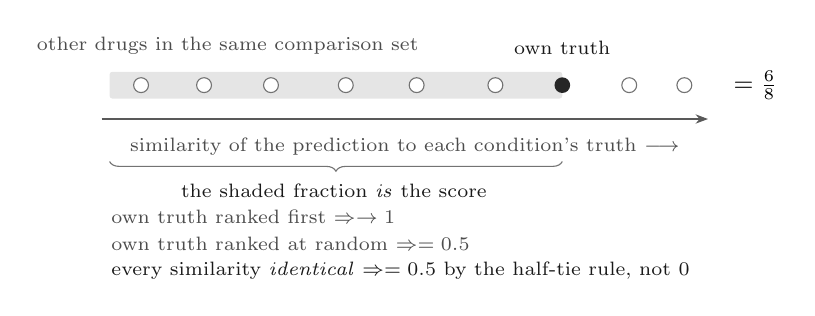
\begin{tikzpicture}[
  x=1cm, y=1cm, font=\small,
  lbl/.style={font=\scriptsize, text=black!70},
  strong/.style={font=\scriptsize, text=black!90},
  own/.style={circle, fill=black!85, inner sep=2pt},
  other/.style={circle, draw=black!55, fill=white, inner sep=1.9pt},
  ar/.style={-{Stealth[length=4.5pt]}, black!65},
]

\node[lbl, anchor=south] at (2.05,0.44) {other drugs in the same comparison set};
\node[strong, anchor=south] at (6.30,0.44) {own truth};

\fill[black!10, rounded corners=1pt] (0.55,0.00) rectangle (6.30,0.34);
\foreach \x in {0.95, 1.75, 2.60, 3.55, 4.45, 5.45} {\node[other] at (\x,0.17) {};}
\node[own] at (6.30,0.17) {};
\node[other] at (7.15,0.17) {};
\node[other] at (7.85,0.17) {};
\node[anchor=west, font=\small] at (8.35,0.17) {$\NIR = \tfrac{6}{8}$};

\draw[ar] (0.45,-0.26) -- (8.15,-0.26);
\node[lbl, anchor=north] at (4.30,-0.38)
  {similarity of the prediction to each condition's truth $\longrightarrow$};

\draw[decorate, decoration={brace, mirror, amplitude=3.5pt}, black!55]
  (0.55,-0.80) -- (6.30,-0.80);
\node[strong, anchor=north] at (3.40,-0.96) {the shaded fraction \emph{is} the score};

\node[lbl, anchor=west] at (0.45,-1.50) {own truth ranked first $\Rightarrow \NIR \to 1$};
\node[lbl, anchor=west] at (0.45,-1.84) {own truth ranked at random $\Rightarrow \NIR = 0.5$};
\node[strong, anchor=west] at (0.45,-2.18)
  {every similarity \emph{identical} $\Rightarrow \NIR = 0.5$ by the half-tie rule, not $0$};

\end{tikzpicture}
\caption[NIR is a discrimination score]{\textbf{$\NIR$ asks whether a prediction resembles its own
condition's truth more than it resembles the truths of the other conditions in the comparison set
$J$.} Own truth ranked first gives $\NIR \to 1$; ranked at random gives $0.5$; and a predictor whose
similarities are all identical --- the zero vector, which is what ``predict the average drug
response'' becomes in residual space --- scores $0.5$ by the half-tie rule, not $0$.}
\label{fig:nir}
\end{figure}


Our instruments compute $\NIR$ under three similarity functions and store all three:
\texttt{nir\_expr}, Euclidean distance in expression space; \texttt{nir\_rank}, the same
construction over rank vectors; and, in the residual frame of \S\ref{sec:methods-residual}, cosine
similarity between signed rank-discounted residual vectors. Every \emph{expression-frame} $\NIR$
figure in this chapter is \texttt{nir\_expr}. That choice is load-bearing, and it was not made by
the $\DRF$ audit below: \texttt{nir\_rank} never entered the graded family. It is excluded by a
cheaper admissibility screen that makes grading it pointless --- a held-out disjoint sample of a
condition's own cells must be retrievable above chance. Under \texttt{nir\_rank}, on the same
within-plate tier-2 run that later delivers the drug-blindness verdict ($n = 606$,
\texttt{nir\_sameplate.json}), every arm sits below the $0.50$ chance line and the noise ceiling is
among them: ceiling $0.380$, control-copy $0.337$, model $0.313$, drug-agnostic linear map $0.285$,
mean baseline $0.070$. A metric on which a disjoint sample of a condition's own cells cannot be
retrieved above chance is not measuring what its name suggests, and no $\DRF$ was needed to see it.
Nor does the exclusion contradict the calibration literature's preference for rank-based metrics:
the rank in $\NIR$'s construction is a ranking of \emph{conditions} by similarity, not of genes, and
the similarity itself is computed in expression space. That screen is an admissibility test rather
than a grade: it asks only whether a condition's own cells can be retrieved above chance, and leaves
to the $\DRF$ audit below how much of the range between a drug-agnostic baseline and a noise ceiling
the surviving variant spans. All three variants are stored; the graded one is named here so the artifacts cannot be
misread.

Choosing $\NIR$ over its rivals is itself a measurement, made with the framework of Miller
et al.~\cite{miller}, which grades each metric rather than each model by asking how well it
separates a positive from a negative control. The Dynamic Range Fraction is
\begin{equation}
 \DRF(m) \;=\; \frac{m(\textrm{pos}) - m(\textrm{neg})}{m(\textrm{perfect}) - m(\textrm{neg})},
\end{equation}
on a scale where $0$ is the drug-agnostic baseline and $1$ a perfect predictor. Here
$\textrm{pos}$ is an interpolated-duplicate noise ceiling --- a technical duplicate interpolated
toward the mean baseline with per-gene weights given by differential-expression significance ---
and $\textrm{neg}$ is a drug-agnostic leave-one-out mean. A negative $\DRF$ means the metric scored
the uninformative baseline above the noise ceiling in that run. Reading it as \emph{inversion} ---
the metric rewarding the generic gene ordering rather than the drug --- takes one further step,
that the sign is a property of the metric and not of the sample it was measured on. Three of the
four negatives below survive that step; the fourth does not, and is carved out where it appears. Three hardening choices matter for how the result can be read. Tied
expression values receive average ranks, because breaking ties by array index makes a tied gene's
rank depend on its position in the panel. The $\DRF$ ratio is recomputed whole inside every
bootstrap resample, because its denominator is estimated from the same data as its numerator and
holding it fixed understates the interval. And the family of five metrics is controlled
simultaneously with Holm's procedure, because the claim ``$\NIR$ alone points forward'' is a claim
about all five at once. Those three choices govern how the point estimate is formed. A fourth ---
what the bootstrap resamples --- governs whether the interval around it means anything, and in the
stored runs it was not made: each of the all-plates run's $1{,}820$ rows is one drug within one
cell line, and the resampler treated every row as its own cell line, against the $25$ that exist
(the same-plate run carried the identical defect over its own rows). The one-sided $p$ was read
off the observed resampling distribution rather than one with the null imposed, so it degenerates
to the floor $1/2001$ wherever $\DRF > 0$ and to $1$ wherever $\DRF < 0$, and no metric in the
family was in fact tested. Both are repaired in the analysis code and both arms have been rerun
under the repair. The same-plate rerun also fixed a mismatch the first run exposed: its cluster was
the (cell line, plate) pair the comparison is grouped within, but plates nest inside cell lines and
share their biology, so resampling pairs independently repeats the original error one level up. The
cluster is now the cell line in both arms, and the grouping unit and the cluster unit are reported
separately because they are not the same thing.

Under the hardened protocol, $\NIR$ is the only one of the five whose $\DRF$ is positive. In the
all-plates run, $\DRF(\NIR) = +0.635$, $95\%$ CI $[+0.604, +0.663]$, clustered on the $25$ cell
lines that the $1{,}820$ drug rows are nested in rather than on the rows themselves. The four rivals
are all negative and all exclude zero on the same clustering: $-0.163$ (\texttt{weighted\_r2}),
$-0.319$ ($\paneltau$), $-0.650$ (\texttt{spearman\_expr}) and $-0.686$ ($\DEdr$). Against a null
imposed by centring the resampling distribution at $\DRF = 0$, no draw of $2{,}000$ reaches the
observed value for $\NIR$, so the one-sided $p$ is at the resampling floor and reads $0.002$ after
Holm correction across the five metrics. That the $p$ is at the floor is now a statement about the
effect rather than about the resampler: the point estimate sits some forty cluster-robust standard
errors from zero. Restricting swap partners to the same plate ($586$ rows over $44$
cell-line$\times$plate groups spanning $27$ cell lines) pulls every value toward zero and changes no
sign: $\NIR$ $+0.545$ $[+0.516, +0.569]$, Holm $p = 0.002$ at the same resampling floor, against
$-0.104$, $-0.251$, $-0.500$ and $-0.515$ in the same order, each excluding zero. The two arms are matched on the thing the comparison is about ---
$27$ cell lines within plate against $25$ across plates --- which an earlier configuration was not:
capping the run at $25$ \emph{groups} admitted only $18$ distinct cell lines. That narrower run gives
$\NIR$ $+0.519$ $[+0.479, +0.546]$ over $335$ rows, so the figure is not an artifact of how many
plate-groups are admitted. What the argument uses is the sign pattern, which is identical in every
run for $\NIR$ and for the three rivals that carry a directional claim; no ranking among the
negative metrics is claimed. The inversion is a
property of the data, not a leak: a leave-one-out correction barely moves the numbers, since real
cell lines carry 20--204 drugs, and it survives holding the plate constant.

This replicates the methodological core of Miller et al.\ and then sharpens it. Metric choice
dominates, and the control-referenced correlation they flag is the worst performer in both arms
($\DEdr$, $-0.686$ across plates and $-0.515$ within). But their calibrated set does not transfer
intact to drug perturbation. The disagreement is specific: \texttt{weighted\_r2}, the counterpart
of the weighted $R^2\Delta$~\cite{mejia} that Miller et al.\ endorse, is negative in both audited
arms, though it sits closest to zero and its sign tracks cell count, so it carries no directional
claim of its own. Their endorsed rank-based $\NIR$ does survive. The inversions of $\paneltau$ over
the gene panel and \texttt{spearman\_expr} are separate rank-based failures: neither belongs to
Miller et al.'s calibrated set, so they are not evidence that the endorsed rank-based family was
ported and failed. What distinguishes $\NIR$ here is its \emph{discrimination} construction: it is
the only one of the five that scores a prediction against a set of other conditions rather than
against its own truth. Being rank-based alone is not what protects it; refusing to score anything
the generic response can supply is.
That is the statement worth carrying elsewhere, and it is not the one a clean replication would
have produced.

Miller et al.\ then conclude that under calibrated metrics deep models outperform uninformative
baselines; \S\ref{sec:res-blind} evaluates on the calibrated metric and finds the model at chance.
Two differences in setting are candidates for the discrepancy --- genetic versus drug perturbation,
and a discriminative regression model versus an autoregressive generative one --- and
\S\ref{sec:res-lookup} supplies a third and more structural possibility. Adopting their framework
is also deliberate in a second sense: evaluating our model on the metric their analysis endorses
means the drug-blindness result cannot be dismissed on the grounds their own paper raises.

\begin{figure}[htbp]
\centering
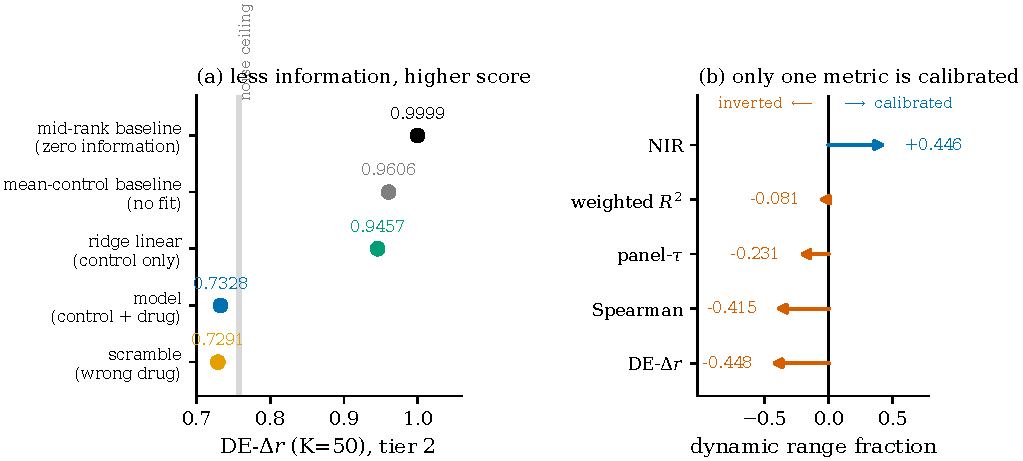
\includegraphics[width=\textwidth]{fig-calibration}
\caption[The standard metric is exploitable]{\textbf{Under the standard metric, less information
yields a higher score.} (a) A predictor carrying nothing about drug, cell or biology scores
$\DEdr = 0.9999$, above the two-real-cell noise ceiling and above the model. Tier 2, $n=400$
conditions. (b) Grading the metrics rather than the models: only $\NIR$ points forward. The panel
shows the same-plate run ($586$ rows over $44$ cell-line$\times$plate groups), the confound-free
version, in which $\NIR$ reads $+0.545$ against $-0.104$ (\texttt{weighted\_r2}), $-0.251$
($\paneltau$), $-0.500$ (\texttt{spearman\_expr}) and $-0.515$ ($\DEdr$); the all-plates run
($1{,}820$ rows over $25$ cell lines, one row per drug per line) gives $+0.635$ for $\NIR$,
$95\%$ CI $[+0.604, +0.663]$
clustered on cell line, with the four rivals between $-0.163$ and $-0.686$ and all excluding zero.
Both arms are clustered on the cell line --- $25$ across plates, $27$ within --- and every interval
shown is a percentile cluster bootstrap with no small-sample correction (see text). \texttt{weighted\_r2} carries no directional claim: its sign tracks cell count.}
\label{fig:calibration}
\end{figure}

Everything above grades \texttt{nir\_expr} only. The residual chapter scores a different $\sigma$
over a different comparison set, and a metric is not calibrated by having a relative calibrated, so
the residual frame carries its own $\DRF$ --- a second calibration result, on a different frame and
against different controls, rather than a formality discharged in passing. Computed on the same definition,
with a split-half replicate of the condition as the positive control and the drug-agnostic arms
already in the evaluation as the negatives, it reads $\DRF = +0.704$ $[+0.667, +0.736]$ against
\texttt{control\_copy}, clustered on the $42$ cell lines. It does not depend on which negative is
chosen: a random vector and the geometry-defined \texttt{orth} scrambled partner both give $+0.707$, and all three
negatives sit at chance as a matter of measurement ($0.506$, $0.501$, $0.501$) rather than of
stipulation. It is also reached under the more conservative of the two positive controls --- a raw
split-half replicate rather than the denoised interpolated duplicate the expression-frame protocol
uses --- so the residual frame is the better separated of the two ($+0.704$ against $+0.635$)
despite being graded against the harder reference, which is the direction the re-encoding was
intended to move. One arm is reported for completeness and carries no weight: \texttt{generic}
scores exactly $0.500$ with zero variance because the residual is defined by subtracting it, so
using it as the negative would make $\DRF$ a rescaling of the ceiling and test nothing.

One exception to the rule of \S\ref{sec:methods-data} is worth flagging where the numbers are, not
in a footnote. $\DRF$ is a ratio of means rather than a mean, and the two-way estimator above is
written for a mean, so both $\DRF$ intervals --- expression frame and residual frame --- are
\emph{one-way} percentile cluster bootstraps that resample whole cell lines and recompute the ratio
inside each draw. That respects the cell-line dependence and the ratio structure, and it ignores the
crossed well dimension. Wells are crossed with lines here, so the interval is robust on the
cell-line axis alone and is narrower than a fully crossed one would be. The $\NIR$ separation it
grades is far too large for that to change the sign, but the caveat belongs beside the number.

Two questions about the instrument remain, and they are not the same question. The first is whether
the conditions are empirically discriminable at the tested pseudobulk and cell budget: if a
disjoint sample of a condition's own cells cannot be told from another drug's cells there, no repair
to the metric would help on that instrument. A spike-in forced choice answers that narrower
question. Within one plate, a reference pseudobulk drawn from drug A's
cells must be scored more similar to a disjoint sample of A's own cells than to a sample of drug
B's, over many resamples, with chance at $0.50$; contaminating B's population with a growing
fraction of A's cells titrates the difficulty, so the curve of accuracy against contamination
characterises each metric's sensitivity. At zero contamination three of the six metrics scored
separate the two populations essentially perfectly ($\paneltau = 1.000$, $\DEdr = 0.995$, top-$n$
$\tau = 0.987$, plate held constant), and at full contamination those same three return
$0.501$--$0.502$. The whole-profile similarity scores on the same instrument are much weaker even at zero contamination
--- cosine $0.740$, Spearman $0.680$, cosine on the shift $0.620$ --- which is worth registering,
because a whole-profile similarity is what $\NIR$ uses in the expression frame. Lack of empirical
discriminability is not the sole bottleneck at this tested budget: split-half
retrieval establishes discriminability, not predictability from untreated input, and how much of it
a given $\sigma$ recovers is a separate matter.

The second question --- whether $\NIR$ itself registers a true positive --- the spike-in does not
answer, since $\NIR$ was not among the metrics run on it. The evidence is the positive control
inside the $\DRF$ audit, on the same two runs that produce the figures above: under $\NIR$ the
interpolated duplicate scores $0.802$ against the drug-agnostic mean's $0.457$ across plates, and
$0.668$ against $0.272$ within plate. In the residual frame a split-half replicate reaches $0.854$
against negatives at $0.501$--$0.506$. None of these is the reference the drug-blindness verdict is
measured against, and it is worth saying which is: the same within-well split-half precision
reference recomputed on the tier-2 within-plate benchmark, where it sits above chance but not far
above it. That --- rather than $1.0$ --- is the bar \S\ref{sec:res-blind} states the model against,
and it is quoted there with the verdict.

\begin{claim}
The field's standard score is saturated by a predictor carrying no information ($\DEdr = 0.9999$).
Of the five candidates audited, $\NIR$ is the only one with a positive $\DRF$ ($+0.635$,
$[+0.604, +0.663]$ on a one-way cluster bootstrap over the $25$ cell lines --- the declared
exception to this chapter's two-way rule --- Holm $p = 0.002$; $+0.545$ $[+0.516, +0.569]$
over $27$ cell lines with same-plate partners, Holm $p = 0.002$), and the other four are negative
with intervals excluding zero in both audited arms. Three of them --- $\paneltau$,
\texttt{spearman\_expr} and $\DEdr$ --- are inverted rather than merely uninformative, each
ranking the drug-agnostic baseline above the noise ceiling; \texttt{weighted\_r2} sits closest to
zero and its sign tracks cell count, so no directional claim is made for it. Under $\NIR$ the positive control is retrieved
well clear of the negative ($0.802$ against $0.457$ across plates, $0.668$ against $0.272$ within),
so the instrument registers a true positive. Every drug-use claim in the rest of this chapter that
rests on a continuous prediction score is therefore made on the calibrated metric; $\DEdr$ appears
below only where two arms are compared with each other on the same scale, never as an absolute score
of the model's drug use. The remaining instruments --- forced-choice grading, output invariance, and
the logit-space activation tests of \S\ref{sec:res-mechanism} --- are deliberately on scales of their
own, each with a fixed chance value or a paired control.
\end{claim}

\subsection{The model is drug-blind}
\label{sec:methods-controls}
\label{sec:res-blind}

With a ruler that cannot be gamed in hand, the investigation can ask the question it exists to
answer: does the model use the drug at all? The answer is no, and it is stated before the
instruments because the instruments matter only as the objections they close. On the calibrated
metric, within plate on tier 2 ($n = 606$), the model scores $0.498$ against a within-well split-half
precision reference of $0.576$. It is matched by predictors that know nothing about the drug: a drug-agnostic linear map
scores $0.500$, a control-copy $0.504$, the global mean $0.180$. And on the identifiable stratum,
whose own within-well reference clears the pre-set $0.80$ bar, a zero-drug-information control-copy reaches $0.766$ against
the model's $0.768$.

Four instruments produce this verdict, and each exists because a specific objection would otherwise
be fatal. They are the benchmark itself (the model against drug-agnostic baselines on the
calibrated metric, within plate); the scramble ablation (the only manipulation that isolates drug
use); forced-choice grading (a truth-based check whose chance value is fixed); and output
invariance (a truth-free check that no scoring choice can confound). The benchmark is the verdict
above; the other three are built and reported below.

One measurement rule comes first, because the verdict depends on it. Drug and plate are partially
confounded by the atlas's design (\S\ref{sec:methods-data}), so discrimination grouped by cell line
alone lets the batch signature stand in for drug identity. Measured directly, by scoring tier-2
conditions with and without the plate held constant --- not one fixed set of conditions on both
sides, because holding the plate constant costs every condition that has no same-plate comparison
set, so the within-plate column is the subset of the cross-plate one that survives that requirement
($998$ of $1{,}163$), and both are wider than the $n = 606$ benchmark the verdict above is stated
on:

\begin{table}[htbp]
\centering
\begin{tabular}{lrr}
\toprule
Predictor (drug-agnostic) & cross-plate & within plate \\
\midrule
mean baseline & 0.399 & \textbf{0.161} \\
control-copy & 0.551 & 0.510 \\
\midrule
noise ceiling & 0.625 & 0.575 \\
fraction of drugs at chance & 43\% & 49\% \\
\bottomrule
\end{tabular}
\caption{Expression-frame $\NIR$. A drug-agnostic mean baseline more than doubles its score when the
plate is free to vary, which is what plate leakage looks like. The ceiling falls once the plate is
held constant because the batch signature was inflating it too. This is the leak audit, a wider
diagnostic run than the $n = 606$ tier-2 benchmark the verdict above is stated on ($n = 1{,}163$
cross-plate, $n = 998$ within plate), so its within-plate figures sit slightly off the ones quoted
there: control-copy $0.510$ against $0.504$, mean baseline $0.161$ against $0.180$, and the
within-well split-half precision reference $0.575$ against $0.576$.}
\label{tab:plateleak}
\end{table}

The mean baseline is the clearest demonstration: it contains no drug information whatsoever, and it
scores $0.399$ when the comparison set may span plates against $0.161$ when it may not. Every
discrimination instrument therefore gained a \texttt{--same\_plate\_only} mode and all discrimination
results in this chapter were re-run within plate, except where a departure from that rule is named
at the point of use --- as with the swap-distance sweep that answers the fourth objection below,
whose swap partners were not plate-restricted (Appendix~\ref{sec:app-sweep}), and the residual-frame
scores of \S\ref{sec:methods-residual}, whose comparison set is grouped by cell line and whose
justification is given there. Conclusions are unchanged; some magnitudes shrink.

The central manipulation is the \emph{scramble ablation}: the prompt is left byte-identical except
that the drug name and mechanism are replaced by another drug's, while the control cell and the
scoring truth are unchanged. Because both arms share the same control cell, control- and
batch-derived leakage cancels in the scramble gap $\gap = \NIR_{\textrm{model}} -
\NIR_{\textrm{scramble}}$. This is the only manipulation that isolates drug use, and the only difference in this chapter whose
leakage cancels by construction. It does not displace the drug-agnostic comparisons: the verdict
above and the stratum ladder below are comparisons of exactly that kind, and what licenses them is
not cancellation but the within-plate rule Table~\ref{tab:plateleak} establishes. Both are reported
wherever both exist.

Two constraints on the swap partner are required for a gap measured this way to mean what it says,
and both exist because the unconstrained pool fails in a specific way. The partner must be a
different drug: allowing the same drug at another dose or plate substitutes the drug for itself, an
unchanged output is then correct rather than blind, and the contamination concentrates in the most
similar stratum because a drug's own other doses are usually its nearest neighbours. And the partner
must be on the same plate: residuals retain plate structure, so a cross-plate partner differs from
the target in batch as well as in drug, and the gap absorbs both. A scramble that swaps in a drug
with a similar true response is also a weak test, and in this atlas that risk is structural rather
than incidental. In full-profile space the mechanism annotation is close to uninformative about
transcriptional response: in the characterisation behind Table~\ref{tab:scale}, two drugs sharing a
\texttt{moa-fine} annotation sit a mean distance $2.322$ apart against $2.377$ for two drugs that do
not --- $1{,}244$ same-mechanism against $17{,}563$ different-mechanism pairs, a ratio of $0.977$.
Same-mechanism drugs in Tahoe are just over two per cent closer to each other than arbitrary pairs
are. That is a fact about the data rather than about the scramble, and it recurs: it is why
conditioning on mechanism fails to move $\DEdr$ in the grouping ladder below, and it is why the
scramble's own preference for a partner of different mechanism cannot on its own be relied on to
deliver a different response --- ``different mechanism'' does not imply ``different response''.
(Mechanism does carry signal in the residual frame, \S\ref{sec:res-scope}; the ladder below takes up
why the two are not in conflict.) Two remedies are used. A swap-distance sweep --- two hundred (drug, swap) pairs over
twenty cell lines on tier 2, binned by quantile of the response distance $\lVert y_A - y_B \rVert$
between the real and swapped-in drug --- turns the single test into a curve of $\gap$ against that
distance. And a stratified scramble defines three partners per condition, chosen by residual cosine
within the cell line: \texttt{near} (most similar), \texttt{orth} ($\cos\approx0$) and
\texttt{opposite} (most anti-correlated). The strata make visible an assumption that a single
comparator hides: the gap has two parts --- how much naming the truth helps, and how much naming a
lie hurts --- and only the first is wanted. A usable null is therefore a stratum whose own score
sits at chance. \S\ref{sec:res-generalisation} shows this is true of exactly one of the three, and
not the one an evaluation would naturally default to.

% fig-scramble.tex -- the scramble ablation and why its difference is leak-immune.
% No data dependency.
% Layout note: the prompt boxes are ~2.2cm tall once the shaded spans are set, which is far more
% than a four-line block looks like it should need. Every band below them is placed against that
% measured height, not against an estimate.
\begin{figure}[htbp]
\centering
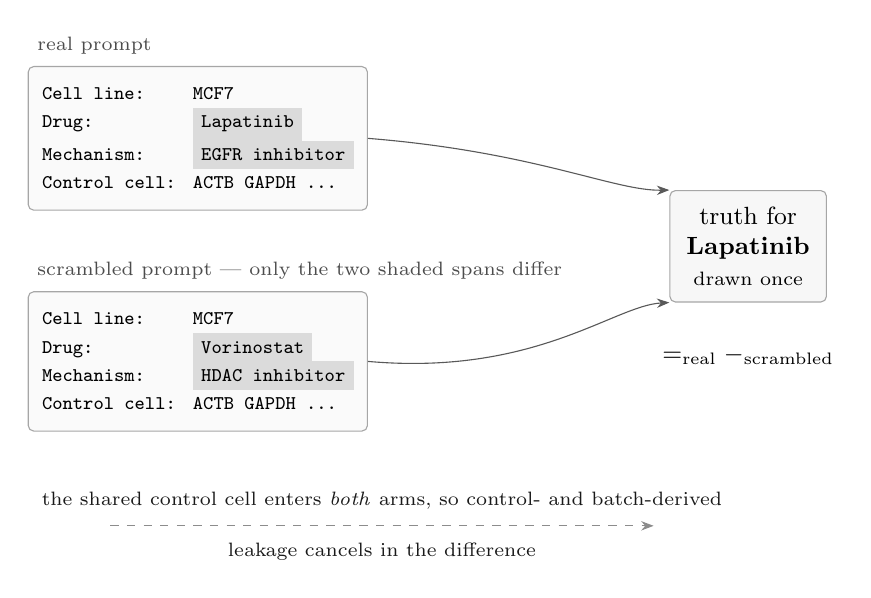
\begin{tikzpicture}[
  x=1cm, y=1cm, font=\small,
  lbl/.style={font=\scriptsize, text=black!70},
  strong/.style={font=\scriptsize, text=black!90},
  promptbox/.style={draw=black!35, rounded corners=2pt, inner sep=5pt, fill=black!2},
  ar/.style={-{Stealth[length=4.5pt]}, black!65},
]
\newcommand{\spanhl}[1]{\colorbox{black!14}{#1}}

\node[lbl, anchor=west] at (0.15,0.00) {real prompt};
\node[promptbox, anchor=north west] (p1) at (0.15,-0.26) {%
  \renewcommand{\arraystretch}{0.9}%
  \begin{tabular}{@{}l@{~~}l@{}}
  \ttfamily\scriptsize Cell line:    & \ttfamily\scriptsize MCF7 \\
  \ttfamily\scriptsize Drug:         & \ttfamily\scriptsize \spanhl{Lapatinib} \\
  \ttfamily\scriptsize Mechanism:    & \ttfamily\scriptsize \spanhl{EGFR inhibitor} \\
  \ttfamily\scriptsize Control cell: & \ttfamily\scriptsize ACTB GAPDH \ldots \\
  \end{tabular}};

\node[lbl, anchor=west] at (0.15,-2.86) {scrambled prompt --- only the two shaded spans differ};
\node[promptbox, anchor=north west] (p2) at (0.15,-3.12) {%
  \renewcommand{\arraystretch}{0.9}%
  \begin{tabular}{@{}l@{~~}l@{}}
  \ttfamily\scriptsize Cell line:    & \ttfamily\scriptsize MCF7 \\
  \ttfamily\scriptsize Drug:         & \ttfamily\scriptsize \spanhl{Vorinostat} \\
  \ttfamily\scriptsize Mechanism:    & \ttfamily\scriptsize \spanhl{HDAC inhibitor} \\
  \ttfamily\scriptsize Control cell: & \ttfamily\scriptsize ACTB GAPDH \ldots \\
  \end{tabular}};

\node[draw=black!35, rounded corners=2pt, inner sep=6pt, align=center, fill=black!3]
  (truth) at (9.30,-2.55) {truth for\\\textbf{Lapatinib}\\{\scriptsize drawn once}};

\draw[ar] (p1.east) .. controls (6.6,-1.35) and (7.6,-1.85) .. (truth.north west);
\draw[ar] (p2.east) .. controls (6.6,-4.20) and (7.6,-3.30) .. (truth.south west);

\node[anchor=north, font=\small] at (9.30,-3.70)
  {$\gap = \NIR_{\text{real}} - \NIR_{\text{scrambled}}$};

\draw[ar, dashed, black!45] (1.20,-6.10) -- (8.10,-6.10);
\node[strong, anchor=south, align=center] at (4.65,-6.02)
  {the shared control cell enters \emph{both} arms, so control- and batch-derived};
\node[strong, anchor=north, align=center] at (4.65,-6.20)
  {leakage cancels in the difference};

\end{tikzpicture}
\caption[The scramble ablation]{\textbf{The scramble replaces the drug name and its mechanism and
nothing else.} Both arms are conditioned on the same control cell and scored against the same truth,
so any leakage through the control cell or the plate enters both arms in equal measure and cancels in
the difference $\gap$. This is why $\gap$ is the only difference in the chapter whose leakage cancels
by construction, while a comparison against a drug-agnostic predictor is not leak-immune --- such a
baseline inherits whatever plate structure the comparison set carries
(Table~\ref{tab:plateleak}). Comparisons of that kind are used, and used centrally, with the
comparison set declared at every score: within plate in the expression frame, where the leakage is
controlled rather than cancelled, and by cell line in the residual frame, where the plate-scoped
generic has already subtracted each plate's mean response from truths and predictions alike --- in
expectation, with however much survives in an individual residual left unmeasured
(\S\ref{sec:methods-residual}, and \S\ref{sec:limitations} for what that leaves open).
A refinement matters here: if the swapped-in drug happens to have a
\emph{similar} true response then an unchanged output is correct rather than blind, so the swap
partner is chosen from three defined similarity strata by residual cosine. Which stratum can carry
the canonical magnitude associated with this figure is constrained by the comparator's own score.
\S\ref{sec:res-generalisation} finds the geometry-defined \texttt{orth} partner empirically near
chance at $0.501$ in this sample, making it the least contaminated available comparator rather than
an independently established null. That restriction belongs to this canonical scramble comparison:
the three-stratum repair comparison differences each model score against its own
\texttt{near}/\texttt{orth}/\texttt{opposite} partner, while field attribution uses its stated
span-specific partner and retains the resulting comparator caveat.}
\label{fig:scramble}
\end{figure}


The third instrument is forced-choice grading: a prediction is scored against its own condition's
truth and against another drug's truth from the same comparison set, recording how often the own
truth wins. Chance is $0.50$ by construction, and the precision reference --- the same forced choice
with a disjoint sample of the condition's own cells substituted for the prediction --- lands
between $0.67$ and $0.83$ depending on
cells per condition. The fourth is output invariance, which asks whether the drug token changes the
generated text at all, without reference to any truth. It is generated at $3800$ tokens, the
longest budget in the chapter, because it compares two generations to each other rather than to a
scoring panel and truncation would cut the comparison rather than the score. For a fixed control cell, the model generates
twice from the same prompt and once from each of several prompts differing only in the drug, and the
instrument compares
\begin{equation}
 \textrm{invariance gap} \;=\;
 \underbrace{\overline{\textrm{sim}}(\textrm{same prompt, resampled})}_{\textrm{sampling noise alone}}
 \;-\; \underbrace{\overline{\textrm{sim}}(\textrm{prompts differing in the drug})}_{\textrm{noise plus any drug effect}},
\end{equation}
with similarity measured as top-$100$ Kendall $\tau$ and as Jaccard overlap. A positive value means
two generations for the same drug resemble each other more than generations for different drugs do;
zero means swapping the drug perturbs the output no more than resampling at the same temperature
does. Reported over $8$ contexts $\times$ $12$ drugs at temperature $0.8$. This instrument is the
least informative of the four --- it can only detect whether the output moves, not whether it moves correctly
--- but it is also the least able to be confounded, since it needs no ground truth at all.

\begin{table}[htbp]
\centering
\footnotesize
\begin{tabularx}{\textwidth}{@{}>{\raggedright\arraybackslash}p{0.25\textwidth}
  >{\raggedright\arraybackslash}p{0.18\textwidth}
  >{\raggedright\arraybackslash}p{0.31\textwidth}>{\raggedright\arraybackslash}X@{}}
\toprule
Instrument & Quantity & Value & Reading \\
\midrule
Forced-choice grading & own-truth win rate & $0.48$ ($\approx$ scramble; ceiling 0.67--0.83) & chance \\
Output invariance & invariance gap & \ci{0.000}{-0.019}{+0.016} & bounded, $\leq 0.016$ \\
Scramble, tier 1 & $\DEdr$ & $0.740$ real vs $0.739$ scrambled & indistinguishable \\
Scramble, tier 2 & $\DEdr$ & $0.733$ real vs $0.729$ scrambled & indistinguishable \\
Scramble (identifiable subset) & $\gap$ ($\NIR$) & \ci{+0.014}{-0.016}{+0.042} & bounded, $\leq +0.042$ \\
\bottomrule
\end{tabularx}
\caption{Four independent instruments agree, and the two that return intervals bound the drug's
effect rather than merely covering zero; both bounds are read out below. Near-ceiling $\DEdr$ is
achieved identically with a wrong-mechanism drug, so that score is drug-independent.}
\label{tab:blind}
\end{table}

Two of the four return intervals, and an interval that covers zero earns its keep by what it
excludes, not by the word \emph{null}. The output-invariance gap is $0.000$
\nolinebreak[3]$[-0.019, +0.016]$ in top-$100$ Kendall $\tau$; two generations from a byte-identical
prompt agree at $\tau = 0.198$, so the interval caps any drug-driven divergence at roughly a twelfth
of the agreement two identical prompts retain, and the Jaccard version of the same comparison is
tighter still ($+0.000$ \nolinebreak[3]$[-0.008, +0.008]$). On the identifiable stratum the scramble
gap is $+0.014$ \nolinebreak[3]$[-0.016, +0.042]$, against the $0.170$ that separates the model's
$0.768$ from that stratum's $0.938$ ceiling: at the very top of the interval, naming the right drug
rather than a wrong one would buy a quarter of what is there to be bought, and the point estimate
puts it at $8\%$ of that. Neither figure shows the effect is zero and no experiment here could;
both put it far below the headroom these conditions leave. Read that way the result is
stronger than the word null, not weaker.

Four objections to the verdict close on measurement rather than argument. First, \emph{is there
anything to know?} A ladder of mean-shift baselines --- each predicting the average response of a
progressively narrower group --- answers that directly. On tier 2, predicting the global mean scores
$\DEdr$ $0.056$; conditioning on cell line raises it about two-and-a-half-fold to $0.142$;
conditioning on mechanism does not move it ($0.052$); and conditioning on mechanism and cell line is
no better than cell line alone ($0.120$ against $0.142$). Tiers 1 and 3 tell the same story. The
informative conditioning variable in this data is therefore the cellular context, not the compound
class. It is worth holding onto, because \S\ref{sec:res-used} finds precisely that asymmetry
inside the model's activations, and \S\ref{sec:res-scope} finds that mechanism does carry signal
once the generic programme is subtracted. The apparent tension is a frame difference rather than a
contradiction: in full-profile space the generic response dominates and swamps a mechanism effect
that becomes visible only in the residual frame.

Second, \emph{is the task empirically discriminable at the tested pseudobulk budget?} Only $46.2\%$
of (drug, cell line) conditions clear the identifiability bar of Table~\ref{tab:scale} --- their own
within-plate split-half $\NIR$ against their plate-mates reaching $0.8$ --- and $78.7\%$ have a
plate-mate closer to them than their own split-half replicate is. How inert the rest are depends on
what is asked. A whole-profile permutation test against DMSO
calls $72.7\%$ of the $5{,}014$ testable conditions active, leaving $27.3\%$ statistically inert; a
per-gene test is far harsher, and the median condition has no gene at all surviving BH correction at
$q < 0.05$ (Table~\ref{tab:scale}). The two do not contradict each other --- a whole-profile test
pools evidence that no single gene carries --- but $27.3\%$ quoted alone would make this atlas sound
better resolved than it is, and any gene-level reading of these conditions answers to the harsher
number.

Restricting to the identifiable subset does not rescue the model. It appears to beat the linear
baseline there ($0.768$ against $0.531$), yet a zero-drug-information control-copy reaches $0.766$
on the same conditions --- the paired model-minus-control contrast is \ci{+0.002}{-0.026}{+0.028}
--- and the leak-immune $\gap$ stays bounded as above. The model is drug-blind on the identifiable
stratum as well as overall.

The control arm carries a second result that is easy to walk past, and it constrains how a ceiling
of this kind should be read. Across the three strata the control-copy's score tracks the ceiling
almost step for step: $0.310$ against a ceiling of $0.287$ on the low-reference stratum, $0.540$
against $0.689$ on the marginal one, $0.766$ against $0.938$ on the empirically identifiable one. A predictor that reproduces
the untreated cell and knows nothing whatever about any drug does best exactly where the ranking
problem is easiest. The reading this invites is that what makes a condition identifiable on this
criterion is largely what makes its untreated cells distinctive among their plate-mates, rather than
what makes its drug's effect distinctive --- so the distance between a predictor and a high ceiling
is not all of it room that better drug modelling would fill. The ceiling itself rises with
aggregation ($0.61$ at 10 cells, $0.76$ at 40, $0.85$ at 120), so empirical discriminability rises
across these tested cell budgets; what the strata add is that most of the ranking it is scored on
can be done without the drug.

\begin{figure}[htbp]
\centering
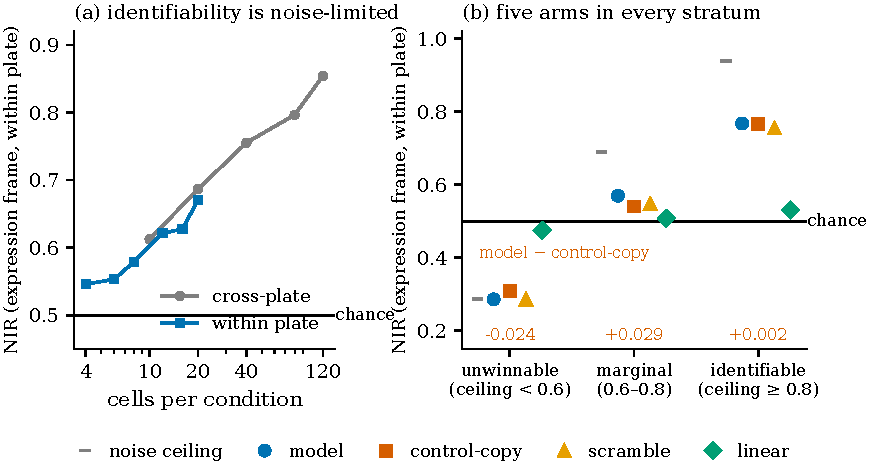
\includegraphics[width=\textwidth]{fig-difficulty}
\caption[Difficulty structure and the stratum ladder]{\textbf{Conditions are more empirically
discriminable at the tested pseudobulk budget where the noise ceiling is high, and precisely there,
a predictor containing no drug information matches the model.} (a) The ceiling rises steadily with the number of cells per condition, cross-plate and
within plate, so empirical discriminability rises with aggregation across the tested cell budgets.
(b) Conditions binned by their own ceiling, with five arms in every
stratum. On the identifiable stratum ($n=204$) the model reaches $0.768$ --- and a control-copy
baseline that simply reproduces the untreated cell, and therefore knows nothing whatever about the
drug, reaches $0.766$. The paired contrast beneath each stratum is
\ci{+0.002}{-0.026}{+0.028} there, clustered over cell lines. Showing the model alone across these
strata would make the visual claim that it does better on higher-reference drugs; the control arm is what
shows that it does not.}
\label{fig:difficulty}
\end{figure}

Third, \emph{does the representation throw the drug away?} Cell sentences keep only the rank order
of genes and discard expression magnitude, and if the drug lived in the magnitudes the diagnosis of
the following sections would be attacking the wrong thing. The objection is testable without any
model, by asking whether true expression discriminates drugs any better than rank does. It does not:
at single-cell resolution, cosine, Pearson and Spearman similarities on true normalised expression
all sit within $0.04$ of chance ($0.529$--$0.531$ [$0.515$, $0.543$]), the same near-chance regime
as rank. What recovers the signal is aggregation, not representation: at fifteen cells the
control-referenced shift cosine reaches $0.793$ [$0.775$, $0.809$]. The drug is not hiding in the
magnitudes, which matters twice over. It rules out the simplest alternative explanation for
everything that follows, and it means the repair of \S\ref{sec:res-encoding} cannot be read as
``restoring the magnitudes'': that repair keeps rank throughout and changes only what is being
ranked. The same measurement bounds the task from below --- at single-cell resolution the same-drug
versus different-drug discrimination gap is only $+0.006$ \nolinebreak[3]$[+0.003, +0.008]$, so
these instruments do not resolve drug identity from one observed cell at the available sequencing
depth and $946$-gene panel.

Fourth, \emph{does the scramble swap in similar drugs?} The swap-distance sweep bounds this rather
than settling it, and it sits outside the within-plate rule stated above: an earlier run with
\texttt{max\_new\_tokens=1200}
on the single-cell and optimal-transport checkpoints, scored on the unseen-drug tier of a different
evaluation set, with swap partners not restricted to the same plate, and with $n=40$ per bin wide
enough to exclude a large effect rather than to establish a null
(Appendix~\ref{sec:app-sweep}). Within that run neither column has an interval excluding zero in any
distance bin; in the single-cell column the far tail reads $-0.019$ across a $2.3\times$ spread in
swap distance, with a trend correlation of $+0.051$. That column therefore bounds a large
dissimilarity effect for the expression-frame model. The optimal-transport column cannot carry the
same bound: \S\ref{sec:res-encoding} later shows that checkpoint clears zero under the canonical
within-plate stratified test at the matched \texttt{max\_new\_tokens=1400} budget. Its apparent
null is therefore budget-dependent rather than a clean third leg of the drug-blindness result. The
stratified scramble replaced the sweep in the
reported set and is what carries the objection there.

\begin{claim}
On the calibrated metric the model is drug-blind in the expression frame, including on the
identifiable stratum: at chance overall ($0.498$ against a $0.576$ within-well split-half
precision reference), matched on the identifiable stratum by a
zero-drug-information control-copy ($0.768$ against $0.766$, paired contrast
\ci{+0.002}{-0.026}{+0.028}), and
no more moved by a maximally dissimilar swap than by a similar one in the single-cell column of a
non-canonical \texttt{max\_new\_tokens=1200} sweep outside the within-plate rule
(Appendix~\ref{sec:app-sweep}). The sweep's optimal-transport column does not carry that bound:
\S\ref{sec:res-encoding} later shows the same checkpoint is non-null under the canonical test at the
matched $1400$-token budget.
\end{claim}

\subsection{Is the drug represented at all?}
\label{sec:methods-probe}

A null result invites two readings, and they call for opposite repairs. Either the drug never
enters the model's computation --- an activation-side encoding failure, meaning that identity is not
written into the activations, which target- and input-side fixes might reach --- or it enters and is
ignored, a readout failure, which only an objective-side fix could reach. Every behavioural
measurement so far is consistent with both, because both predict the same
output. The previous section has already shown that the task is empirically discriminable for a
substantial stratum at the tested pseudobulk budget: the ceiling rises with aggregation, $46.2\%$ of
conditions clear the declared identifiability bar, and on those the model is matched exactly by a
baseline that copies the untreated cell ($0.768$ against $0.766$). So the shortfall on that stratum
is the model's, and the useful question becomes
where in the model it lives. That question cannot be answered behaviourally; it needs the weights.
It decomposes into three sub-questions, each with its own instrument, because each instrument's
blind spot is exactly what the next must close. Is drug identity present in the activations? Does
the network use the region where it is written? And when it uses that region, does it use which drug
is written there, or only that something is? This section answers the first; the next two take the
others in turn.

The first instrument is a linear decode probe, and its logic is deliberately weak in a way that has
to be said out loud, because the obvious reading of a probe result is the wrong one here. The prompt
names the drug in plain text (\S\ref{sec:methods-data}), so the drug is in the input by
construction, and a reader that recovers it from the activations has established only that the model
did not discard what it was handed. A positive was close to guaranteed. The informative outcome
would have been a negative --- the drug field already gone --- and what the probe buys, read as that
kind of floor test, is the depth at which such a negative would appear. No claim is made yet about
whether anything downstream reads what it finds.

The construction uses forward passes only, no generation and no training of the model itself. Real tier-2 evaluation
prompts are grouped by drug; for each, the residual-stream activation is captured at the last prompt
position, the position from which response generation begins, at every layer. A
cross-validated multinomial logistic-regression classifier then learns to name which of the twelve
drugs the prompt named, and its accuracy is compared against the floor measured on shuffled labels
($1/12 \approx 8\%$). The twelve drugs are a random draw from the tier-2 drugs with at least forty
scored cells each; the count sets the $8\%$ floor and, in \S\ref{sec:res-used}, bounds the drug
subspace at rank $11$. One limitation is stated rather than repaired: the cross-validation folds are
stratified over prompts and not grouped by well, so well-mates can straddle a fold boundary. The
accuracy is therefore read as a presence test, not a generalisation estimate, and the argument below
rests on the dissociation between decodability and the functional weight of the same region rather
than on the absolute figure.

The negative never arrives. The probe reads $82\%$ at layer 9 and $76\%$ at layer 16, the deepest
measured, against the $\approx 8\%$ floor; the between-drug to within-drug variance ratio collapses
about three-fold across the final layers, so the drug is present throughout but geometrically
de-emphasised as the output approaches. That de-emphasis belongs to the raw geometry, not to the
context-projected geometry used by the intervention that follows. Once cell line, plate and dose are
projected out, the corresponding context-projected probe series moves the other way, rising with
depth to $0.883$ ($88\%$) at the deepest layer. \S\ref{sec:res-used} defines that projection, reports
the full series and asks whether the network uses the region whose identity signal rises. The
dissociation is what motivates that instrument. The survival is what carries
weight here, not the peak: the
identity is still linearly available at the deepest layer measured, at the position the first
response token is emitted from, so nothing between the prompt and that layer has discarded it. That
is the end of what a probe can say. It is an external reader with access to information the
downstream layers may never consult, and whether the network itself reads this region is a causal
question --- the next section's.

\begin{claim}
The drug is not missing from the computation: its identity is linearly readable from the residual
stream at every layer measured. The raw probe reads $82\%$ at its layer-9 peak and $76\%$ at the
deepest against an $8\%$ chance floor; with cell line, plate and dose projected out the series rises
with depth instead, to $88\%$ at the deepest (\S\ref{sec:res-used}). The prompt names the drug, so
this is a floor test and its positive is close to free; what it
rules out is that the drug field is lost before the readout runs --- an encoding failure in the
activations --- and not that the readout ignores it. The drug is in the model; whether anything
inside the model reads it is the next question. (\S\ref{sec:methods-residual} later uses
\emph{target encoding} for a different thing --- how the target string is written --- and nothing
here bears on that.)
\end{claim}

\subsection{Is the drug-label activation signal used?}
\label{sec:res-used}

Asking whether the network uses the drug region means intervening on it, and intervening requires
localising it first. The second instrument is built in four steps, and each step exists because the
unguarded version of the same measurement misled us once already.

\emph{Step one: where the drug lives.} On $480$ tier-2 prompts --- twelve drugs, forty real cells
each --- at seven layers, the twelve per-drug mean activation vectors are centred on the global mean
and stacked, and their singular value decomposition contributes its top ten orthonormal directions:
$V_{\textrm{drug}}$, the slab of the residual stream in which drug identity is written. Twelve
centred class means span at most eleven directions, so the slab keeps essentially the whole span,
noisiest directions included; for a removal claim that choice is conservative. The layer grid is
even (2, 4, 6, 8, 12, 16) plus layer 9, added after the raw probe peaked there. A cell-line subspace
is built identically and serves throughout as the positive control, because the model demonstrably
does use cell line (\S\ref{sec:res-blind}'s grouping ladder).

\emph{Step two: purification.} The raw drug slab is partly a batch slab. Drugs are confounded with
plate and dose by the atlas's design, and probing dose from inside the drug subspace recovers it at
$0.90$--$0.95$ at every layer: read naively, the ``drug'' axis would partly be measuring the batch.
A context subspace is therefore built from the union of cell line, plate and dose directions, and
the drug axis is orthogonalised against all of it, giving $V_{\textrm{pure}}$ --- the part of the
drug axis not explained by batch. Every causal claim below is made on $V_{\textrm{pure}}$, never on
the raw slab.

\emph{Step three: the removal gate.} Before any ``ablating the drug changes nothing'' result can be
believed, the instrument must prove that the slab actually contains the drug. The decode probe's
accuracy is measured before and after projecting the drug subspace out, and the fraction of
above-chance signal removed must exceed $0.8$ --- otherwise the null is unfalsifiable, a measurement
of nothing. The gate passes at every layer: accuracy falls from $0.41$--$0.82$ to a constant $0.121$
floor, removing $88$--$95\%$ of the above-chance signal. The nulls below are real properties of the
model, not broken hooks.

\emph{Step four: the causal measurement, in logit space.} The true response is teacher-forced and
its per-token log-probabilities are read off clean; a forward hook then projects the slab out of the
residual stream at every position ($h \leftarrow h - (hV)V^{\top}$) and the log-probabilities are
read again; the measure is the mean KL divergence from clean to ablated over the response tokens, on
$60$ prompts. Scoring in logit space rather than by generating is a deliberate repair of the
project's first causal attempt, which injected a steering vector and generated: the steering vector
was small against the residual-stream norm, its effect on the output sat under the sampling-noise
floor, and its ``no effect'' was uninterpretable. The ablation is run for $V_{\textrm{pure}}$
(headline), for a random subspace of matched dimension (the null), and for the cell-line slab (the
positive control). The prompt count is small and no interval is quoted: the ablation is a
sign-and-magnitude instrument, and what intervals the probe arc has come from the identity test of
\S\ref{sec:res-mechanism} --- which is discounted there in turn, so no conclusion in this chapter
rests on the probe arc alone.

\begin{table}[htbp]
\centering
\begin{tabular}{lrrrrr}
\toprule
Layer & Decode & Decode & Ablate pure & Random & Ratio \\
 & (raw) & (context removed) & drug (KL) & matched dim & \\
\midrule
2 & 0.408 & 0.354 & 0.155 & 0.012 & $12.7\times$ \\
4 & 0.585 & 0.429 & 1.563 & 0.084 & $18.6\times$ \\
6 & 0.692 & 0.529 & 1.435 & 0.251 & $5.7\times$ \\
8 & 0.779 & 0.569 & 0.596 & 0.042 & $14.1\times$ \\
9 & \textbf{0.821} & 0.602 & 0.418 & 0.100 & $4.2\times$ \\
12 & 0.754 & 0.873 & 0.133 & 0.035 & $3.8\times$ \\
16 & 0.758 & \textbf{0.883} & 0.015 & 0.004 & $3.6\times$ \\
\bottomrule
\end{tabular}
\caption{All seven layers pass the removal gate (88--95\% of above-chance drug signal removed);
chance is $0.083$. The raw probe peaks at layer 9 and declines; with context removed, decodability
rises monotonically to layer 16.}
\label{tab:workspace}
\end{table}

\begin{figure}[htbp]
\centering
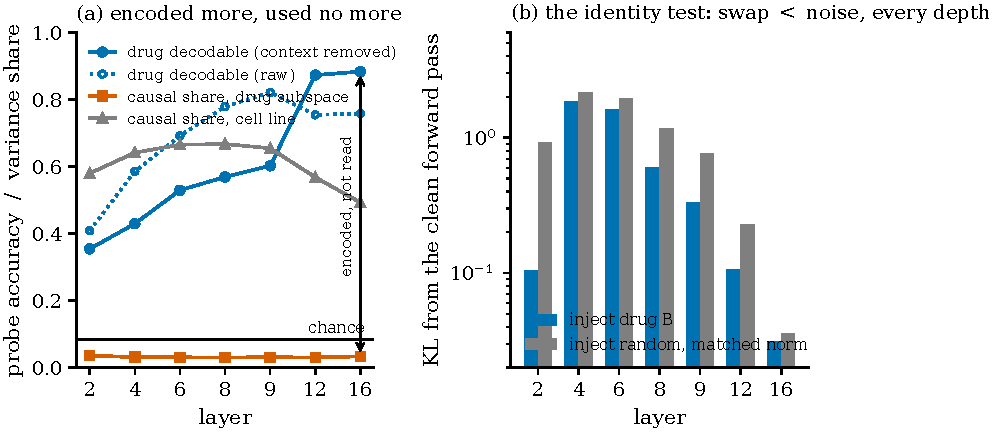
\includegraphics[width=\textwidth]{fig-mechanism}
\caption[Drug identity is increasingly decodable while its slab carries little functional weight]{\textbf{Drug-label information becomes more
decodable with depth while interventions on the purified slab have limited effect.} (a) Context-removed decodability by
layer, with the raw probe drawn for contrast. (b) Ablation of the purified drug subspace against a
matched-dimension random subspace, on a log axis because late-layer divergences are small for
everything. This is an intervention comparison; whether drug \emph{identity} is read requires
the substitution test reported in the text.}
\label{fig:mechanism}
\end{figure}

What the ablation shows is a dissociation, and Table~\ref{tab:workspace} quantifies it. With cell
line, plate and dose projected out, drug-label decodability rises with depth, from $0.354$ at layer 2 to
$0.883$ at layer 16: the supplied label becomes more linearly recoverable, not less. Yet the
purified drug-label slab's descriptive subspace fraction stays flat at $\approx 0.03$, against
$\approx 0.6$ for cell line --- an activation-space summary, not a decomposition of biological
drug-response variance --- and
ablating it costs $3.6$--$18.6\times$ the matched-dimension random null across layers. The ordering
is consistent across all seven layers under this sign-and-magnitude instrument. It is also small
beside the cell-line positive control, which the same ablation reads at
$1.0$--$11.2\times$ the drug's: removing the drug subspace costs $9$--$37\%$ of what removing cell
line costs at layers 2--9, with layer 12 the single exception at $98\%$ before layer 16 falls back
to $25\%$. On the descriptive subspace fraction the gap is wider still, cell line measuring
$15$--$22\times$ the purified drug slab. The intervention establishes sensitivity to removing an
activation-side drug-label signal, but at a bit player's weight under this instrument.

This is also where ablation reaches its limit as an instrument. It shows that the downstream
computation is sensitive to removing the slab; it cannot show that the slab's drug-specific
content is what is read: the purified directions could carry generic strong-programme energy that
merely co-varies with drug across twelve compounds. Whether the network reads which drug the slab
encodes requires replacing what the slab says rather than removing it, and that substitution test is
the next section's.

\begin{claim}
The purified drug-label slab carries decodable information and the output is sensitive to its
removal, but at a bit player's weight: once cell line, plate and dose are projected out, decodability
rises monotonically with depth --- the raw probe, which peaks at layer 9, does not --- while the
descriptive subspace fraction stays flat at $\approx 0.03$, roughly $5\%$ of the cell line's
$\approx 0.6$, and is not a biological variance decomposition; ablating the slab costs
$9$--$37\%$ of what ablating cell line costs at
layers $2$--$9$, with layer $12$ the single exception at $98\%$. Ablation cannot say whether the
slab's content is read --- that needs a substitution.
\end{claim}

\subsection{Is the drug's identity read?}
\label{sec:res-mechanism}

The verdict first, because the instrument that produced it runs for pages and the verdict is small.
In one of the five training arms of Table~\ref{tab:trainconfig}, at one depth of seven, injecting
half the class-mean displacement that points from drug A to drug B inside the purified drug subspace
($\alpha = 0.5$, the rung the multiplicity correction below is applied to) moves the model's
preference towards drug B's own held-out response --- relative to an identically constructed
injection that names a third drug --- by $+0.0197$ \nolinebreak[3]$[+0.0063, +0.0335]$ of the
preference gap the model already has. That is one to two
per cent, against a $10\%$ margin pre-registered for calling an effect material. Two further seeds
reproduce it, and of twenty-six headline tests it is the only survivor of multiplicity correction.
Read at face value that says the generation readout does consult which drug the region names, at a
gain far too small to account for anything in \S\ref{sec:res-blind}. Read with the multiplicity
discipline set out below it says less, because which result survives correction depends on which
rung of the magnitude ladder the correction is applied to and, at that rung, on which of the two
stored bootstrap draws is read. This is the weakest load-bearing
measurement in the chapter and it is carried as such: no argument downstream rests on it alone, and
a reader who discards it entirely loses nothing that the drug-blindness result depends on.

The instrument is nonetheless given at length, because an effect of one to two per cent is worth
reporting only if the design that produced it can be shown not to manufacture one --- and three
earlier versions of this design could not. The substitution test is the only instrument that can
answer the question at all, and the design that survived
audit is stated first; the three designs that failed are then the constraints it satisfies, one
sentence each, with their algebra deferred to Appendix~\ref{sec:app-identity}. The test makes two
structural choices so that its arms differ in nothing but which drug they name, and it ablates
nothing. First, a contrast score,
\begin{equation}
 \log P\!\left(g_B \mid \textrm{prompt}_A\right) \;-\; \log P\!\left(g_A \mid \textrm{prompt}_A\right),
\end{equation}
where $g_A$ and $g_B$ are real response strings emitted under drugs A and B by held-out cells, and
each log-probability is a per-token mean. Being a mean is what makes the contrast robust: any shift
that is uniform across positions --- an inflated logsumexp normaliser included --- enters both terms
equally and cancels exactly, whatever the two responses are and however many tokens each has. It
does \emph{not} cancel algebraically in the stronger sense one might assume. The normaliser is a
function of the hidden state, and once $g_A$ and $g_B$ diverge the two teacher-forced sequences
visit different states, so the state-dependent part of the normaliser differs between them and
survives the subtraction. That residual is not bounded here; what controls for it is the
\texttt{permuted} arm, which shares the anchor, the construction and the norm and differs only in
naming the wrong drug, so anything the contrast fails to cancel appears in that arm too. What
survives the comparison of the two arms is the model's preference between drug B's own held-out
response and drug A's. Second, every arm is anchored at drug A as an empirical class-mean
displacement of identical norm. Writing $\Pi$ for the orthogonal projector onto the purified slab, the
\texttt{swap} arm injects $\Pi(\mu_B - \mu_A)$, pointing at the drug whose response is scored; the
\texttt{permuted} arm injects $\Pi(\mu_C - \mu_A)$, rescaled to identical norm --- the headline
control: same anchor, same construction, wrong drug; and an isotropic random direction in the slab
is kept only as a damage diagnostic outside the empirical class-mean geometry, never as the
comparison, because a random direction can disrupt the model in ways an observed class-mean
displacement does not. The
subtraction $\mu_B - \mu_A$ cancels the global mean exactly, so the injected vector is a centred
between-drug class-mean difference within the purified slab; and no ablation anywhere means there
is no removed term for the control to trip over.

The three failed designs taught the constraints. A control drawn in the full $2048$-dimensional
stream puts $\approx 99.5\%$ of its energy where the intervention never acts, so the control must
live in the same subspace as the treatment. Ablate-then-add delivers (added $-$ removed), so an
uncentred class mean turns the substitution arm into a restoration --- hence no ablation, and an
exactly centred displacement. A norm-matched random direction falls outside the empirical
class-mean geometry and inflates the logsumexp normaliser (measured $+2.75$ nats), depressing every target whether or not it
carries identity --- which is what the contrast score and the \texttt{permuted} arm above are for.

What the planted-world selftest does and does not cover follows from the same algebra. It plants a
readout that genuinely reads the drug subspace and checks that the swap path recovers it, which
validates the directional logic end to end. It cannot speak to the normaliser, because in the
planted world each drug's ``response'' is a single token: there is no prefix, so nothing diverges,
and the one term the argument above had to be careful about is the one term the selftest never
exercises.

Everything is out of sample, and everything is on a comparable scale. The subspaces and class means
are fit on one slice of cells; $g_B$ is drawn from a third disjoint slice --- never from the rows
defining $\mu_B$, else the injected vector and the scored response would share cells and the test
would be partly circular; all scoring happens on the held-out slice. Because the five training arms
emit different target formats, raw log-probability differences live on different scales, so every
effect is divided by that model's own clean preference gap between A's and B's responses, measured
with no intervention: the reported unit is the fraction of the existing preference gap the injection
closes, comparable across arms.

Four guards carry the inference; the remainder --- a drug-proxy screen, an injected-norm diagnostic
and a three-world planted selftest --- are engineering and are deferred to
Appendix~\ref{sec:app-identity}. Uncertainty is a cluster bootstrap over ordered (A,B) pairs,
because rows sharing a pair share both the injected vector and the scored response; at the anchor
seed's layer $12$ that is $60$ rows in $58$ pair clusters over $24$ anchor drugs, so the resampling
sits close to a row bootstrap and guards against sharing within a pair but not against sharing
across pairs that share an anchor drug or a target drug --- rows naming the same target draw on
that drug's estimated class mean and on the same pool of held-out responses. Equivalence is by a criterion deliberately stricter
than TOST: the interval must lie inside a pre-registered margin, set at $10\%$ of the model's own
clean preference gap, \emph{and} contain zero. The second conjunct is not part of TOST and it runs
one way only --- it can withhold an equivalence verdict, never manufacture one. Under textbook TOST
the headline $+0.0197$ \nolinebreak[3]$[+0.0063, +0.0335]$ lies wholly inside the margin and would
be returned as equivalent, and read as a null; the rule used here returns a directional effect
smaller than the margin. A per-layer headroom gate excludes any layer
where the cell-line positive control shows less than $5\times$ dynamic range, because a saturated
instrument can support neither verdict. And a magnitude ladder repeats the test at $\alpha \in
\{0.5, 1, 2, 5, 10\}$ times the natural displacement, because a real identity effect should show a
monotone dose--response.

This design was run across the five training arms of Table~\ref{tab:trainconfig} and, for the two
residual arms, replicated at three further seeds. Of $26$ headline tests --- five arms by up to
seven depths --- exactly one survives Benjamini--Hochberg correction: the residual arm at layer $12$
($q = 0.026$, pooling the $26$ tests across the five arms rather than correcting within each arm as
the pipeline stores them). The $p$ behind that $q$ is a bootstrap quantity, and the residual arm's
own probe file carries
two draws of it for the same effect --- identical to sixteen digits --- at $p = 0.001$ and
$p = 0.004$, which fall either side of the $0.05/26$ the procedure admits at rank one; recomputed
across all $26$ on the second draw, nothing survives. The consensus arm at layer $2$ ($p = 0.012$)
does not survive ($q = 0.156$).

Which rung that correction is applied to matters, and the answer is not the one a reader would
assume. The headline is the $\alpha = 0.5$ rung --- half the natural displacement --- and the
ladder's first entry is therefore the headline restated in raw nats ($+0.0013$) rather than an
independent point beside it. At the full displacement $\alpha = 1$ the effect is \emph{larger} and
noisier: $+0.0265$ \nolinebreak[3]$[+0.0021, +0.0524]$ against $+0.0197$
\nolinebreak[3]$[+0.0063, +0.0335]$, at $p = 0.033$ against $p = 0.001$ on the draw the correction uses. Each of $\alpha = 0.5$, $1$
and $2$ excludes zero on its own and the two highest rungs do not ($\alpha = 5$ and $10$ span zero,
as an empirical class-mean displacement amplified far beyond its observed scale can). In raw nats
the five rungs read $+0.0013$, $+0.0017$, $+0.0044$, $+0.0061$, $+0.0046$: rising to $\alpha = 5$
and turning over at $\alpha = 10$. That is consistent with a dose--response and does not establish
one. All five rungs re-score the same $60$ rows at scaled injection rather than drawing
independently, no trend statistic is computed anywhere in the probe, and the monotonicity
pre-registered above holds over four rungs of five. But applying the $26$-test correction to the
$\alpha = 1$ slice instead
leaves \emph{nothing} surviving, and applying it to $\alpha = 2$ promotes a different arm at a
different depth (\texttt{residual\_holdout} at layer $4$, $q = 0.007$) while demoting this one. The
slice decides not merely whether a survivor exists but which one it is, and below that the
bootstrap draw decides whether one exists at all, which is the signature of a
family dominated by noise rather than one containing a single robust effect. The
multiplicity-corrected claim is therefore a statement about the $\alpha = 0.5$ slice and is not
robust to that choice --- which is why this section opened by discounting its own result rather
than closing on it.

\begin{table}[htbp]
\centering
\begin{tabular}{lrrr}
\toprule
Arm / seed & effect & 95\% CI & $p$ \\
\midrule
residual, seed 42 & $+0.0197$ & $[+0.0063, +0.0335]$ & $0.0010$ \\
residual, seed 43 & $+0.0118$ & $[+0.0060, +0.0173]$ & $0.00025$ \\
residual, seed 45 & $+0.0085$ & $[+0.0029, +0.0143]$ & $0.0015$ \\
\midrule
single-cell arm, six depths & \multicolumn{3}{l}{nothing detectable at any depth (median $-0.0012$)} \\
\bottomrule
\end{tabular}
\caption{The identity test, as a fraction of that model's own clean preference gap between the two
responses being compared (mean effect $+0.0133$ across the three seeds that measured it). The $p$
column is a two-sided cluster bootstrap over $4000$ resamples floored at $1/4000$; seed 43's entry
is that floor, reached when no resample fell at or below zero, so it is a resolution limit and not
a measurement. Seed 44
produced no layer-12 measurement: five of its seven layers were skipped because the purified slab
retained context, not for want of headroom --- the five carry headroom of $9.7$ to $23.3$, all well
clear of the gate. So the pre-registered criterion of two replications in three new seeds is met
with the third a non-measurement rather than a failure.}
\label{tab:identity}
\end{table}

The value of this is that it is a positive control on real data, and the argument for it borrows a
measurement this chapter does not report until several sections later. The residual arm is
independently known to respond to the drug its prompt names: on \texttt{train}, swapping the named
drug and its mechanism for an orthogonal partner costs it $+0.0898$ in $\NIR$, excluding zero
clustered on cell line ($[+0.0382, +0.1415]$) and on drug ($[+0.0291, +0.1506]$). That is a
behavioural result, measured without touching an activation, and it is established in
\S\ref{sec:res-generalisation}; used here it is a forward reference, and a reader unwilling to take
one on credit should read that section before accepting this control. Three things bound what it
licenses. It is a training-split fact --- the same establishment does not extend to held-out
combinations --- so the independent knowledge this control rests on is knowledge about that arm on
conditions it was trained on. It is behavioural, so it says the arm responds to the drug its prompt
names, not that the response is routed through the subspace this test injects into. And the two
measurements are not on the same weights: the swap gap is scored on the rebuilt target build and
this probe on the earlier one (Table~\ref{tab:trainconfig}), so drug-sensitivity and identity
reading are attributed here to residual-target training and not to any one checkpoint. What the
pairing buys is narrower than a routing claim, and it is enough: the probe detects identity reading,
replicably, in the arm behaviour calls drug-sensitive, and detects none at any depth it could
measure in the arm that is behaviourally drug-blind. A null from an instrument that has never been shown to register a
positive is uninterpretable; this one has.

\begin{claim}
The generation readout is sensitive to the drug-label activation signal at very low gain:
$+0.0197$
\nolinebreak[3]$[+0.0063, +0.0335]$ of the model's own preference gap in the anchor seed and
$+0.0133$ averaged over the three seeds that measured it --- one to two per cent, a fifth or less of
the $10\%$ margin pre-registered for calling an effect material --- in one training arm and at one
rung of the displacement ladder. The multiplicity-corrected version of that statement holds for the
$\alpha = 0.5$ rung on one of its two stored bootstrap draws, and not for its neighbours: at
$\alpha = 1$ nothing survives correction, and at
$\alpha = 2$ a different arm does. The claim is not that the readout cannot read drug
identity, and it is not the stronger mechanistic story that earlier drafts of this thesis told.
\end{claim}

Three limits belong with it. The effect appears at one depth of seven, and layer 4 is positive in a
single seed and null in the other three, which is what multiplicity discipline is for. The
single-cell arm has no layer-12 measurement at all --- its cell-line positive control reached
$3.88\times$ there, under the $5\times$ headroom gate, so the layer was excluded --- meaning the
cleanest comparison, the same depth across two arms, does not exist; the dissociation rests on that
arm being null at all six depths it could measure. And the sibling residual-holdout arm does not
reproduce the effect at the headline rung ($+0.0028$ and $+0.0049$ in the two seeds where it was
measured) --- it is instead the arm that surfaces at $\alpha = 2$, which is the rung-dependence
stated above rather than a second replication. Read together
with the decodability series, the picture is label information that becomes more linearly decodable with depth
once cell line, plate and dose are projected out --- the raw probe peaks at layer 9 and declines ---
while the process that writes the output barely consults it. That is suggestive of the workspace
account of Section~\ref{sec:lit-interp}, and it is offered as an interpretation of the pattern
rather than as a demonstration of the mechanism.

\subsection{Denoising the target: three nulls at one scoring}
\label{sec:res-epsilon}

That interpretation is not established, and this section does not proceed as though it were. What it
does is test the cheapest thing the interpretation predicts, which is worth testing on its own
account because it is the family of repairs a reader reaches for first. The prediction: if the
defect is a readout that barely consults the direction of the drug region, whatever is written
there, then improving what sits in that region cannot help --- and improving the training target is
exactly that kind of intervention. The inference runs one way only. A positive here would tell
against the low-gain reading; a negative is evidence about target-side fixes and not confirmation of
the mechanism. The obvious objection is that one failed target construction proves
nothing, so two further constructions were compared with it. The three points are the original
single-cell target, one optimal-transport barycentre and the consensus target.
\emph{Consensus} groups cells by (drug, cell line, dose) and averages them into one pseudobulk
sentence, with every original prompt retained so only the response changes. \emph{Optimal transport}
uses the full condition key carried by the source --- (cell line, plate, drug, dose/treatment well)
--- and computes each condition separately. Its treated cells are coupled only to the shared DMSO
controls from that condition's own (cell line, plate); treatment conditions are never pooled into
one coupling. The condition-specific coupling $\pi$ minimises
$\sum_{ij}\pi_{ij}\lVert x_i - y_j\rVert^2$ under balanced uniform marginals. Those marginals impose
mass conservation between the empirical control and treated measures; that balance is a modelling
assumption, not an observed biological constraint. Sinkhorn
iteration~\cite{cuturi} solves the coupling on the kernel $\Gamma = \exp(-C/\varepsilon)$, with $C$
the pairwise squared-distance matrix; couplings are computed in the released Tahoe scVI
latent~\cite{scvi} ($n_{\textrm{latent}} = 10$), joined per cell by barcode rather than re-encoded ---
a re-encode produced a degraded latent (cell-line probe $0.11$ versus $0.975$ for the shipped latent)
--- and targets are built decoder-free as convex combinations of that condition's observed treated
cells in expression space, so they remain inside their convex hull, not necessarily on the data
manifold. The regularisation
parameter locates the middle construction between two limiting cases:
$\varepsilon\rightarrow\infty$ gives a uniform
coupling and hence the treated mean (consensus); $\varepsilon\rightarrow 0$ gives a coupling
approaching an unregularised sparse transport solution, not necessarily a map to one
observed treated cell. Only three hand-picked constructions were trained and scored, so this is a
three-point comparison rather than a sweep of the regularisation family. It is a comparison at one
generation budget and against one comparator, and the caption records the point that a differently
scored evaluation does not find null. Every point was scored on the identifiable stratum --- the conditions
\S\ref{sec:res-blind} selected because their own within-well reference clears the pre-set $0.80$ bar
--- under the random-partner scramble
defined there.

\begin{table}[htbp]
\centering
\begin{tabular}{llrl}
\toprule
Target & $\varepsilon$ & $\gap$ & Verdict \\
\midrule
single cell (real treated cell) & $\approx 0$ & \ci{+0.014}{-0.016}{+0.042} & not separated \\
OT barycentric & $0.5$ & \ci{-0.001}{-0.018}{+0.016} & not separated \\
consensus (global mean) & $\rightarrow\infty$ & \ci{-0.010}{-0.022}{+0.003} & not separated \\
\bottomrule
\end{tabular}
\caption{The three target constructions form a three-point comparison, and no point separates from
its random-partner scramble on the identifiable stratum
($n = 204$). Two things bound how far that negative reaches. The consensus endpoint is the comparison's
weakest-evidenced point --- that arm was stopped at roughly $60\%$ of an epoch and its tier-1 NIR
was unscoreable --- so within this table the negative is carried by the single-cell and
optimal-transport endpoints, and the optimal-transport endpoint is not null in every frame. These
rows score it on the identifiable stratum against a random partner at a $1200$-token generation
budget; a separate evaluation of the same checkpoint, scored against the geometry-defined
\texttt{orth} partner over all its conditions rather than this stratum, moves from $+0.0144$
\nolinebreak[3]$[-0.0051, +0.0338]$ at $600$ generation tokens ($n = 250$) to $+0.0292$
\nolinebreak[3]$[+0.0144, +0.0441]$ at the residual arm's $1400$ ($n = 248$), reported in
\S\ref{sec:res-encoding}. This table's $1200$ tokens are a third budget, lying between those two,
and \S\ref{sec:methods-data} shows the budget is a claim-level variable in this project rather than
a runtime setting --- so the two frames differ in comparator, population and budget at once. That
point has not been re-scored on this table's terms, so the two frames are set side by side and not
put into ratio. The table is a null under this scoring, not a null over the family of target
constructions: outside this scoring the single-cell point is the only one whose negative survives a
matched budget and the geometry-defined \texttt{orth} partner, whose observed score is near chance.}
\label{tab:epsilon}
\end{table}

Training was not inert, and what it did instead is a result rather than an aside. The consensus
model stops echoing the control: on the identifiable stratum it scores $0.653$ against a
zero-drug-information control-copy at $0.766$, where the single-cell model sits on the control at
$0.768$. Its predictions are not mode-collapsed either --- there is real between-condition
variation. But that variation is uncorrelated with real drug identity: the Mantel correlation
between the model's between-drug distance structure and the true one averages $+0.03$ over
cell-line and plate groups. The failure this literature names first for a perturbation model that
underperforms on well-calibrated metrics is mode collapse --- the prediction ignores the input and
reverts to a mean, and the repair is to restore output diversity~\cite{mejia}. This arm is not
that. It moved off the control, it kept the variation, and it spent it on the wrong axis. Producing
no structure and producing structure that does not track the drug are different failures with
different repairs, and diversity restoration addresses only the first.

\begin{claim}
No point in the three-point comparison separates from its scramble on the identifiable stratum under the
random-partner test. Two things bound that negative: the consensus arm was stopped mid-epoch, so
within the comparison it rests on the single-cell and optimal-transport points, and the
optimal-transport arm is not null in every frame --- scored against the geometry-defined
\texttt{orth} partner over all
its conditions at the residual arm's generation budget, its gap excludes zero
(\S\ref{sec:res-encoding}). By the inference rule stated above that positive tells against the
low-gain reading rather than for it; it is measured in a different frame and so does not settle the
matter, but it is one more reason the interpretation of \S\ref{sec:res-mechanism} is carried here as
an interpretation and not as a result. What the three-point comparison establishes is that denoising the target changes what is
in the target without changing what the readout does with it under this scoring --- not that no
target-side fix can work. The next two sections turn to a different property of
the target --- how much of it its tokens expose to the drug, and how much drug-specific signal it
carries. Measuring those is not the same as showing that the target encoding is the defect, for the
reason given where the residual target is defined (\S\ref{sec:methods-residual}): that construction
changes five things at once.
\end{claim}

\subsection{The residual frame: predicting only what makes this drug different}
\label{sec:methods-residual}

If the \emph{target} encoding is the constraint --- how the target string is written, a different
sense of the word from the activation-side encoding ruled out above --- the target must be redefined
so that its tokens are the drug-specific part. How little of the standard target the drug occupies is measurable directly, and
the measurement motivates everything that follows. Because a cell sentence ranks genes by
expression, the target strings for two drugs in the same context are nearly identical, and the loss
weights every token position equally. The measurement counts, for pairs of drugs sharing a context,
how many of the $200$ target positions carry a different gene in the two drugs' target strings,
averaged over pairs; the precision-reference column scores within-condition split-half drug retrieval
through each row's own representation. The two columns are different quantities --- a count out of
$200$ positions and a retrieval score --- so what compares is the rows within a column, not the
columns with each other.

\begin{table}[H]
\centering
\footnotesize
\begin{tabular}{lrr}
\toprule
Representation & Top-200 tokens differing between drugs & \shortstack[r]{Within-well split-half\\retrieval reference} \\
\midrule
full profile (the standard target) & \textbf{34.6 / 200 (17\%)} & 0.742 \\
shift (treated $-$ control) & 111.4 (56\%) & 0.742 \\
\textbf{residual (drug-specific)} & \textbf{118.2 / 200 (59\%)} & 0.7432 \\
\bottomrule
\end{tabular}
\caption{$83\%$ of the standard target's tokens are identical between any two drugs in the same
context. The residual row is quoted at cell-line scope; at plate scope it reads $120.3$ and
$0.7467$. The third column is a split-half retrieval reference, not a biological replicate ceiling:
it scores disjoint cell subsets of one drug in one cell line on one plate against each other. It is
near-constant across the three rows; what the target encodings differ in is the second column ---
how much drug-discriminating content lands in the top-$200$ token positions. That is a fact about the
target's tokens; it does not on its own identify tokenisation as the binding constraint.}
\label{tab:divergence}
\end{table}

A second, descriptive summary is computed at plate scope, the scope used to construct the trained
residual target (\path{target_divergence_strat.json}). Its aggregate residual divergence is $120.3$;
the $118.2$ printed in Table~\ref{tab:divergence} is the corresponding cell-line-scope value. The
plate-scope summary enumerates $212{,}528$ exhaustive within-group drug pairs and asks whether the
aggregate hides a dependence on response similarity. Every representation is binned on the
\emph{same} axis, the cosine between the two residual responses, using the same fixed near,
orthogonal and opposite cut points as the later evaluation. These exhaustive bins are not the
later per-condition extreme-partner draws. For near, orthogonal and opposite pairs respectively,
the mean number of differing top-$200$ genes is $32.5$, $34.6$ and $35.8$ for the full profile;
$107.4$, $111.3$ and $114.4$ for the treated-minus-control shift; and $118.4$, $121.0$ and $118.7$
for the residual. The corresponding Spearman coefficients between residual cosine and target
divergence are $-0.149$, $-0.282$ and $+0.019$. Thus residual-target differentiation remains high
across all three strata and lacks the monotone dissimilarity gradient present in the full and shift
targets. This weakens the explanation that the later swap-distance pattern is inherited trivially
from residual-target divergence; it is not an independent test of that model result. The pairs reuse
drugs and experimental groups, so this stratification is descriptive and no pair-level inferential
claim is made.

The natural inference is that only a small fraction of the gradient can be carrying drug identity.
That inference is a hypothesis about the optimisation: what is measured here is the overlap of the
target gene sets, not a token-level loss or gradient attribution, and it should be read at that
strength. Its warrant is predictive --- it explains why every change to target content failed
identically in \S\ref{sec:res-epsilon}, and it predicts that changing what the tokens encode would
not. That warrant does not identify tokenisation as the unique binding constraint. Gene positions
are not loss-token positions under byte-pair encoding, and the residual target defined below alters
aggregation, control referencing, generic subtraction, sign coding and sequence length at the same
time as it alters token divergence. Separating those factors needs a matched-budget factorial that
this thesis does not run.

The residual target is the repair. For each condition (drug, cell line, plate, dose) with at least
$40$ treated and $20$ plate-matched control cells:
\begin{equation}
 \resid(d,c) \;=\; \underbrace{\big(\bar{y}_{\textrm{treated}} - \bar{y}_{\textrm{control}}\big)}_{\shift(d,c)}
 \;-\; \underbrace{\frac{1}{|D_c|}\sum_{d' \in D_c} \shift(d',c)}_{\textrm{generic}(c)} .
\end{equation}
The control subtraction removes the cell's own state; the mean-over-drugs subtraction removes the
generic drug programme shared across compounds. What remains is not what makes this drug different
from all drugs: it is what makes it different \emph{from the other training drugs that happen to
share its plate and cell line}. The comparison set is fixed by the plating design rather than
chosen, so the same compound plated among different neighbours would carry a different residual and
a different target string. That is the price of estimating the generic locally.

The generic is a plate-local mean, so whatever a compound shares with its plate-mates leaves along
with the stress and cell-cycle programme. Mechanism is the one channel where that matters:
\S\ref{sec:res-scope} finds mechanism-related drugs co-plated $0.404$ of the time against $0.362$
for a random draw, the only channel where the difference is material. For a co-plated mechanism
class, then, part of the class's own shared programme sits inside the generic and is subtracted out
of every member's residual by construction --- so the mechanism channel is graded in a frame that
has already removed some of what it is asked to find, and the bias runs against it.

The direction is testable rather than arguable. Joining Tahoe's \texttt{moa-fine} labels to the
plate rosters the gate itself scored, same-mechanism plate-mates supply a mean $4.4\%$ of a
condition's generic, small per condition but present for $83\%$ of the $917$ labelled
mechanism-arm conditions. The $155$ conditions with \emph{no} same-mechanism plate-mate --- whose
residuals therefore retain the mechanism programme --- give a gap of
\ci{+0.1145}{+0.0276}{+0.2014}, against \ci{+0.0737}{+0.0150}{+0.1324} for the $762$ that have one,
both against the same plate-matched null under the same two-way clustering. That is the direction
the construction predicts. It is not a corrected estimate: the two intervals overlap across almost
their whole range, the split is post hoc, and the cleaner stratum rests on $43$ wells. What it
supports is a statement about sign rather than size --- the frame understates this channel rather
than flattering it, which makes \S\ref{sec:res-scope}'s inconclusive verdict on mechanism the
conservative reading rather than a generous one.

The two subtractions are not equal partners, and the table above says which does the work. Removing
the control moves the between-drug token difference from $34.6$ to $111.4$; removing the generic
adds a further $6.8$ at cell-line scope and $8.9$ at the plate scope this build uses, so $92\%$ of
the recoverable difference --- $90\%$ plate-scoped --- is bought by the control subtraction alone. Almost everything the standard target hides is hidden by the cell's own baseline. That is a
property of the target encoding rather than a bad choice of target on our part: a list ranked by
absolute expression puts the same highly expressed genes at the top whatever the compound, so what
distinguishes two treatments has to fit into the positions the baseline ordering leaves free. The
measurement behind that reading is an overlap of gene sets, not a variance decomposition, and it is
one atlas at $K = 200$ ($6{,}602$ conditions, \texttt{target\_divergence.json}); how much of that ordering
a perturbation displaces is an empirical quantity, so no margin is claimed for other atlases or
other $K$. It is also the correct reading of \S\ref{sec:res-metrics}: what saturates $\DEdr$
there is reversion toward a central point, with \texttt{revert\_center} scoring $0.9999$ without
fitting anything at all, rather than the generic drug programme specifically. The generic is
nonetheless a real and separable component --- it carries $39\%$ of the shift's energy
(\S\ref{sec:res-transfer}) --- and subtracting it is what isolates the drug-specific remainder once
the baseline is already gone, at the price established above: where a mechanism class is co-plated,
part of what the mechanism channel is later graded on leaves inside the generic. The inclusion thresholds are
set where the identifiability curve of \S\ref{sec:res-blind} flattens: the within-well split-half precision reference is
$0.61$ at $10$ cells, $0.76$ at $40$ and $0.85$ at $120$, so below $40$ treated cells a condition is
still paying steeply for cells it does not have. Four properties of how the generic is estimated
decide whether the remainder can be trusted, and each was forced by a measured failure.

First, the split precedes the fit. An earlier build estimated the generic and the reliability filter
over every condition and assigned the holdout afterwards, so each held-out target was defined partly
by other held-out conditions. The pipeline is therefore staged --- inventory (metadata only), split
(metadata only, before any pseudobulk exists), fit (the generic is handed the training keys
explicitly), transform (held-out conditions are projected through the fitted generic and never enter
it) --- and a poison test stands behind the staging: corrupting every held-out expression vector
must leave the training targets byte-identical, and corrupting a training condition must change
them. What the split is, and why it is keyed at whole wells, is the subject of
\S\ref{sec:methods-holdout}; here it matters only that it exists and is metadata-only.

Second, the scope is the plate, not the cell line. The original argument for cell-line scope was
reproducibility: $61.7\%$ of conditions reproduce across a half-split at cell-line scope against
$19.3\%$ at plate scope (\texttt{target\_divergence.json}, cosine threshold $0.2$, $n = 6602$), on the reasoning that a plate holds too few drugs to estimate a mean and
subtracting a noisy one injects noise. That comparison does not hold up: both figures were computed
with a shared control pseudobulk subtracted from both halves, which makes the halves correlate
through their common control error, and the inflation is not neutral between scopes --- it favours
cell-line scope precisely because the cell-line generic is itself less noisy. That alone retracts the
retention argument. A disjoint-control recomputation exists, but it was never written to an artifact
in the canonical build and the two surviving records of it disagree on the plate figure, so no
corrected percentages are quoted for this $n = 6602$ scope comparison; what both records agree on is
that plate scope retains at least as many conditions as cell-line scope, so retention is not a reason
to prefer cell-line scope. The disjoint-control retention of the $4{,}999$-condition training pool is
a separate recomputation on a separate population, and is reported with the reliability line below.
Two further diagnostics settle it in plate's favour and are reported in \S\ref{sec:res-transfer}: at
cell-line scope the dose-transfer ordering inverts and the shared-minus-split control bias reads
$+0.242$, against $-0.000$ at plate scope. A plate group with fewer than three other training drugs
yields no generic, and the condition is dropped and counted rather than silently falling back to the
contaminated frame.

Third, the mean is over drugs, not conditions, and leaves the condition's own drug out. A drug
measured at five doses would otherwise contribute five times the weight of a single-dose drug. And
once the generic is train-only, an asymmetry appears that had not existed before: a training
condition's generic would contain its own drug while a held-out condition's would not, so the two
splits would be scored against differently defined targets and the generalisation gap would partly
measure that difference. The generic for every condition is therefore ``the mean over training drugs
other than this one, within scope'' --- identical in definition on both sides.

Fourth, the reliability line is resolved from the data, not inherited. A condition is kept for
training only if its residual reproduces across a half-split, $\cos(\resid_A, \resid_B)$ above a
threshold, with each half measured against its own control half so the two share nothing. The
threshold itself was the single largest determinant of the training set, and it had been inherited
($0.2$) from an era when reliability was measured with shared controls --- a different quantity on a
different scale, under which that same $0.2$ retained the $61.7\%$ of conditions reported above at
the cell-line scope then in use, against the $19.0\%$ ($948$ of the $4{,}999$ training candidates) it
retains once each half is measured against its own control half. The two are not a matched pair ---
they differ in population and in scope as well as in control handling --- but a moderate quality bar
had silently become a stringent one. Rather than pick a
new number, the builder reports the whole retention curve against a null that pairs half A of one
condition with half B of a different condition --- same encoding, same dimensionality, same noise,
no shared biology --- and the threshold is set at the null's $95$th percentile: a condition is kept
when its two halves agree more than two unrelated conditions' halves do. At the measured null
($95$th percentile $+0.109$, resolving to $+0.1086$) this retains $2{,}523$ of $4{,}999$ training
conditions ($50.5\%$). The inherited $0.2$ survives as an argparse default in the downstream
analysis configs --- \texttt{truth\_repro\_thr} in \texttt{re\_v3.json}, \texttt{repro\_thr} in
\texttt{vardecomp\_matched.json} and \texttt{channel\_gate\_v3.json} --- but it did not act as the
training filter, and the canonical artifact shows it: of the $300$ scored training conditions, $181$
sit below $0.2$, the minimum is $+0.109$, and none falls at or below the resolved $+0.1086$. The
held-out sets are not filtered by this criterion: dropping held-out conditions for failing their own
reproducibility bar would select the evaluation set on its own outcome, so noise in retained
training conditions costs learning efficiency, not validity.

What this fraction means is stated carefully, because it is easy to over-read. The half-split
agreement is a within-well sampling-precision criterion: it asks whether two disjoint cell subsets
of the same well give the same residual. It is not biological reproducibility --- $286$ of $287$
distinct (drug, dose) treatments in this cache occur in exactly one well, so no independent-well
replicate exists here to measure that with --- and the retained fraction is a statement about how much
drug-specific signal survives pseudobulk noise at this cell budget, not about how much biology is
real.

The target string is \texttt{<up genes> \DOWN{} <down genes> \ENDCELL}, $100$ genes per block,
ordered by signed residual magnitude; sign is biology, so it is given a symbol rather than being
folded into a magnitude ranking. Predicted and true residuals are both mapped to a signed rank
vector (top-$k$ up positive, top-$k$ down negative, weight $1/\log_2(\textrm{rank}+1)$) so a
generated sentence and a continuous truth are compared like for like; similarity is cosine. The
score is $\NIR$ over other drugs in the same cell line --- a comparison set that spans plates, in
apparent violation of the same-plate rule of \S\ref{sec:res-blind}. It stands because the
plate-scoped generic subtracts each plate's mean response from every condition on it, so plate
structure enters neither the truths nor, in expectation, the predictions; the rule's purpose was to
keep plate variance out of the comparison, and here the target construction has already removed it.
That removal is an expectation and not an identity --- the generic is estimated from a small plate
group, so an individual residual may retain some plate structure --- and the size of what remains was
never measured, which is why the absolute $\NIR$ values of this frame are read within it and never
set beside the within-plate tables elsewhere in the chapter (Section~\ref{sec:limitations}).

% fig-frame.tex -- the residual frame and the encoding fork.
% No data dependency. Annotations from RESULTS/target_divergence.json, cellline scope:
%   full 34.59 / shift 111.42 / residual 118.25 ; ceilings 0.7420 / 0.7420 / 0.7432.
% Layout notes:
%   * two subtraction ROWS, not an L-shape (the L put the generic term on a band that collided
%     with its own caption).
%   * the caption for the generic sits BELOW both rows, not between them -- between them it ran
%     under the divider and into the right-hand column.
%   * row labels are centred on profiles spaced 1.65cm apart; at 1.45cm "generic(c)" and
%     "residual r(d,c)" touch.
\begin{figure}[htbp]
\centering
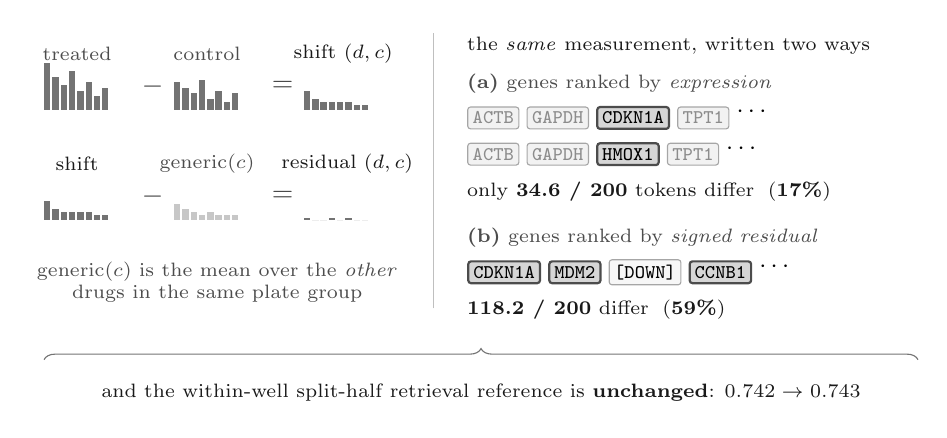
\begin{tikzpicture}[
  x=1cm, y=1cm, font=\small,
  bar/.style={fill=black!55, draw=none},
  faintbar/.style={fill=black!22, draw=none},
  gene/.style={draw=black!35, rounded corners=1pt, inner sep=1.8pt, font=\ttfamily\scriptsize},
  shared/.style={gene, fill=black!5, text=black!45},
  differs/.style={gene, fill=black!16, text=black, draw=black!70, thick},
  lbl/.style={font=\scriptsize, text=black!70},
  strong/.style={font=\scriptsize, text=black!90},
  op/.style={font=\normalsize, text=black!75},
]
\newcommand{\prof}[4]{%
  \foreach \h [count=\i from 0] in {#3} {
    \fill[#4] ($(#1,#2)+(\i*3.0pt,0)$) rectangle ++(2.3pt,\h pt);
  }%
}

% ================================================ LEFT: two subtractions
\node[lbl]    at (0.52,3.34) {treated};
\node[lbl]    at (2.17,3.34) {control};
\node[strong] at (3.90,3.34) {shift $\shift(d,c)$};
\prof{0.10}{2.62}{17,12,9,14,7,10,5,8}{bar}
\node[op] at (1.48,2.92) {$-$};
\prof{1.75}{2.62}{10,8,6,11,4,7,3,6}{bar}
\node[op] at (3.13,2.92) {$=$};
\prof{3.40}{2.62}{7,4,3,3,3,3,2,2}{bar}

\node[strong] at (0.52,1.94) {shift};
\node[lbl]    at (2.17,1.94) {generic$(c)$};
\node[strong] at (3.95,1.94) {residual $\resid(d,c)$};
\prof{0.10}{1.22}{7,4,3,3,3,3,2,2}{bar}
\node[op] at (1.48,1.52) {$-$};
\prof{1.75}{1.22}{6,4,3,2,3,2,2,2}{faintbar}
\node[op] at (3.13,1.52) {$=$};
\prof{3.40}{1.22}{1,0,0,1,0,1,0,0}{bar}

\node[lbl, anchor=north, align=center] at (2.30,0.82)
  {generic$(c)$ is the mean over the \emph{other}\\drugs in the same plate group};

\draw[black!25] (5.05,0.10) -- (5.05,3.60);

% ================================================ RIGHT: the encoding fork
\node[strong, anchor=west] at (5.35,3.44) {the \emph{same} measurement, written two ways};

\node[lbl, anchor=west] at (5.35,2.96) {\textbf{(a)} genes ranked by \emph{expression}};
\node[anchor=west] at (5.35,2.52) {%
  \tikz[baseline]{\node[shared]{ACTB};}\;\tikz[baseline]{\node[shared]{GAPDH};}\;%
  \tikz[baseline]{\node[differs]{CDKN1A};}\;\tikz[baseline]{\node[shared]{TPT1};}\;$\cdots$};
\node[anchor=west] at (5.35,2.06) {%
  \tikz[baseline]{\node[shared]{ACTB};}\;\tikz[baseline]{\node[shared]{GAPDH};}\;%
  \tikz[baseline]{\node[differs]{HMOX1};}\;\tikz[baseline]{\node[shared]{TPT1};}\;$\cdots$};
\node[strong, anchor=west] at (5.35,1.58)
  {only \textbf{34.6 / 200} tokens differ \;(\textbf{17\%})};

\node[lbl, anchor=west] at (5.35,1.00) {\textbf{(b)} genes ranked by \emph{signed residual}};
\node[anchor=west] at (5.35,0.56) {%
  \tikz[baseline]{\node[differs]{CDKN1A};}\;\tikz[baseline]{\node[differs]{MDM2};}\;%
  \tikz[baseline]{\node[gene, fill=black!3]{[DOWN]};}\;\tikz[baseline]{\node[differs]{CCNB1};}\;%
  $\cdots$};
\node[strong, anchor=west] at (5.35,0.08)
  {\textbf{118.2 / 200} differ \;(\textbf{59\%})};

% ================================================ the invariant
\draw[decorate, decoration={brace, amplitude=4pt}, black!55] (0.10,-0.55) -- (11.20,-0.55);
\node[strong, anchor=north] at (5.65,-0.73)
  {and the within-well split-half retrieval reference is \textbf{unchanged}: $0.742 \rightarrow 0.743$};

\end{tikzpicture}
\caption[The residual frame and the encoding fork]{\textbf{The information was always present; the
standard target's tokens barely expose it.} Left: the drug-specific residual is built by two
subtractions. The
control removes the cell's own state, leaving the \emph{shift}; the mean over the other drugs in the
same plate group removes the \emph{generic} programme that every compound triggers, leaving what
makes this drug different. Right: that same measurement, written two ways. Ranking genes by
expression (a) puts housekeeping genes first, so only $34.6$ of the top $200$ tokens differ between
two drugs in the same context; ranking by signed residual (b) raises that to $118.2$. (Divergence
counts quoted at cell-line scope, as in Table~\ref{tab:divergence}; plate scope is similar.) The
bracket is the point of the figure --- the within-well split-half retrieval reference is essentially
identical under both encodings, so no information has been added. What changed is how much of it the
token sequence exposes to the loss --- a property of the encoding, which is not the same as showing
the encoding is what binds (Table~\ref{tab:divergence}).}
\label{fig:frame}
\end{figure}


\begin{claim}
Ranking the target by signed residual exposes $59\%$ of its top-$200$ gene positions to the drug at
cell-line scope, and $60\%$ at the plate scope this build actually uses, against $17\%$ for the
standard target (Table~\ref{tab:divergence}), at an unchanged within-well split-half retrieval
reference; and the residual is estimable
without leaking the evaluation into the fit --- split before fit, generic plate-scoped and
drug-meaned, reliability resolved from the data at the matched null's $95$th percentile
($+0.109$). That is a statement about the fitting procedure and not about plate structure, which
the paragraph above leaves measured only in expectation. What that establishes is that the
standard target's tokens hide a difference the data contain --- and that this is a fact about
ranking genes on absolute expression rather than a fact about these drugs, since $92\%$ of the
recoverable between-drug difference returns as soon as the cell's own control is subtracted. It
does not establish that tokenisation is the binding constraint: the residual package changes five
things at once, listed in full above.
\end{claim}

\subsection{How much signal is there to encode}
\label{sec:methods-vardecomp}
\label{sec:res-transfer}

The residual defines what the model should predict. Before reporting what happened when a model was
trained on it (\S\ref{sec:res-encoding}), this section measures the target itself --- how much
drug-specific signal it carries, and of what kind --- because the same training result reads
differently against a large reachable signal and against a small one.

The shift's energy decomposes exactly into residual $0.621$, generic $0.390$ and a cross term of
$-0.011$: $62.1\%$ of the perturbation response's energy is drug-specific, $39.0\%$ is the generic
programme, and the two components are essentially orthogonal, so the shares are genuine
(\texttt{vardecomp\_matched.json}). Put that number beside Table~\ref{tab:divergence} and the
encoding problem states itself in one line: the drug-specific part is the majority of the
perturbation response, $62.1\%$ of its energy, and two drugs in the same context still share $83\%$
of the top-$200$ genes in the standard target. The drug is not a small effect in the response. The
response is not what a cell sentence ranks. Every claim that follows is scoped by the first of those
numbers, and it has not previously been computed for this task. Its frame is not quite the
trained-on one: the stored generic averages over conditions and keeps the condition's own
contribution, where the training frame of \S\ref{sec:methods-residual} averages over drugs and
leaves the condition's own drug out. Self-inclusion scales a residual by $(m-1)/m$ in a plate group
of $m$ conditions, so that difference depresses the share quoted here rather than inflating it; the
weighting difference has no established direction.

Within the drug-specific part, two components call for different responses. Modelling
\begin{equation}
 \resid(d,c) \;=\; \beta(d) \;+\; \kappa(d,c) \;+\; \epsilon,
 \qquad
 \Tcoef \;=\; \frac{\operatorname{var}\beta}{\operatorname{var}\beta + \operatorname{var}\kappa},
\end{equation}
the per-drug constant $\beta(d)$, the drug \emph{main effect}, is retrievable without any
model: it is what a lookup table reproduces. The remainder $\kappa(d,c)$ is the only component a
conditional model could win on. It is written here as a drug$\times$cell-line interaction because
that is what the decomposition assumes; the estimator actually used does not identify such a term,
for the reasons set out below, so $\kappa$ is called the \emph{context-specific remainder} and
$\Tcoef$ a disattenuated cross-context residual-similarity coefficient rather than a variance
share. The decomposition's additive part is what remains identified. This is DrEval's naive predictor, in
transcriptomic space: their \texttt{NaiveMeanEffectsPredictor}~\cite{dreval} predicts
$\hat{y}_{ij} = \mu^c_i + \mu^d_j - \mu$, an additive model of cell-line and drug main effects with
no interaction term, and our $\textrm{generic}(c) + \beta(d)$ is precisely that quantity lifted from
a scalar potency to a $946$-dimensional profile. It follows that $\kappa$ is the term their naive
model omits. It does not follow that $1 - \Tcoef$ measures the headroom available above it: the
cross-line pairs entering $\Tcoef$ may also differ in dose and in treatment well, and each
condition's residual is taken against a generic its own drug helped define, so $1 - \Tcoef$ bounds
that headroom from above at best. DrEval finds
that deep models barely beat this additive baseline on drug sensitivity; the transfer coefficient
asks whether, in the transcriptomic setting, there is anything above it to win in the first place.

$\Tcoef$ is estimated by disattenuated cross-line correlation rather than by fitting the
variance-components model directly, for a reason this cache's layout forces: with $286$ of $287$
treatments in exactly one well there is no replicate from which to separate
$\operatorname{var}\kappa$ from $\operatorname{var}\epsilon$, so the decomposition is unidentified
on its own. The cosine route buys identification through split-half reliability:
\begin{equation}
 \hat{\Tcoef} \;=\; \frac{\cos\!\big(\resid(d,c_1),\, \resid(d,c_2)\big)}
 {\sqrt{\rho(d,c_1)\,\rho(d,c_2)}},
 \qquad
 \rho(d,c) \;=\; \frac{2\cos(\resid_A, \resid_B)}{1 + \cos(\resid_A, \resid_B)},
\end{equation}
where $\resid_A$ and $\resid_B$ are disjoint halves of condition $(d,c)$ and $\rho(d,c)$ is the
Spearman--Brown reliability of its full-sample residual. Two cautions attach, and both are stated
where the numbers live. Dividing out the reliability, the disattenuation, is essential:
measurement noise alone depresses the raw cross-line cosine and would otherwise be read as
interaction. And the correction is a Spearman--Brown formula applied to a cosine, though it is
derived for correlations between parallel halves; the planted-truth validation of
Appendix~\ref{sec:app-planted} is what licenses it empirically. The reliability entering it is a
within-well split-half precision, optimistic relative to true biological reproducibility. That
optimism sits in the denominator: an over-large $\rho$ makes $\hat{\Tcoef}$ too small, so the
unshared fraction $1 - \hat{\Tcoef}$ is, if anything, \emph{overstated}. An earlier draft of this
section had the direction the wrong way round.

The measurement itself carries a control-design lesson, stated because it changed the protocol. The
first run compared $\Tcoef$ against a negative control of different drugs on the same plate, which
returned $+0.485$ against $\Tcoef = 0.511$, and was correctly declared void: that control differs
from the estimand in two ways at once, different drug and same cell line, and plate structure
surviving a cell-line-scoped generic inflates same-plate comparisons (the $+0.485$ just quoted,
against a separate $-0.017$ plate-scoped diagnostic, which is voided rather than matched) while leaving
cross-line comparisons untouched. A structure-matched control --- different drug, different cell
line, breaking only the drug match --- is the one that bounds the estimand, and a negative control
that differs in more than one way cannot do so. Five checks in all accompany the estimate, and
Table~\ref{tab:tcontrols} states what each bounds.

\begin{table}[htbp]
\centering
\footnotesize
\begin{tabularx}{\textwidth}{@{}>{\raggedright\arraybackslash}p{0.30\textwidth}X@{}}
\toprule
Check & What it bounds \\
\midrule
disjoint control halves & shared-control inflation: $+0.242$ at cell-line scope, $-0.000$ at plate \\
structure-matched negative control & the estimand itself; returns $-0.008$ \\
simulated $\kappa{=}0$ null & estimator bias: returns $1.001$ where the truth is $1.000$ \\
dose strata on molar doses & a reference scale: the same drug and line at another dose \\
leave-one-drug-out generic & train/held-out target asymmetry (\S\ref{sec:methods-residual}) \\
\bottomrule
\end{tabularx}
\caption{The five checks accompanying the transfer-coefficient estimate. The simulated null matters
most: at $\kappa = 0$ the \emph{uncorrected} cross-line cosine is only $0.734$, which read naively
reports $27\%$ interaction where the truth is zero, while the disattenuated estimator recovers the
truth to within $0.001$. That recovery is what licenses the reference column below. The dose strata carry a molar-resolved dose --- an earlier
cache carried the well identifier in the dose field, so what was labelled dose transfer compared
physical samples rather than concentrations.}
\label{tab:tcontrols}
\end{table}

\begin{table}[htbp]
\centering
\footnotesize
\begin{tabularx}{\textwidth}{@{}>{\raggedright\arraybackslash}p{0.30\textwidth}
  >{\centering\arraybackslash}p{0.10\textwidth}
  >{\centering\arraybackslash}p{0.18\textwidth}X@{}}
\toprule
Quantity & Estimate & 95\% interval & Reference \\
\midrule
$\Tcoef$ (cross-context, plate-scoped generic) & $0.553$ & $[0.514, 0.593]$ & simulated $\kappa{=}0$ null $= 1.001$ \\
similarity scale NOT shared across contexts, $1-\Tcoef$ & $44.7\%$ & $[40.7\%, 48.6\%]$ &
mixes cell line, dose, well and estimator \\
$\Tcoef$ across dose (same drug, same line) & $0.707$ & $[0.632, 0.782]$ & reference scale \\
structure-matched negative control & $-0.008$ & spanning zero & must be $\approx 0$ \\
\bottomrule
\end{tabularx}
\caption{The transfer coefficient, estimated on real molar doses with dyadic cluster-robust
intervals. The matched negative control sits on zero; the same-plate control that produced the
earlier false alarm reads $+0.485$ under a cell-line-scoped generic, for the reasons given in the
text. $\Tcoef$ is a cross-context similarity coefficient, not a variance share, and $1 - \Tcoef$
must not be read as a drug$\times$cell-line interaction share.}
\label{tab:transfer}
\end{table}

$\Tcoef$ is a descriptive sensitivity analysis, not a load-bearing estimate, and the reason is in
its own configuration. The scoped calculation retains conditions at a reproducibility threshold of
$0.2$; it permits cross-line pairs that differ in \emph{dose} (\texttt{same\_dose\_only=false}); it
uses a \emph{self-including} generic (\texttt{loo\_generic=false}), so each condition's own drug
contributes to the programme subtracted from it; and a cross-line pair may also sit in a different
treatment well. What the number is, precisely, is a disattenuated cross-context residual-similarity
coefficient over pairs that differ in cell line, dose, well and target estimator at once:
$\Tcoef = 0.553$ \nolinebreak[3]$[0.514, 0.593]$, so $44.7\%$ $[40.7\%, 48.6\%]$ of that similarity
scale is not shared across the compared contexts. Its one useful asymmetry is directional: for the reason
given above, an optimistic reliability in the denominator pushes $\hat{\Tcoef}$ down, so
$1 - \Tcoef$ errs high and bounds from above what a per-drug constant leaves on the table rather
than measuring it.

One contrast in this analysis comes close to varying a single factor, and it deserves stating as a
result rather than spending as a check. Holding drug and cell line fixed and changing only the molar
concentration, transfer is $0.707$ $[0.632, 0.782]$ on $363$ pairs, against $0.553$ $[0.514, 0.593]$
for the pooled cross-context comparison; the two intervals do not overlap. Dose is the milder
perturbation of a drug's residual. The ordering is between one clean axis and a mixture rather than
between dose and cell line alone --- the cross-context arm differs in well and in dose as well as in
cell line --- but the dose arm is the closest this section comes to a single-axis contrast: drug and cell line
are fixed, and only the well necessarily moves with the dose.

That ordering also did duty as a diagnostic when the generic's scope was chosen, and it is the
weaker of the two that were used. At cell-line scope it inverts: the dose arm falls to $0.4846$ ---
a different quantity from the voided same-plate control above, which coincidentally reads $0.4853$
--- while the cross-line coefficient holds at $0.511$ (\texttt{vardecomp\_baseline.json}), which is the wrong
way round for what one expects of dose against cell line. But that expectation is a prior rather
than anything measured here, so the argument is a plausibility check and is used as one. The second
diagnostic needs no prior. At plate scope the shared-control and split-control builds of $\Tcoef$
agree to $-0.000$; at cell-line scope they differ by $+0.242$, which is plate structure leaking
through a cell-line-scoped generic and inflating same-plate comparisons. That is what the scope
decision rests on, and it is also why the cell-line-scoped build cannot be offered as corroboration
when it returns a similar $\Tcoef = 0.511$: that build is the one declared void above, its own
same-plate negative control reading $+0.485$.

The per-drug constant $\beta(d)$, which the lookup of \S\ref{sec:res-lookup} reproduces almost
exactly, is therefore not the whole signal. What it cannot express is the part that does not
transfer across contexts --- a quantity that, for the reasons given above, does not isolate a
drug$\times$cell-line interaction, and no size for one is estimated here.

Whether anything could learn that interaction is a separate question. If a cell line modulated drug
responses in a consistent direction, that direction would be estimable from the line's own cells and
a conditional model would have a concrete target. Writing $\kappa(d,c) = \resid(d,c) -
\hat{\beta}(d)$, the test compares $\cos(\kappa(d,c), \kappa(d',c))$ for different drugs in the same
cell line against the same quantity across different cell lines, with $\hat{\beta}$ estimated
leave-one-cell-line-out: estimated over all lines it would contain $\resid(d,c)$ itself, and
subtracting a mean containing its own term induces a $-1/(m-1)$ correlation that biases the signal
arm downward by construction, which would make a structured interaction look idiosyncratic --- the
exact error the test exists to avoid. Both arms are disattenuated by $\kappa$'s own split-half
reliability, since $\kappa$ is a difference of two noisy quantities and is therefore noisier than
the residual it comes from.

\begin{table}[htbp]
\centering
\footnotesize
\setlength{\tabcolsep}{4pt}
\begin{tabular}{lrrr}
\toprule
Configuration & same cell line & different cell lines & excess within-line \\
\midrule
plate-scoped generic & \ci{-0.0149}{-0.0251}{-0.0050} & \ci{+0.0003}{-0.0071}{+0.0081} & $-0.0153$ \\
\bottomrule
\end{tabular}
\caption{No cell line bends different drugs in a consistent direction. Both entries are
disattenuated by $\kappa$'s own split-half reliability, and their intervals come from a
cell-line-clustered bootstrap ($38$ and $42$ clusters). $4{,}000$ pairs in the same-line arm and
$3{,}884$ across lines, over $1{,}282$ conditions (\texttt{vardecomp\_matched.json}). The
same-line interval lies entirely below zero, so the arm that would have to be positive for a
per-cell-line direction to exist is not merely null. The excess is the difference of the two
point estimates; no interval was computed for it. A cell-line-scoped counterpart was not
computed in the canonical run and the row an earlier draft carried for it is withdrawn.}
\label{tab:kappa}
\end{table}

We looked for structure in $\kappa$ and did not find it: no cell line modulates different drugs in
a consistent direction, and a direct test of whether mechanism-matched drugs deviate from their
per-drug constants in the same way within a given cell line returned nothing detectable.
 The temptation is to read two negative results as irreducibility, and they do not
support it. The second test bounds its own power severely: $\kappa$'s split-half reliability in this
atlas is $0.195$ at the $0.05$ reliability floor ($0.324$ at the stricter $0.20$ floor), so the
quantity being correlated is barely estimable, and same-mechanism compounds are so heavily co-plated
that only $3$--$7\%$ of matched pairs survive a different-plate requirement ($1\%$ at the stricter
floor), which leaves the plate confound in place. The defensible reading is that $\kappa$'s
structure is unresolved in this dataset. Resolving it would take more cells per condition, or a
plating design that crosses mechanism with plate --- neither of which is an analysis choice.

\begin{claim}
There is a conditional target that a per-drug constant cannot express. Two tests looked for learnable
structure in it and found none, and neither settles whether there is any --- $\kappa$'s split-half
reliability is $0.195$ at the floor the mechanism test runs at, and only $3$--$7\%$ of
mechanism-matched pairs survive a different-plate requirement --- so its structure is unresolved here
rather than shown to be absent. Its size is quoted as what it is: $\Tcoef = 0.553$ \nolinebreak[3]$[0.514, 0.593]$ is a
disattenuated cross-context similarity coefficient, so $44.7\%$ of \emph{that similarity scale}
remains unshared across the compared contexts. It is not a variance share and not a
drug$\times$cell-line interaction --- the estimator pools pairs differing in cell line, dose, well
and target estimator --- so it bounds what a per-drug constant leaves on the table without
establishing that a model could reach any of it.
\end{claim}

\subsection{Re-encoding produces prompt sensitivity}
\label{sec:res-encoding}

Re-encoding the target as the drug-specific residual raises the differing fraction to $59\%$ at
cell-line scope --- $60\%$ at the plate scope this arm is trained in --- at an unchanged within-well
split-half retrieval reference, and the model trained on it responds to the drug it is told about. On
the $300$ trained conditions of the residual-frame evaluation it beats the geometry-defined
\texttt{orth} scrambled partner, whose observed score is empirically near chance, by
\ci{+0.0898}{+0.0291}{+0.1506}, clustered on the drug and the treatment well, the drug
being the axis a claim about drugs has to survive (\texttt{re\_v3.json};
Table~\ref{tab:generalisation} sets this beside the held-out splits, and the two instruments that
need no comparator arm at all are read below). That is the first non-null drug effect in this
project --- first in the order the experiments were run, and, as the budget-matched re-run below
shows, not the only target construction that produces one.

The gradient that first exposed the effect is worth stating in its own terms. On the earlier target
build, the stratified scramble of \S\ref{sec:methods-controls} gave a gap that grew with swap
dissimilarity --- \ci{+0.0351}{+0.0061}{+0.0656}, \ci{+0.0716}{+0.0371}{+0.1059} and
\ci{+0.1429}{+0.1112}{+0.1787} across the \texttt{near}, \texttt{orth} and \texttt{opposite}
strata, each model score differenced against its own stratum-specific partner. Thus $+0.0716$ is
the \texttt{orth} gap and $+0.1429$ is the \texttt{opposite} gap. Each gap uses its own
stratum-specific partner. Those partners score $0.550$, $0.501$ and $0.423$ across
\texttt{near}, \texttt{orth} and \texttt{opposite}: both \texttt{near} and \texttt{opposite}
differ from chance in opposite directions, while \texttt{orth} is empirically near chance in this
sample. The monotone ordering is itself the evidence: a metric artefact would not order itself by
swap dissimilarity. The series is therefore quoted as a gradient, while the \texttt{orth} magnitude
is the least contaminated available comparison --- not an independently established null, because
the stratum itself was defined using true residual geometry. The second qualification is that these are
the residual arm's $1400$-token run, while the two control arms plotted beside them were scored at
the $600$-token cap of \S\ref{sec:methods-data}, where their stratum gaps run from $-0.021$ to
$+0.026$ (\texttt{fig-repair.json}). Those controls were read at the time as flat and null at every
stratum. That is true of the single-cell arm, at $600$ tokens and again at the residual arm's
budget. It is not true of the optimal-transport arm, whose $600$-token gaps are themselves monotone
in swap dissimilarity, and which does not stay flat once it is given the residual arm's budget, as
the re-run below establishes.

\begin{figure}[htbp]
\centering
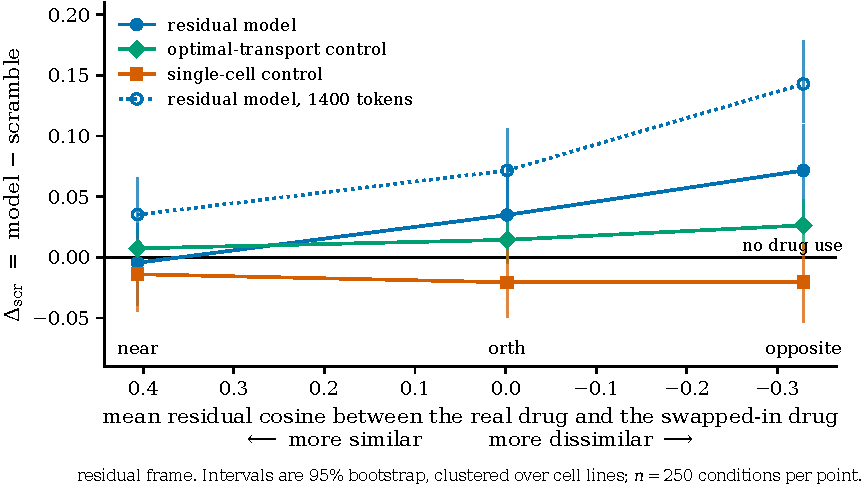
\includegraphics[width=\textwidth]{fig-repair}
\caption[The gap grows with swap dissimilarity]{\textbf{On the earlier target build, the residual
model's advantage over its own scramble grew with how dissimilar the swapped-in drug's response was;
the single-cell control scored through the identical pipeline stayed flat and null, while the
optimal-transport control did not --- its $600$-token gaps are themselves monotone, and at the
residual arm's budget against the geometry-defined \texttt{orth} partner, whose observed score is
near chance, they clear zero (text).} The horizontal axis is the
measured mean residual cosine between the real and swapped-in drug, which is byte-identical across
all four runs, so the positions are exact. The three solid series are at a matched $600$-token
generation budget; the residual model's $1400$-token run is drawn separately as the dotted overlay,
since the budget alone roughly doubles the gap on the two strata where it is positive at $600$
($+0.0349 \rightarrow +0.0716$ on \texttt{orth}, $+0.0716 \rightarrow +0.1429$ on
\texttt{opposite}). Intervals are $95\%$ bootstrap clustered over cell lines,
$n=250$ conditions per point. The \texttt{near} stratum is the weakest test by construction: where
the swapped-in drug's true response is similar, an unchanged output is correct rather than blind.}
\label{fig:repair}
\end{figure}

Three further diagnostics on that build agreed, and the residual model led on all three --- it won
outright on reproducibility association and prediction diversity, and had the largest
own-versus-other cosine margin on the third, although all three arms passed that cosine diagnostic. The
correlation between condition reproducibility ($\textrm{repro\_cos}$, the condition's split-half
residual cosine) and model $\NIR$ was $+0.144$ --- the model does better where the drug effect is
real, against $-0.117$ and $-0.216$ for the controls. Prediction diversity was highest for the
residual model. And while $\cos(\textrm{prediction}, \textrm{own truth})$ exceeded
$\cos(\textrm{prediction}, \textrm{other drugs})$ for all three arms, the residual model's margin
($+0.084$) was roughly twice the optimal-transport arm's ($+0.049$) and three times the single-cell
arm's ($+0.026$).

One measurement lesson and one withdrawal belong with this result. The effect was first measured at
the $600$-token generation cap of \S\ref{sec:methods-data}, which roughly halved it at every
stratum where it was positive there: on \texttt{opposite} the gap reads $+0.0716$ at $600$ tokens
against $+0.1429$ at $1400$, and on \texttt{orth} $+0.0349$ against $+0.0716$. The value $+0.0716$
therefore appears twice in this section --- once as the $600$-token \texttt{opposite} gap and once
as the $1400$-token \texttt{orth} gap quoted above --- and the two are not the same quantity.
Both controls have since been re-run at the residual arm's $1400$-token
budget, and the result narrows this section's claim rather than confirming it. The single-cell
control stays flat, as it was at $600$: $-0.0128$ \nolinebreak[3]$[-0.0458, +0.0202]$ against its
own geometry-defined \texttt{orth} partner, spanning zero. The optimal-transport control does \emph{not}. At $600$
tokens its gap was $+0.0144$ \nolinebreak[3]$[-0.0051, +0.0338]$ and spanned zero; at $1400$ it is
$+0.0292$ \nolinebreak[3]$[+0.0144, +0.0441]$ and does not. The token budget was suppressing a real
effect in that arm, which is the same lesson the residual arm taught, applied to a control that was
previously read as inert.

The comparison that decides the matter is between the two arms' own gaps, and it costs this section
its strongest phrasing. The residual arm's pooled gap against its geometry-defined \texttt{orth}
partner is
$+0.0361$ \nolinebreak[3]$[+0.0159, +0.0564]$ over $1{,}394$ conditions; the optimal-transport arm's,
at the same budget, is $+0.0292$ \nolinebreak[3]$[+0.0144, +0.0441]$ over $248$
(\texttt{ctrl1400\_summary.json}). Those intervals overlap almost entirely. Re-encoding
the target therefore produces prompt sensitivity, but it is \emph{not} the only target change that
does, and the claim that it produced the first non-null effect in the project holds in the
order the experiments were run, not as a statement that the residual encoding is uniquely
responsible. Three limits bound the comparison in the other direction: the arms are scored in
different frames, so their absolute $\NIR$s are not comparable and only each arm's gap against its
own comparator is; they are separate evaluations over different condition sets, so this is an
arm-level comparison and not a paired one; and those two condition sets differ in split composition
by more than the arms differ from each other. The residual figure pools $300$ trained, $895$
unseen-combination and $199$ unseen-drug conditions, whose own gaps are $+0.0898$, $+0.0332$ and
$-0.0315$; the optimal-transport evaluation carries no split labels at all, so its $248$ conditions
cannot be sorted into trained and held-out. A spread of that size across splits, against a $0.0069$
difference between the two pooled numbers, means the near-equality does not order the arms in
either direction.

``OT achieved nothing'' is therefore withdrawn, and not weakly. The optimal-transport arm's
$1400$-token gap is measured against a partner whose true response is on average orthogonal to the
target's ($\cos = +0.035$), the least contaminated available stratum because its observed score is
empirically near chance; the geometry-based selection does not independently establish a null. The
$600$-token evidence pointed the same way and was
read too cautiously: the arm's stratum gaps there were $+0.0073$, $+0.0144$ and $+0.0263$, monotone
in swap dissimilarity like the residual arm's, with only the \texttt{opposite} stratum excluding
zero. That gap cannot supply a clean magnitude: the \texttt{opposite} comparator scores below
chance, while the \texttt{near} comparator scores above it; only the geometry-defined
\texttt{orth} partner is empirically near chance in this sample. What the matched
budget supplies is the \texttt{orth}-partner reading, and it clears zero. The consequence reaches
backwards: the optimal-transport target is a point in the three-point comparison of
\S\ref{sec:res-epsilon}, whose negative holds only at the budget and comparator it was
measured with. At a matched budget and the geometry-defined \texttt{orth} partner, whose score is
empirically near chance, the optimal-transport point is not null; the
single-cell point is the one whose interval still spans zero.

The comparator-free evidence is already in hand: regressing
each generation's $\NIR$ on the cosine between the named drug's truth and the target's truth gives a
slope of \ci{+0.3728}{+0.2797}{+0.4660} on trained conditions. Zero slope is the natural null,
so no comparator defect can reach it --- though the regression's points are the three scrambled
partner prompts and nothing else, and the target-drug prompt is never one of them, which bounds what
it says (\S\ref{sec:res-generalisation}). Re-encoding the target made the model respond to the combined
drug-and-mechanism prompt. What that response is worth is the question the rest of the chapter
answers.

\begin{claim}
Re-encoding the target produced the project's first non-null drug effect. On trained
conditions the model beats the geometry-defined \texttt{orth} partner by
\ci{+0.0898}{+0.0291}{+0.1506} and beats chance
outright --- with no comparator arm at all --- by \ci{+0.0981}{+0.0407}{+0.1554}, both clustered on
the drug and the treatment well, the drug being the axis the claim rides on
(\S\ref{sec:res-generalisation}).
The comparator-free slope of retrieval against the named drug's truth is
\ci{+0.3728}{+0.2797}{+0.4660} --- zero is its natural null, so no comparator defect can reach it,
though it is fitted over the scrambled partner prompts alone, with the target-drug prompt never a
point on the line.
It is first in sequence and not uniquely responsible: at a matched $1400$-token budget the
optimal-transport target clears zero against its own \texttt{orth} partner too
(\ci{+0.0292}{+0.0144}{+0.0441} over $248$ conditions that carry no split labels, against the
residual arm's \ci{+0.0361}{+0.0159}{+0.0564} pooled over $1{,}394$ that mix trained and held-out
splits), on a separate evaluation in a different frame --- so the two are not ordered against each
other.
Sensitivity is established; fidelity is the next question.
\end{claim}

\subsection{Sensitivity is not fidelity}
\label{sec:methods-holdout}
\label{sec:res-generalisation}

A model that responds to the drug token has cleared a low bar, because reproducing a training
average requires responding to it too. Everything scored above came from conditions the model
trained on, so the result so far shows that the token is consulted --- not that anything
transferable was learned. Separating those two requires withholding data, and the physical layout of
\S\ref{sec:methods-data} forces which withholding is meaningful. A (drug, cell line) holdout ---
the field's standard Leave-Pairs-Out split, and the split an earlier version of this work used ---
leaves the held-out condition's treated well sitting in the training set through its other
$\approx 48$ cell lines. Measured against the holdout this investigation previously used, $124$ of
the $255$ treated wells for which split information exists placed a held-out condition and a
training condition in the same physical sample. What that estimand measures is within-atlas matrix completion, not independent
generalisation, and no processing of the targets changes it, because it is a property of what was
randomised.

Holding out whole wells is the only assignment-respecting choice the design offers, and it answers a
different and narrower question: generalisation to an unseen treatment well of a seen drug --- a new
physical preparation, not a new cellular context. Fixed-dose cross-context transfer, present in one
line and absent in another, is structurally unidentifiable in this atlas; this is a property of
Tahoe's design, not of our pipeline, and no rebuild fixes it.

The split used throughout the residual arm is therefore keyed at the well. \texttt{train} holds
every condition of the remaining wells ($4{,}999$ conditions before the reliability line, $2{,}523$
after it). \texttt{unseen\_combo} holds $36$ treated wells out whole ($904$ conditions, $900$ after
inventory filters), and the holdout never takes a drug's last training well --- without that guard a
two-well drug could silently become an unseen drug while sitting in the unseen-combination arm,
making the two arms measure the same thing; zero wells contribute conditions to both sides of this
split. \texttt{unseen\_drug} holds every condition of $10$ held-out drugs ($714$ conditions, $711$
after inventory filters): Tahoe fine-tuning never sees the token, so this is the control --- though
the Pythia-1b backbone was pretrained on natural language and the prompt still supplies the
\texttt{Mechanism:} field, so ``unseen'' means held out from fine-tuning with mechanism supplied, not
unknown to the pipeline. A large effect there would indict the comparator rather than report a
biological finding. We do not build a Leave-Cell-Lines-Out
split here; Section~\ref{sec:limitations} argues it is the natural next axis and explains why its
interest is contingent on the transfer coefficient. Two warnings ride with the design. DrEval
reports, citing~\cite{partin}, that apparently good performance on pair-holdout splits can be
reached simply by predicting each drug's average response across the training cell lines; our
held-out-well estimand sits exactly in the regime where that warning bites, which is why the
baseline ladder of \S\ref{sec:res-lookup} is not optional --- the drug-average predictor is not a
formality, it is the hypothesis under test. And evaluation samples conditions under an explicit
per-split quota, because a uniform draw reproduces the pool's proportions and starves precisely the
split the experiment exists to test: in a first run, $250$ constructed held-out combinations yielded
only $33$ scored conditions, purely as an artefact of the sampler. The residual-frame evaluation
therefore scores $300$ train, $895$ \texttt{unseen\_combo} and $199$ \texttt{unseen\_drug}
conditions, $1{,}394$ in all --- the \texttt{unseen\_combo} arm now takes almost the whole pool of
$900$, while \texttt{unseen\_drug} remains a quota of the $711$ available, so that verdict is
powered on a subset of the conditions the split affords and its detection limit should be read with
that in mind.

The first result from this design is about the comparator, and it is a finding rather than an
erratum: it reframes every gap quoted so far. The comparator's own score gives it away. Across the
three swap strata the scrambled model's $\NIR$ is $0.550$, $0.501$ and $0.423$ as the named
partner's true response moves from aligned ($\cos = +0.22$) through orthogonal ($0.00$) to
anti-aligned ($-0.20$) with the target (\texttt{re\_v3.json}). A comparator whose own score is a
monotone function of which drug it was handed is not a null: it is an active treatment that tracks
the partner drug. Both the \texttt{near} score of $0.550$ and the \texttt{opposite} score of $0.423$
differ from chance in opposite directions; the geometry-defined \texttt{orth} partner scores
$0.501$ and is empirically near chance in this sample. That observation makes \texttt{orth} the
least contaminated available comparator, not an independently established null: its stratum was
defined using true residual geometry. The swap partner is itself a drug the model was mostly trained on, so
telling the model a lie costs it precisely because it knows the partner. A gap measured against such
an arm decomposes as
\begin{equation}
 \gap \;=\; \underbrace{\big(\NIR_{\textrm{model}} - 0.5\big)}_{\textrm{how much naming the truth helps}}
 \;+\; \underbrace{\big(0.5 - \NIR_{\textrm{scramble}}\big)}_{\textrm{how much naming the lie hurts}},
\end{equation}
and only the first term is wanted. The second term is not a rounding error. Pooled over all
$1{,}394$ scored conditions the model's own advantage over chance is $+0.0367$ and the
\texttt{opposite} comparator's deficit is $+0.0772$: $68\%$ of the $+0.1139$ gap that arm reports is
the comparator failing, not the model knowing. Against \texttt{orth}, whose own score is empirically
near chance ($0.501$), the second term is approximately zero in this sample. Every gap in
Table~\ref{tab:generalisation} is therefore measured against that geometry-defined partner, and its
magnitude is conditional on the observed near-chance score rather than licensed by an independent null; the
\texttt{opposite} figures are quoted in prose below, solely as the diagnostic that would have misled
us.

The diagnostic is free and it is not specific to this experiment: score the comparator arm against
chance, and if its score moves with which label it was handed, the gap it defines is not a
measurement of the model. That condition is easy to meet by accident. A swap drawn to be maximally
dissimilar --- the obvious way to build a strong negative control --- is exactly the swap that
maximises the second term, so the harder the control is made to look, the more of the reported gap
belongs to it rather than to the model.

\begin{table}[htbp]
\centering
\resizebox{\textwidth}{!}{%
\begin{tabular}{lrrll}
\toprule
Split & $n$ (lines; drugs; wells) & model $\NIR$ & $\gap$, clustered on \emph{cell line} & the same, clustered on \emph{drug} \\
\midrule
\texttt{train} & 300 (39; 76; 136) & 0.598 [0.549, 0.647] & \ci{+0.0898}{+0.0382}{+0.1415} & \ci{+0.0898}{+0.0291}{+0.1506} \\
\textbf{\texttt{unseen\_combo}} & \textbf{895 (42; 34; 36)} & \textbf{0.533 [0.492, 0.575]} & \ci{+0.0332}{+0.0069}{+0.0594} & $+0.0332$ [$-0.0031$, $+0.0695$] \\
\texttt{unseen\_drug} & 199 (40; 10; 28) & 0.459 [0.404, 0.514] & $-0.0315$ [$-0.0836$, $+0.0206$] & $-0.0315$ [$-0.1049$, $+0.0419$] \\
\bottomrule
\end{tabular}}
\caption{Whole-well holdout on the corrected evaluation --- the truth verified against the build's
own fit digest, and the full held-out population rather than the reliability-surviving subset. The
two right-hand columns carry the SAME point estimate and differ only in what they treat as the unit
of generalisation. On \texttt{train} the gap excludes zero either way. On \texttt{unseen\_combo} it
excludes zero clustered on cell line and does not clustered on drug --- which, for the reason the
text below gives, is why this row is reported as not established. Every gap printed here is measured
against the geometry-defined \texttt{orth} partner, whose own score is empirically near chance in
this sample; \texttt{opposite} figures
never appear as a column here. The
\texttt{unseen\_drug} row corroborates rather than proves: those drugs were held out of Tahoe
fine-tuning, so a large gap there would indict the comparator --- but the base model was pretrained
on natural language and the prompt still supplies a mechanism, so a strictly zero effect was
never guaranteed. Its \texttt{orth}-partner gap is negative ($-0.0315$) while its \texttt{opposite} gap is
$+0.0379$: the same comparator asymmetry the other two rows show.
What establishes comparator non-neutrality is the direct $0.550/0.501/0.423$ ordering above.
Model $\NIR$ intervals test against the chance value $0.5$ with no comparator. Intervals are two-way
cluster-robust over cell lines and wells, with a Student $t$ reference on $\min(G_{\textrm{line}},
G_{\textrm{well}}) - 1$ degrees of freedom --- which is why the well counts are printed: the
\texttt{unseen\_drug} arm spans $28$ wells, and $t_{27} = 2.05$ against $1.96$ widens its interval by
five per cent (\S\ref{sec:methods-data}).}
\label{tab:generalisation}
\end{table}

The control behaves exactly as the diagnosis predicts. On \texttt{unseen\_drug} --- drugs held out
of Tahoe fine-tuning, though not of the base model's pretraining, and with the mechanism still
supplied in the prompt --- the gap against \texttt{opposite} is $+0.0379$
\nolinebreak[3]$[-0.0083, +0.0841]$, positive where the \texttt{orth}-partner estimate is negative. The same
conditions, the same generations and the same model scored against the geometry-defined
\texttt{orth} stratum give
$-0.0315$ \nolinebreak[3]$[-0.0836, +0.0206]$, an interval that covers zero as a control should ---
though the point estimate is negative and of the same size as the \texttt{unseen\_combo} gap with
the sign reversed, so this row is read as uninformative rather than as a confirmed null. The
interval on the \texttt{opposite} arm is itself a lesson in the inference regime: a cluster-robust
variance is asymptotic in the number of clusters rather than observations, and this arm spans $40$
cell lines but only $28$ treatment wells, so the two-way variance is carried on $27$ degrees of
freedom. A cell-line-only cluster bootstrap puts the gap clear of zero at $[+0.0044, +0.0727]$;
adding wells as the second clustering axis, as every interval in Table~\ref{tab:generalisation}
does, returns it to zero, and it does so at the normal quantile as well as at $t_{27} = 2.05$. What
decides this row is the unit of clustering, not the quantile.

Read against the geometry-defined \texttt{orth} partner, \texttt{train} clears zero under either clustering
(\ci{+0.0898}{+0.0382}{+0.1415} on cell line and well; $[+0.0291, +0.1506]$ on drug and well).
On \texttt{unseen\_combo} the point estimate is $+0.0332$: its interval is
$[+0.0069, +0.0594]$ clustered on cell line and well and $[-0.0031, +0.0695]$ clustered on drug and
well, so it clears zero under only one of the two units the claim needs. Drug is the axis a claim about
transferring a \emph{drug} signature has to generalise across, so generalisation to an unseen
treatment well of a seen drug is not established. The split is also weaker than its name: $30$ of
its $34$ drugs and $39$ of its $42$ cell lines appear in training, and $82\%$ of its conditions
recombine a seen drug with a seen cell line; and what positive effect there is is a majority tilt
rather than a uniform one, positive for $20$ of the $34$ drugs (sign test $p = 0.39$). The precision matters: not established
is not the same as shown to be zero. The drug-clustered interval reaches $+0.0695$, so an effect of
up to roughly $+0.07$ remains compatible with these data at $n = 895$ spread over $34$ drugs --- a
limit of power at the sample size the holdout affords, reported as one. (On \texttt{unseen\_drug},
$n = 199$ leaves a half-width of $0.055$ around the model's own $\NIR$ and an $80\%$-power detection
limit of $0.079$ against chance.) The three splits are not scored on comparable populations. Their
raw within-well split-half precision references are $0.956$, $0.824$ and $0.836$, a spread of
$0.132$, but that spread is a selection artefact rather than a difference in recoverable signal:
\texttt{train} is filtered at a reliability line the two held-out splits are not, and imposing that
line on all three brings the references to $0.955$, $0.961$ and $0.960$, a spread of $0.006$
(\S\ref{sec:limitations}). The held-out shortfall therefore cannot be softened by appeal to a lower
noise floor. What the difference in filtering does establish is that a raw $\NIR$ or a $\gap$ read
across the three splits is not answering the same question on each.

The difference between the trained and held-out estimates is $+0.0567$
\nolinebreak[3]$[-0.0014, +0.1148]$ with cluster-robust $p = 0.0556$ (an unclustered permutation
returns $p = 0.0142$, quoted only for contrast, because ignoring the clustering this chapter
mandates everywhere else flatters the result). It does not clear the conventional threshold, and the
two arms differ in three ways at once in any case: whether the condition was trained on, which drugs
they contain, and how their scored populations were selected --- their raw precision references are
$0.956$ and $0.824$, a gap that closes once the same reliability line is imposed on both. Restricting the comparison to the $30$ drugs present in both arms reverses the sign: the
trained arm sits \emph{behind} the held-out one, $-0.0606$ \nolinebreak[3]$[-0.1506, +0.0295]$,
$p = 0.1797$, on $79$ trained and $750$ held-out conditions. The pooled difference is a composition
effect: $83.8\%$ of held-out-combination observations sit on those shared drugs against $26.3\%$ of
trained ones. The claim of a training-exposure or memorisation advantage is therefore withdrawn:
none is established, the drug-matched estimate points the other way, and the two arms are scored on
populations selected by different rules.

Two instruments that need no comparator at all cannot be touched by any of this, and they carry the
positive content of the section. First, the slope test: regressing each generation's $\NIR$ on the
cosine between the named drug's truth and the target's truth gives \ci{+0.373}{+0.280}{+0.466} on
\texttt{train}, \ci{+0.336}{+0.223}{+0.450} on \texttt{unseen\_combo} and
\ci{+0.342}{+0.215}{+0.469} on \texttt{unseen\_drug}, clustered on the drug --- all three exclude
zero, and all three still exclude it when the clustering is moved to the cell line instead
($[+0.272, +0.474]$, $[+0.241, +0.432]$ and $[+0.284, +0.400]$). What that
regression is built from bounds what it can say. Its points are the three \emph{scrambled} partner
prompts and nothing else --- exactly three per condition, so $900$, $2{,}685$ and $597$ points on
the three splits --- and the real target-drug prompt is never a point on the line. On
\texttt{unseen\_drug} the swapped-in partners are overwhelmingly drugs the model \emph{was} trained
on. The slope therefore shows that the model responds to a named trained drug even in a scoring
context whose own drug was held out; it is not evidence that the model knows the held-out compound. Second, scored against chance with no
comparator, the model's own $\NIR$ clears $0.5$ on \texttt{train} ($0.598$ [$0.549$, $0.647$], a gap
over chance of $+0.0981$ \nolinebreak[3]$[+0.0407, +0.1554]$ when the clustering is moved from cell
line and well to drug and well) and
is not distinguishable from it on either held-out split ($0.533$ [$0.492$, $0.575$] and $0.459$
[$0.404$, $0.514$]). A positive slope alongside a chance-level $\NIR$ is not a contradiction: it
says the trained-drug-to-signature map exists but is coarse. The model has a coarse sense of what a
named trained drug does and not of what it does in this well --- and $\NIR$ asks the second
question, ranking against the $\approx 40$ other drugs measured in the same cell line. That is the
drug main effect without the part of the residual that is \emph{not shared across contexts}, which
\S\ref{sec:res-transfer} measures at $44.7\%$ ($1 - T$, with $T = 0.553$
\nolinebreak[3]$[0.514, 0.593]$) --- a figure that mixes cell line, dose, well and estimator and is
not a drug $\times$ cell-line interaction share. It is also why the lookup wins in the next section:
\texttt{drug\_lookup} is that main effect, estimated straight from data far more precisely than the
model learned it.

The directional-agreement measurement says the same thing at condition level. The cosine between the
model's prediction and its own condition's truth on trained conditions averages $+0.0389$ (sd
$0.1119$, median $+0.0220$), with individual conditions spanning $[-0.3046, +0.3976]$ and $33.7\%$
clearing $|0.1|$: weak on average and substantially heterogeneous, so a single summary number would
misrepresent it in either direction.

One asymmetry attaches to every held-out number in this chapter, and it is stated here where those
numbers live. The evaluation's truths are not refitted: the generic is reconstructed from the
build's own fit inventory and verified against the build's \texttt{fit\_digest}, and a mismatch
aborts the run rather than being absorbed, so the evaluation frame is the frame the checkpoint was
trained against. What the reliability line does is select the \emph{training} split: it is applied
at build time to the conditions the generic is fitted on, so \texttt{train} is by construction the
reliability-surviving population. The two held-out splits are \emph{not} filtered: \texttt{unseen\_combo}
carries all $895$ of its conditions, $499$ of them below the $+0.1086$ reliability line and $74$ with
a negative split-half cosine, and \texttt{unseen\_drug} all $199$, with $88$ below the line and $18$
negative. This is deliberate --- filtering the evaluation set on its own outcome is the selection
this chapter removed --- but it means the two sides are not matched on reliability, and the
comparison is conservative in the direction that matters: the held-out arms are scored on their full,
noisier populations while the trained arm is not.

\begin{claim}
Re-encoding the target made the model respond to the combined drug-and-mechanism prompt. That
much is established and survives every stress: on trained conditions it holds clustered on the cell
line and on the drug, it holds against chance with no comparator at all, and the comparator-free
slope excludes zero on all three splits under both clusterings
(\ci{+0.373}{+0.280}{+0.466}, \ci{+0.336}{+0.223}{+0.450}, \ci{+0.342}{+0.215}{+0.469}).

Transfer to held-out combinations is not established. The gap there is $+0.0332$, which excludes
zero clustered on cell line and well \nolinebreak[3]$[+0.0069, +0.0594]$ and does not clustered on
drug and well \nolinebreak[3]$[-0.0031, +0.0695]$, and it is the drug axis that the claim has to
survive. The split is also weaker than its
name: $30$ of its $34$ drugs and $39$ of its $42$ cell lines appear in training, and $82\%$ of its
conditions recombine a seen drug with a seen cell line. The effect is a majority tilt rather than a
uniform one, positive for $20$ of $34$ drugs (sign test $p = 0.39$).

What the slope on the \emph{unseen-drug} split does and does not add has to be stated exactly. At
\ci{+0.342}{+0.215}{+0.469} it shows that the output still tracks the drug \emph{named in the
prompt} when the condition's own drug was held out. But the drugs named in that regression are the
three scrambled partners, which on this split are overwhelmingly training drugs, and the real
target-drug prompt contributes no point to it. The slope is evidence that the model responds to
named trained drugs in an unseen-drug scoring context, and not evidence that it knows the held-out
compounds.
\end{claim}

\subsection{A lookup table wins}
\label{sec:methods-baselines}
\label{sec:res-lookup}

Sensitivity without fidelity is a real property, but it says nothing about quality: a model can
respond to the drug in its prompt and still predict badly. Quality is what remains to be
measured. The pre-registered bar was therefore
never ``beats chance'' --- residual targets are plausibly memorisable, and a predictor that simply
looks up what this drug did elsewhere needs no model at all. That predictor is the comparison that
matters, and it needs a fair construction. Each baseline in Table~\ref{tab:lookup} is a predictor of
the drug-specific residual, scored through an identical pipeline --- same truths, same signed-rank
encoding, same comparison set --- and two disciplines make the ladder fair. The lookups are fitted
from training conditions only: fitted from the full cache, a lookup scoring a held-out condition
reads residuals the model was never shown (an oracle, not a baseline), so the oracle construction is
excluded from the ladder rather than reported alongside it --- every lookup row below is the
training-only version. And \texttt{drug\_lookup\_1} selects a cell line and averages that line's
conditions rather than selecting a single condition, because $62\%$ of drugs are multi-dose and a
single condition would confound ``different cell line'' with ``different dose''.
\texttt{moa\_lookup} is not an oracle in any split either: its partner pool is restricted to
\emph{training} conditions in the same cell line, so a held-out condition never enters the
prediction made for it, and no unrestricted variant of it is reported here. The unrestricted-pool
defect audited in \S\ref{sec:res-scope} was in the channel gate, which generalises this
construction; the restriction was already in force for the lookup arms here and the gate's repair
mirrored them, so the $n = 218$ row is on the restricted side of that repair.

\begin{table}[htbp]
\centering
\footnotesize
\setlength{\tabcolsep}{3pt}
\begin{tabularx}{\textwidth}{@{}>{\raggedright\arraybackslash}p{0.22\textwidth}
  >{\raggedright\arraybackslash}p{0.27\textwidth}
  >{\centering\arraybackslash}p{0.09\textwidth}X@{}}
\toprule
Arm & What it knows & $\NIR$ & Note \\
\midrule
within-well split-half reference & disjoint cell halves, one well & $0.854$ & precision, not a replicate; $0.857$ on the lookups' support \\
\texttt{drug\_lookup} (training-only) & drug's mean residual, other lines & $0.913$ & the bar to beat; $n = 1{,}192$ \\
\texttt{drug\_lookup\_1} & the same, from one other cell line & $0.822$ & still beats the model; same support \\
\texttt{moa\_lookup} ($n = 218$) & drugs sharing this drug's MoA & $0.552$ & narrower support; not separated \\
model & control cell $+$ drug & $0.537$ & $0.549$ on the lookups' $n = 1{,}192$ \\
\texttt{control\_copy} & nothing (copies the control) & $0.506$ & drug-agnostic \\
\texttt{generic} & nothing (predicts the average) & $0.500$ & the zero vector \\
\texttt{random} & nothing & $0.501$ & floor \\

\bottomrule
\end{tabularx}
\caption{\textbf{A training-only per-drug lookup is the bar to beat.} Reference, model and
drug-agnostic arms use all $1{,}394$ conditions; the drug lookups exist on a common support of
$1{,}192$, where model and reference score $0.549$ and $0.857$. On that support, model minus
\texttt{drug\_lookup} is \ci{-0.3631}{-0.3982}{-0.3280}; the lookup scores $0.913$ pooled, $0.980$
on trained conditions and $0.890$ on held-out wells, where its same-well advantage is absent.
\texttt{moa\_lookup} has narrower support ($n=218$) and is not separated from the model
(\ci{+0.0436}{-0.0480}{+0.1352}); its pooled row must not be compared with rows on other supports.}
\label{tab:baselines}
\label{tab:lookup}
\end{table}

The pre-registered interpretation, written before the result, anticipated three branches; the middle
one fired. The model reads the drug and recovers only a small fraction of its signature; transfer to
held-out combinations is not established (\S\ref{sec:res-generalisation}). Whether its prompt
response is reducible to the \texttt{Mechanism:} field is not settled
here: on the $218$ conditions where that comparison exists,
model $-$ \texttt{moa\_lookup} $= \ci{+0.0436}{-0.0480}{+0.1352}$, clustered on cell line and well,
an interval that spans zero, so the two are not separated and the comparison is uninformative
rather than favourable to either.

This is DrEval's finding, in transcriptomic space, and it is among the parts of this chapter that
travel furthest, because it needs no checkpoint, no prompt and no cell-sentence encoding --- only a
residual frame and a table of per-drug means. DrEval reports that deep learning models barely
outperform a naive predictor of mean drug and cell-line effects~\cite{dreval}, and our
\texttt{drug\_lookup} is the $\beta(d)$ term of that additive model, measured in a frame where the
$\textrm{generic}(c)$ term has already been subtracted. The finding replicates and sharpens: on a
$946$-gene transcriptomic response rather than a scalar potency, and against a within-well
split-half precision reference, the additive drug main effect reaches $0.913$ --- above the $0.857$
reference itself, on the common support --- while a $1$B-parameter model reaches $0.549$. The warning DrEval inherits
from~\cite{partin}, that good pair-holdout performance is reachable by predicting each drug's
training average, is treated here as the hypothesis rather than the caveat, and measured. It
holds.

The first objection to this chapter is that its model is the wrong one: a conditional model built
for perturbation response --- CPA, scGen, GEARS and the chemical-perturbation line that follows
them~\cite{cpa,scgen,gears} --- was never run on this split, so the head-to-head a reader wants is
missing. It is missing, and that is a real gap. But the number that decides such a comparison is
already in the table, and it is not the model's. The ladder is architecture-free by construction ---
same truths, same signed-rank encoding, same comparison set --- so a competitor can be dropped into
it and scored, and what it then has to clear for a seen drug in a new context is
\texttt{drug\_lookup}: $0.913$ pooled, or $0.890$ on the held-out split where the well advantage is
absent. Not $0.500$. For a drug that never appeared in training no lookup exists at all, so that
regime needs a different bar and gets one in \S\ref{sec:res-scope}; the two must not be allowed to
share a number. What this section contributes is the bar, and the bar is reusable whether or not
the checkpoint on the row beneath it is interesting.

On the common support the lookup scores \emph{above} the reference,
$\texttt{drug\_lookup} - \textrm{reference} = +0.056$, and it is tempting to read that as ``the
modelling target has vanished''. That inference is not supported, for three reasons that all favour
the lookup: the
ceiling is scored against a half-sample truth while every baseline is scored against the full-sample
truth; \texttt{drug\_lookup} averages $\approx 38$ conditions against the ceiling's single noisy
half; and $\NIR$ near $0.91$ is compressive, collapsing most of the cosine range into a few
thousandths. The two coverage figures are also distances to a split-half ceiling, which
\S\ref{sec:methods-data} notes is optimistic relative to biological reproducibility --- both are
inflated by an unknown amount, and the ordering is what carries the claim.

Those three reasons deflate the comparison with the \emph{reference}. Only one of them --- the
averaging --- could also deflate the comparison with the model, and the arm that tests it is
\texttt{drug\_lookup\_1}, which draws on one other cell line and so carries no cross-line averaging
advantage. It scores $0.822$, and paired on the same common support the model trails it by
$-0.2723$ \nolinebreak[3]$[-0.3074, -0.2372]$, clustered two-way on cell line and well. This drug's
mean response in a single other cell line beats a $1$B-parameter model that was handed this
condition's own control cells. Averaging is why the lookup reaches the reference; it is not why it
beats the model.

\begin{claim}
The model reads the drug and recovers a small fraction of its signature. The honest summary is
the paired gap on common support ($n = 1192$), $-0.3631$
\nolinebreak[3]$[-0.3982, -0.3280]$: the model covers $13.9\%$ of the distance from chance to the
within-well bar where a training-only lookup covers all of it and more. Every figure in that
sentence is a common-support figure --- model $0.549$, bar $0.857$; over all $1{,}394$ scored
conditions, not all of which admit a lookup, the model is $0.537$ against a bar of $0.854$, and the
two populations are not combined. The pooled gap does combine the two sides of the split, on which
the lookup is not equally clean: on held-out conditions alone it is $-0.357$
\nolinebreak[3]$[-0.403, -0.311]$, and the lookup's $0.913$ is $0.980$ on trained conditions against
$0.890$ on held-out ones. That the lookup exceeds the
bar it is measured against is a property of the bar, not a headroom estimate --- the bar is a single
noisy half-sample while the lookup averages many cell lines, and $\NIR$ compresses near its top.
The averaging is also not what beats the model: a lookup restricted to a \emph{single} other cell
line scores $0.822$ and the model still trails it by $-0.2723$
\nolinebreak[3]$[-0.3074, -0.2372]$ on the same support. This is DrEval's finding replicated in
transcriptomic space: on that common support the additive drug main effect reaches $0.913$ where a
$1$B-parameter model reaches $0.549$. Being a bar rather than a result is what makes it reusable --- it needs no
checkpoint and no prompt, and any method proposed for seen-drug transfer on this atlas has to clear
it rather than chance.
\end{claim}

\subsection{Channel availability for an unseen drug}
\label{sec:res-scope}

An unseen drug can only be predicted through a property it shares with drugs seen in training, so
the question is answerable by enumerating the channels and measuring each in the same frame. For a
channel $X$, a drug's residual is predicted as the mean residual of the other drugs in the same cell
line that share property $X$ with it --- the construction of \texttt{moa\_lookup}, generalised.
It was intended to draw partners only from drugs that were in training, which would make it a fair
contest in every split, unlike a same-drug lookup, which on an unseen drug is an oracle. An audit
of the gate's own implementation --- not of the lookup arms of \S\ref{sec:res-lookup}, which were
already restricted --- found that its partner pool was \emph{not} restricted to training drugs but
spanned every retained condition in the cell line. The restriction is now in the code and the gate has been
re-run under it: of the $4{,}131$ retained conditions only $2{,}523$ are training, so nearly two in
five of the conditions the old pool could draw on were ineligible. Every verdict in this
subsection is from the corrected run, and the effect of the repair was not uniform --- it moved the
target gap down, the mechanism gap up, and chemistry's down by half. The gate's estimand requires the channel arm
and its null to differ in exactly one respect, and two disciplines enforce it. Every channel is
paired with a plate-matched random null: the same number of partner drugs, drawn at random from the
same cell line, and the same split of partners across the target's own plate and other plates,
because mechanism- and target-related drugs are co-plated more often than chance --- a null matched
on count alone would differ from the channel arm in plate membership as well as in the channel,
which is two differences where the estimand allows one. A co-plating diagnostic is printed before
any verdict, so the size of the correction is a number rather than an argument, and where a
plate-matched null spans too few cell lines the channel is reported \textsc{untestable} rather than
closed. ``We could not build the control'' must never be written as ``closed''. Coverage is
likewise reported before any verdict, because a channel annotated on few drugs cannot be closed by a
null result: it was never tested.

\begin{table}[htbp]
\centering
\footnotesize
\begin{tabularx}{\textwidth}{@{}>{\raggedright\arraybackslash}p{0.15\textwidth}
  >{\centering\arraybackslash}p{0.13\textwidth}
  >{\centering\arraybackslash}p{0.06\textwidth}
  >{\centering\arraybackslash}p{0.23\textwidth}
  >{\centering\arraybackslash}p{0.11\textwidth}X@{}}
\toprule
Channel & Drugs (annot./scored) & $n$ & vs plate-matched null & (vs count-matched) & Verdict \\
\midrule
\textbf{protein target} & 264 / 18 & 712 & \ci{+0.1351}{+0.0745}{+0.1958} & $+0.1498$ & live, cell-line axis$^{\dagger}$ \\
mechanism (MoA) & 180 / 26 & 921 & \ci{+0.0805}{+0.0279}{+0.1332} & $+0.0623$ & inconclusive \\
chemical structure & 377 / 94 & 4131 & \ci{+0.0261}{+0.0035}{+0.0487} & $+0.0122$ & inconclusive \\

\bottomrule
\end{tabularx}
\caption{Coverage is stated first, as the number of Tahoe-annotated drugs behind each channel, for
the reason given above: a null result on a channel that was never really tested is not a closure.
The plate-matched null is the estimand-correct control; the count-matched column shows sensitivity
to matching plate membership, not a causal share attributable to co-plating. The verdicts are the gate's own, and its rule is that the plate-matched
interval's lower bound must clear a pre-set margin of $0.03$ when clustered on cell line and well:
on that axis, and only on that axis, protein target clears it ($+0.0745$) while mechanism
($+0.0279$) and chemistry ($+0.0035$) do not. All three intervals exclude zero there, so the two
that fail the margin are inconclusive rather than equivalent to their nulls, and neither may be
written as closed. The two fail it for different reasons, and the distinction matters. Mechanism's
lower bound falls $0.0021$ short --- a knife-edge that should not be read as a negative result in
either direction. Chemistry's interval is the \emph{narrowest} of the three ($0.045$ wide against
$0.121$ for target), but it straddles the relevance margin and therefore does not locate the effect
wholly on either side of it. What the interval does rule out is a large effect; under the stricter
different-plate null it no longer clears zero at all.
$^{\dagger}$The axis is written into the target verdict because the
word ``live'' is not usable without it: clustered on the drug, which is what a claim about unseen
drugs has to generalise across, the target interval falls short of this margin against both
estimand-correct nulls and clears it only against the weaker count-matched one; the three intervals
are given in the body below. One further caveat bounds every row: the counts are annotations in Tahoe's
drug metadata rather than testable coverage here, and within this cache only $18$, $26$ and $94$ of the
$94$ scored drugs received a channel arm at all.}
\label{tab:channels}
\end{table}

Before the clustering axis, a plainer question about population. The repair of the partner pool
restricted where the \emph{predictors} come from; it did not change which conditions are
\emph{scored}. The gate's targets are all $4{,}131$ retained conditions, spanning $94$ drugs, of
which $14$ are held out of training entirely --- the $10$ of the \texttt{unseen\_drug} quota plus
four more that appear only in held-out wells --- and the target channel's arm covers $18$ drugs, of
which \textbf{two} are held out. Restricting the targets to held-out drugs, which is the population
the unseen-drug question is actually about, and clustered two-way on cell line and well as
everything else in this subsection is, the target gap is
$+0.1197$ \nolinebreak[3]$[+0.0499, +0.1894]$ on those two drugs; mechanism falls from $+0.0805$ to
$+0.0439$ \nolinebreak[3]$[-0.0846, +0.1723]$ on four; and chemistry reads
$+0.0378$ \nolinebreak[3]$[-0.0029, +0.0785]$ on fourteen. Both of the latter span zero. Only the
target channel survives the restriction at all, and it survives on two drugs.

The target arm's $18$ annotated drugs are almonertinib, amsacrine, cepharanthine, clonidine, elagolix, gemfibrozil, goserelin,
idarubicin, lumateperone, mitoxantrone, neratinib, norepinephrine, olanzapine, rapamycin,
relugolix, temsirolimus, tofacitinib and tofacitinib citrate. The composition of that roster does
as much work as its size. The target arm's mean partner count is $1.19$: $579$ of its $712$
predictions are made from a \emph{single} partner drug and the remaining $133$ from two, against
$2.46$ partners for mechanism and $5.00$ for chemical similarity. And in some cases that single
partner is an unusually close relative rather than an independent member of a target class ---
\texttt{Tofacitinib} and \texttt{Tofacitinib (citrate)}, the free base and the citrate salt of one
molecule, are scored in exactly the same $20$ cell lines and have exactly one partner each; so are
rapamycin and its ester prodrug temsirolimus, in $22$ lines. Neratinib and almonertinib pair the
same way in $20$ lines, and those two are distinct molecules, so the pattern is not only one of
duplicate chemistry. Four in five of the target arm's predictions therefore rest on one partner
drug, and in a documented subset of them that partner is a salt or prodrug form of the same
molecule. What the channel establishes is that a same-target neighbour predicts the drug. That a
target \emph{annotation} generalises across a class is the stronger statement, and testing it would
mean removing the nearest analogue from the partner pool. That was not run.

What this section measures is therefore
\emph{channel availability} --- whether the information a channel carries is present in the atlas at
all --- and not unseen-drug predictive performance, which two drugs cannot establish for the target
channel and which mechanism does not survive at all. Every verdict in this subsection, including
those already printed in Table~\ref{tab:channels}, should be read in those terms.

One more thing decides how far the target verdict can be pushed, and it is the clustering axis.
The gate clusters on cell line and treatment well, which is right for a statement about this
experiment. But the claim the channel is being asked to support --- that an \emph{unseen drug} is
reachable through its target annotation --- generalises over drugs, so the drug is the unit, and
only $18$ annotated drugs carry the target arm. Recomputed on that axis the interval widens and the
verdict changes: against the plate-matched null the target gap is
$+0.1351$ \nolinebreak[3]$[+0.0287, +0.2416]$ clustered on drug and well ($\mathrm{df} = 17$),
whose lower bound falls $0.0013$ short of the margin, and against the different-plate null it is
$+0.1322$ \nolinebreak[3]$[+0.0199, +0.2445]$. Both still exclude zero; neither clears $0.03$.
Only the count-matched null clears the margin on this axis ---
$+0.1498$ \nolinebreak[3]$[+0.0536, +0.2460]$ --- and that is the control this subsection has
already set aside as the weaker one, since it differs from the channel arm in plate membership as
well as in the channel.
Mechanism, which excludes zero on the cell-line axis, spans it on the drug axis in all three
constructions. The honest summary is therefore narrower than \emph{live}: same-target retrieval is
the strongest observed lead on its own restricted support and carries signal on every construction
and both clusterings, but its clearance of the relevance margin holds on the cell-line axis on all three
constructions and on the drug axis against the weaker count-matched null alone, and rests on $18$
drugs. Because the channel arms differ in support, drug roster, partner counts and annotation
coverage, that descriptive ordering is not an identified biological ranking. This is the same axis question \S\ref{sec:res-transfer} settles
against a cross-line claim, and it is answered the same way: the axis is chosen by the claim, not by
which interval is narrower.

Sensitivity to plate matching is itself informative, so it is reported rather than argued away.
Mechanism partners are co-plated with the target $0.404$ of the time against $0.362$ for a random
draw (protein target $0.368$ against $0.366$; chemical similarity $0.370$ against $0.367$ ---
negligible for both, as expected for channels uncorrelated with plating; mechanism is the one
channel where co-plating is material). Under a third construction that draws all partners from other
plates, the target advantage is \ci{+0.1322}{+0.0648}{+0.1996} ($n = 599$), mechanism's is
\ci{+0.0746}{+0.0243}{+0.1249} ($n = 781$), and chemistry's interval spans zero
($+0.0118$ \nolinebreak[3]$[-0.0097, +0.0333]$, $n = 4090$). The channel arms' absolute $\NIR$ in
that construction sits at $0.638$, $0.575$ and $0.499$ against nulls of $0.506$, $0.500$ and
$0.487$, so removing the shared plate does not push the arms below chance. Holding the plate apart
barely moves target or mechanism --- two and seven per cent off their plate-matched gaps --- while
chemistry attenuates again. But the different-plate construction also changes support and available
partners, so that attenuation does not identify co-plating as its cause. The bound this establishes is on similarity transfer through each channel, not on any
model: a model could in principle combine channels or learn a non-smooth structure-to-response map
that a nearest-neighbour average cannot express, though at a few hundred drugs the lookup is
effectively the bound.

The point estimates have the same descriptive order under the plate-matched, count-matched and
different-plate constructions, and again when targets are restricted to held-out drugs: target,
then mechanism, then chemistry. Clustered on cell line and well, the target and chemistry intervals
do not overlap under any of the three nulls; each adjacent pair's intervals do, and on the drug axis,
under the plate-matched and different-plate nulls, even the two ends overlap. These are
channel-specific arms with different supports, drug sets, partner counts and annotation coverage,
not exchangeable measurements of three biological mechanisms, so the order does not identify a
biological ranking. Its useful content is narrower: same-target retrieval is the strongest observed
lead on the restricted support where that arm exists. One correction to the mechanism estimate runs
in a known direction: the residual frame subtracts a plate-local generic, and
\S\ref{sec:methods-residual} shows that for a co-plated mechanism class part of that class's own
shared programme is subtracted along with it, so mechanism's middle position is a floor rather than
an estimate.

That pattern overturns a pre-registration made in this project. Two design documents concluded that
unseen-drug generalisation was out of reach, and both inferred it from the chemical-structure
channel --- Morgan fingerprints and a molecular language model. The drug-knowledge specification
written earlier in the same project had instead identified protein targets as
``the key feature'', on the reasoning that transcriptional response is driven by which protein a
compound hits, something structure encodes only indirectly. The pre-registration generalised from
chemistry to every available channel, and the same-target lead shows that inference was not
licensed. The gate agrees with the specification about which lead to pursue; because its arms have
different supports, it does not validate the specification as a biological hierarchy. Tahoe's own metadata carries protein-target
annotations for $264$ drugs ($280$ distinct symbols, $550$ edges) which no analysis in this
project had read.

Three caveats bound the target verdict. The first is the annotation coverage printed with
Table~\ref{tab:channels}: the arm covers $18$ of the $94$ scored drugs. What a shared property
buys is a fraction of what the drug itself buys: on this metric the target arm sits $+0.14$ above
chance where a same-drug lookup for a seen drug sits $+0.41$ (\S\ref{sec:res-lookup}, a different
condition set, so this is a comparison of scale and not a paired one). And target and MoA
overlap, so whether target adds anything over MoA is a further question this measurement does not
settle: settling it would need a leave-one-mechanism-out split rather than the
leave-one-drug-out split used here, since a held-out drug's mechanism class is generally still
represented in training.

\begin{claim}
Same-target retrieval is the strongest observed lead on its own restricted support; because the
three channel arms differ in support, drug roster, partner count and annotation coverage, that is a
descriptive result rather than an identified biological ranking. The target arm excludes zero on
every construction under both clusterings, and on the population the unseen-drug question is actually
about --- targets restricted to drugs held out of training --- the gap is
$+0.1197$ \nolinebreak[3]$[+0.0499, +0.1894]$ on two drugs, clustered on cell line and well as
everything else in that subsection is. On the full arm the channel clears the pre-set relevance margin
of $0.03$ clustered on cell line and well on all three constructions; clustered on the drug, which
is the axis a statement about unseen drugs rides on, it clears the margin only against the weaker
count-matched null and falls short against both estimand-correct ones. The arm rests on $18$
annotated drugs of which two
are held out of training. Mechanism
excludes zero on the cell-line axis, falls $0.0021$ short of the margin there, spans zero on the
drug axis, and spans zero again when the targets are restricted to held-out drugs
($+0.0439$ \nolinebreak[3]$[-0.0846, +0.1723]$); it cannot carry an unseen-drug claim in any
conditioning, and the frame understates it rather than flattering it. Chemistry's interval is the
narrowest of the three but straddles the relevance margin, so it does not locate the effect wholly
either side of that threshold; it does rule out a large effect. Under the stricter different-plate
construction it no longer clears zero, but support and partner availability change with plate
separation, so the attenuation does not identify co-plating as its cause. None of the three may be written as closed,
and none may be written as live without naming the axis. Similarity transfer through the target
channel is measurable and is the lead to pursue first; whether it is large enough to matter
is unresolved at $18$ drugs, and mechanism is unresolved rather than excluded --- graded, as above,
in a frame that subtracts part of its own signal before scoring it.
\end{claim}

\subsection{Which part of the prompt is read remains unresolved}
\label{sec:res-field}

\S\ref{sec:res-scope} asked whether the information an unseen drug would need is present in the
atlas at all. The complementary question is whether the model reads the drug information it is
already handed, and that one is this section's. The chapter has established that the output responds
to that information as a block; it has not established \emph{which} part of it is read, and what
follows says why, and what would settle it.

The natural next step writes itself: append the protein targets to the prompt, retrain, and see
whether unseen-drug performance rises. That arm assumes the bottleneck is information availability.
Everything in this chapter points the other way, but the direct evidence is weaker than earlier
drafts claimed, and it is worth saying exactly how weak it is. The scramble has until now replaced
the drug name and the mechanism together, so a non-null gap establishes sensitivity to the combined
prompt without attributing it to either span. A field decomposition costs one extra pair of
generation arms and swaps exactly one span of the instruction line to the opposite-signature
partner, leaving every other byte identical: the drug name with the mechanism kept, the mechanism
with the name kept, and both together. One guard is essential rather than tidy: if the swap partner
happens to share the original's mechanism, then swapping only the mechanism produces a prompt
identical to the model's own, and the arm scores a gap of exactly zero by construction --- read
naively, that is indistinguishable from ``the model ignores the mechanism'', the very claim under
test, so such conditions are dropped rather than scored. This is why the mechanism arm carries
fewer conditions than the others.

On the earlier target build, the decomposed arms suggested the response is carried almost entirely
by the name span: swapping only the drug name gave $\gap$ of $\ci{+0.0809}{+0.0592}{+0.1010}$
($n = 570$); swapping only the mechanism gave $+0.0091$ [$-0.0174$, $+0.0383$] ($n = 325$); and
both together gave $+0.1024$ [$+0.0827$, $+0.1236$]. Those arms were scored against the
\texttt{opposite}-signature comparator that \S\ref{sec:res-generalisation} shows inflates every gap
read against it. The arms \emph{were} re-run under the corrected evaluation --- Panel B of
Table~\ref{tab:fieldattribution} carries the re-run figures --- but the comparator defect survives the
re-run, because it is a property of the swap partner and not of the target build. The claim that the
model ``reads the name and not the mechanism'' is therefore withdrawn pending arms scored against
comparators whose own scores are empirically near chance; what the current run establishes is response to the combined
drug-and-mechanism prompt, with the mechanism field's contribution unresolved.

\begin{table}[htbp]
\centering
\small
\begin{tabularx}{\textwidth}{@{}>{\raggedright\arraybackslash}p{0.20\textwidth}
  >{\centering\arraybackslash}p{0.15\textwidth}
  >{\centering\arraybackslash}p{0.08\textwidth}X@{}}
\toprule
\multicolumn{4}{@{}l}{Panel A: channel availability --- metadata-neighbour retrieval} \\
Channel & Drugs (annot./scored) & $n$ & Gap vs plate-matched random null \\
\midrule
protein target & $264$ / $18$ & $712$ & \ci{+0.1351}{+0.0745}{+0.1958} \\
mechanism (MoA) & $180$ / $26$ & $921$ & \ci{+0.0805}{+0.0279}{+0.1332} \\
chemical structure & $377$ / $94$ & $4131$ & \ci{+0.0261}{+0.0035}{+0.0487} \\
\midrule
\multicolumn{4}{l}{the same three, against the stricter DIFFERENT-PLATE null} \\
protein target & & $599$ & \ci{+0.1322}{+0.0648}{+0.1996} \\
mechanism (MoA) & & $781$ & \ci{+0.0746}{+0.0243}{+0.1249} \\
\textbf{chemical structure} & & $4090$ & $+0.0118$ [$-0.0097$, $+0.0333$] \\
\bottomrule
\end{tabularx}

\vspace{0.8em}

\begin{tabularx}{\textwidth}{@{}>{\raggedright\arraybackslash}p{0.25\textwidth}
  >{\centering\arraybackslash}p{0.27\textwidth}
  >{\centering\arraybackslash}p{0.08\textwidth}X@{}}
\toprule
\multicolumn{4}{@{}l}{Panel B: field use --- one span swapped, every other byte identical} \\
Span swapped & $\gap$ & $n$ & Comparator direction (partner $\NIR$) \\
\midrule
drug name, mechanism kept & \ci{+0.1026}{+0.0625}{+0.1427} & $1394$ & inflated ($0.434$) \\
mechanism, drug name kept & $+0.0303$ [$-0.0078$, $+0.0685$] & $738$ & suppressed ($0.520$) \\
both spans (the standard arm) & \ci{+0.1139}{+0.0781}{+0.1496} & $1394$ & inflated ($0.423$) \\
\bottomrule
\end{tabularx}
\caption{\textbf{Availability does not establish use.} Panel A shows target and mechanism retrieval
surviving the different-plate null while chemistry does not; only target clears the pre-set
relevance margin, and only on the cell-line clustering axis, on an arm covering $18$ drugs
(\S\ref{sec:res-scope}). Intervals are two-way cluster-robust over cell line and treatment well.
Panel B cannot attribute the combined-prompt effect between name and mechanism: the two partners lie
on opposite sides of chance ($0.434$ and $0.520$), inflating one gap and suppressing the other.
Comparator-free margins reverse their apparent ordering ($+0.0367$ for name, $+0.0506$ for
mechanism), so the split remains unresolved pending comparators whose own scores are empirically
near chance. Identical mechanism swaps
are omitted, which is why that row has fewer conditions.}
\label{tab:fieldattribution}
\end{table}



The practical consequence is narrower than the one earlier drafts drew, and more honest. The
target-prompt arm is not retired by measurement --- it is untested. What argues for building it
carefully rather than eagerly is the shape of the failure documented above: the model's deficit is
not confined to missing information about unseen drugs, because on seen drugs it covers $13.9\%$ of
the distance from chance to the within-well reference, against a training-only lookup that covers
all of it and more (\S\ref{sec:res-lookup}).
And what argues for building it at all is the one thing a lookup structurally cannot do: handle a
drug it has never seen --- the regime where \S\ref{sec:res-scope} finds measurable transfer through
the protein-target channel, on the axis and the $18$ drugs that verdict rests on. The model's
opportunity is not the part of the residual that fails to transfer across contexts:
\S\ref{sec:res-transfer} puts $1 - \Tcoef$ at $44.7\%$ \nolinebreak[3]$[40.7\%, 48.6\%]$, but that
is a shortfall in cross-context similarity, mixing cell line, dose, well and estimator --- not a
variance share and not an interaction --- and whether any of it is learnable structure rather than
noise is separated nowhere in this chapter. The opportunity is the unseen drug, and whether the
model can be made to take it is not answered here.

\subsection{The investigation in one table}
\label{sec:res-summary}

The results are distributed across two measurement frames, and a reader assembling them has to keep
track of which numbers may be compared with which. The two frames are not interchangeable and are
separated deliberately. The expression frame scores a predicted cell profile against other drugs on
the same plate; the residual frame scores a predicted drug-specific signature against other drugs in
the same cell line, after the generic programme has been subtracted. Both use $0.50$ as chance under
the exchangeability condition audited in \S\ref{sec:res-metrics}, and that coincidence is the trap:
the residual frame's within-well precision
reference is $0.854$ where the expression frame's is $0.576$, so the $0.537$ in one frame and the
$0.498$ in the other are not two attempts at one task, and the difference between them is neither an
improvement nor a decline. Each has to be read against its own frame's reference. Read that way, the
expression-frame model does not clear chance at all, and the residual-frame model clears it on
trained conditions only --- $0.598$ \nolinebreak[3]$[0.549, 0.647]$ there, against
$0.533$ \nolinebreak[3]$[0.492, 0.575]$ and $0.459$ \nolinebreak[3]$[0.404, 0.514]$ on the two
held-out splits, neither distinguishable from $0.50$ (\S\ref{sec:res-generalisation}). The pooled
$0.537$ is three-quarters held-out condition, and no interval anywhere tests it against chance, so
it is quoted as a mean and not as a clearance. What separates the frames is a
margin \S\ref{sec:res-lookup} sizes at $13.9\%$ of the distance from chance to the reference --- a
figure computed on the $n = 1{,}192$ common support of that comparison, where the model scores
$0.549$ against a reference of $0.857$, and not on the $n = 1{,}394$ whose $0.537$ and $0.854$ are
quoted above.

\begin{table}[htbp]
\centering
\footnotesize
\begin{tabular}{llr>{\raggedright\arraybackslash}p{0.30\textwidth}}
\toprule
Frame & Arm & $\NIR$ & What it knows \\
\midrule
\multirow{7}{*}{\shortstack[l]{expression\\(within plate,\\tier 2, $n=606$)}}
 & within-well reference & 0.576 & two disjoint halves of one treated well; precision, not a
replicate \\
 & control-copy & 0.504 & nothing --- it reproduces the untreated cell \\
 & linear map & 0.500 & the control cell, no drug \\
 & \textbf{model} & \textbf{0.498} & control cell $+$ drug \\
 & global mean & 0.180 & nothing \\
 & \textbf{model}, identifiable stratum & \textbf{0.768} & the same model, on the $204$ conditions
whose own reference clears $0.80$ \\
 & control-copy, same stratum & 0.766 & nothing --- and it matches the model there \\
\midrule
\multirow{7}{*}{\shortstack[l]{residual\\(cell-line sets,\\$n=1394$)}}
 & within-well reference & 0.854 & two disjoint halves of the same treated well; not a
biological replicate, and on the lookups' support, where it is $0.857$, the lookup exceeds it \\
 & drug lookup (training-only) & 0.913 & this drug's signature from other cell lines, on the
$n = 1{,}192$ of these conditions for which such a lookup exists, where the model scores $0.549$ \\
 & drug lookup, one line & 0.822 & the same, from a single other cell line, on that same support \\
 & \textbf{model} & \textbf{0.537} & control cell $+$ drug \\
 & scramble, \texttt{orth} partner & 0.501 & geometry-defined by measured residual cosine to the
target ($\cos \approx 0$); its own score is \emph{empirically} near chance in this sample \\
 & scramble, \texttt{opposite} partner & 0.423 & an active treatment, not a null \\
 & generic response & 0.500 & nothing (the zero vector, by construction) \\
\bottomrule
\end{tabular}
\caption{\textbf{The principal comparison arms on the calibrated metric, by frame.} Chance is $0.50$ in
both; reference rows are within-well split-half precision figures, not biological replicates
(\S\ref{sec:methods-data}). The final expression rows show the $204$ conditions clearing the
pre-set $0.80$ identifiability bar, where a drug-agnostic control still matches the model. Residual
figures use the corrected full population; lookup rows use their stated common support. Of the
three fixed scramble strata, \texttt{near} ($0.550$) and \texttt{opposite} ($0.423$) differ from
chance in opposite directions, while \texttt{orth} ($0.501$) is empirically near chance in this
sample. Because the strata are defined using true residual geometry, \texttt{orth} is the least
contaminated available comparator rather than an independently established null
(\S\ref{sec:res-generalisation}).}
\label{tab:allarms}
\end{table}

The table is a ledger of the principal comparison arms rather than a complete inventory. It omits
the \texttt{near} scramble, whose similar-response partner makes it a deliberately weak test;
\texttt{moa\_lookup}, whose $n=218$ support is narrower and not comparable with the principal rows;
the residual-frame \texttt{control\_copy} and \texttt{random} negatives, which serve the calibration
diagnostic rather than the predictor ladder; and the field-attribution arms, whose non-neutral
comparators leave attribution unresolved. The expression-frame control-copy remains because it
carries the identifiable-stratum comparison, and the \texttt{orth} and \texttt{opposite} scrambles
remain because their contrast exposes how comparator score depends on partner geometry. The full baseline, scramble and
field-attribution ladders remain in the sections that interpret them. Five further
results are estimates rather than predictor arms and are therefore stated outside the ledger. The metric audit: of the
five candidate metrics graded, $\NIR$ is the only one whose $\DRF$ is positive --- $+0.635$
\nolinebreak[3]$[+0.604, +0.663]$ across plates, $+0.545$ \nolinebreak[3]$[+0.516, +0.569]$ within
plate, $+0.704$ \nolinebreak[3]$[+0.667, +0.736]$ in the residual frame --- and the other four are
negative and exclude zero. Three of them --- $\paneltau$, \texttt{spearman\_expr} and $\DEdr$ ---
are inverted rather than merely uninformative, scoring an uninformative baseline above the noise
ceiling; \texttt{weighted\_r2} sits closest to zero and its sign tracks cell count, so it carries no
directional claim (\S\ref{sec:res-metrics}). Representation and readout: drug identity is decodable from the
activations, and the generation readout consults it at one to two per cent of the preference gap, a
fifth or less of the pre-registered material margin, in one training arm and at one rung of the
displacement ladder --- the chapter's weakest load-bearing result (\S\ref{sec:res-mechanism}). Prompt sensitivity:
re-encoding the target as the drug-specific residual produces a gap of
\ci{+0.0898}{+0.0291}{+0.1506} on trained conditions, clustered on the drug, and a budget-matched
re-run of the optimal-transport control clears zero as well
($+0.0292$ \nolinebreak[3]$[+0.0144, +0.0441]$), so the re-encoding is first in the sequence rather
than uniquely responsible (\S\ref{sec:res-encoding}). Transfer: $\Tcoef = 0.553$
\nolinebreak[3]$[0.514, 0.593]$, a cross-context similarity coefficient and not a variance share
(\S\ref{sec:res-transfer}). And the channels: same-target retrieval is the strongest observed lead
on its restricted support; only that arm clears the relevance margin, on the cell-line axis on all
three constructions and not on the drug axis under either estimand-correct null, on $18$ annotated
drugs of which two are held out. The channel arms differ in support, drug roster, partner count and
annotation coverage, so this is not an identified biological ranking (\S\ref{sec:res-scope}).

The distance between the model and the least contaminated available scramble is the prompt-sensitivity
effect this work recovered; the
distance between the model and the lookup is what it did not.

\section{Limitations and Future Research Directions}
\label{sec:limitations}

\subsection{Limitations of scope}

\paragraph{Drug coverage.} The residual analysis is built on a cache of $620{,}564$ cells covering
$106$ drugs across $50$ cell lines, sampled from Tahoe's shards --- roughly a tenth of the atlas's
compound set. This is ample to test whether the model uses the drug, and to measure transfer, but it
is not a population estimate. Any claim about the \emph{distribution} of drug behaviours should be
read against the broader characterisation, which used $6{,}628$ conditions.

\paragraph{Only reproducible conditions.} The residual arm trains on the $50.5\%$ of conditions whose
residual reproduces across a half-split --- $2{,}523$ of $4{,}999$ training conditions, kept at
$\cos > 0.109$, the $95$th percentile of a null that pairs half A of one condition with half B of
another. This is the right choice --- training on
residuals unresolved at this cell budget would train on unresolved variation --- but it means the
model was taught the empirically reproducible fraction of the conditions, not all of them.
Split-half retrieval establishes discriminability of treated populations under this sampling
design and cell budget; it does not establish predictability from untreated input or learnability.
A reliability filter might be expected to select \emph{toward} context-independent conditions and so bias the transfer coefficient upward. Measured, it does the opposite: the unfiltered estimate is $0.597$ \nolinebreak[3]$[0.563, 0.632]$ against the filtered $0.553$ \nolinebreak[3]$[0.514, 0.593]$. The filtered value is the one quoted, because disattenuation is unstable at the very low reliabilities the filter removes. Two mismatches belong with it. The filter inside that calculation is the inherited $\cos > 0.2$ line rather than the $0.109$ line the training set actually uses, so the pair brackets the trained-on population without reproducing it. And the generation evaluation is selected differently again --- it applies the $0.109$ line to the \texttt{train} split and leaves the held-out splits unfiltered. That second mismatch is load-bearing rather than cosmetic, and it is taken up on its own below.

\paragraph{The intervals omit generation variance.} The confidence intervals in this thesis are
cluster-robust with each condition's score treated as fixed. The headline gaps carry two-way
intervals over \emph{cell line} and \emph{treatment well}, with a Student $t$ reference on
$\min(G_{\textrm{line}}, G_{\textrm{well}}) - 1$ degrees of freedom, and are reported a second time
clustered on the \emph{drug}; the transfer coefficient carries a multiway dyadic interval; a few
tables retain a one-way clustered bootstrap and name its unit. They therefore capture
between-cluster variance and not the variance introduced by sampling the model's output. With four
sampled generations per condition at temperature $0.8$ in the residual-frame arms and eight in the
expression-frame ones (\S\ref{sec:methods-data}), that second source is not negligible, and no
across-seed replication of the generation arms was run --- not deferred, not planned. Every interval quoted
from a generation arm is therefore a within-seed interval and should be read as conditional on the
seed: it covers the sampling of conditions, cell lines and wells, and it does not cover the
sampling of the model's output.

The one measurement here that was repeated across seeds is recorded so that it is not mistaken for
the replication that was not run. The activation probe of Section~\ref{sec:res-mechanism} returned
$+0.0197$, $+0.0118$ and $+0.0085$ on three seeds, each excluding zero. That is a different
instrument on a different quantity and its spread does not transfer to $\NIR$; what it does not
establish is a scale for generation variance: the three runs share a checkpoint and score
teacher-forced log-probabilities, so their seed moves the prompts, the swap and control partners and
the bootstrap, and neither the weights nor a sampled output. They are also scored on $60$, $240$ and
$240$ prompts in the order listed, so the largest of the three effects is also the smallest-$n$ one.

\paragraph{A swing that looked like generation variance and was not.} Two superseded evaluations of
the held-out-drug control returned values of $\gap$ far enough apart to be recorded as evidence of
seed instability. Only one of the pair survives in the results archive, so the size of the swing is
no longer quotable here; the diagnosis, however, was wrong --- or rather, it named the trigger and
missed the cause. Both figures are gaps against the \texttt{opposite} swap, which
Section~\ref{sec:res-generalisation} shows is not a null: it contains a term measuring how far the
\emph{partner} drug was pushed the wrong way, a quantity that has nothing to do with the target and
that changes with which partner happens to be drawn. An arm whose value is partly a nuisance
quantity will move when the draw moves. On the canonical evaluation the same control reads $+0.0379$ against \texttt{opposite} and
\ci{-0.0315}{-0.0836}{+0.0206} against the neutral stratum, the interval clustered two-way on cell
line and well. Two mechanisms are involved and both are now
addressed: generation was genuinely unseeded --- \texttt{do\_sample} advanced from global torch
state, so the two arms of a contrast were drawn from different points of one stream --- and each
call now seeds its own generator from (condition, arm, batch); and the comparator has been corrected.
The general caution above stands regardless; this particular swing is no longer evidence for it.

\paragraph{Pseudobulk resolution.} Residuals are condition-level pseudobulks over $\geq 40$ treated
cells. The single-cell heterogeneity of the response is not modelled in this frame, and the
project's own earlier results show why: at single-cell resolution the drug moves a cell less than
noise does (SNR $\approx 0.75$, median $0$ differentially expressed genes at FDR $q<0.05$).

\paragraph{Cross-plate absolutes.} The residual-space scores are computed with comparison sets
grouped by cell line rather than by plate. The \emph{difference} $\gap$ is leak-immune, because both
arms share the same control cell, so the grouping choice does not touch $\gap$ itself. The absolute $\NIR$ values are a different matter.
Section~\ref{sec:methods-residual} argues that the grouping is admissible in this frame because the
plate-scoped generic has already subtracted each plate's mean response from truths and predictions
alike, so no first-order correction is due; but that subtraction removes plate structure in
expectation only, and the generic is estimated from a small plate group, so some may survive in an
individual residual. The rescore that would size what survives --- regrouping the generation-free
arms within plate, which needs no GPU time --- was not run. Table~\ref{tab:plateleak} bounds it from
above rather than estimating it: it is measured in the expression frame with no generic subtracted at
all, where holding the plate constant moves a drug-agnostic mean baseline from $0.399$ to $0.161$ and
the precision reference from $0.625$ to $0.575$. Residual-frame absolutes should therefore be read within their own frame and
never set beside a within-plate number.

\paragraph{Frame coverage.} The drug-specific residual is $\lVert\resid\rVert/\lVert\shift\rVert =
0.786$ of the response, against $0.620$ for the generic program and batch, and the two are
essentially orthogonal: the shift's energy decomposes into residual $0.621$, generic $0.390$ and a
cross term of $-0.011$, which sum to $1.000$. So this frame covers $62.1\%$ of the response
\emph{energy} and every result here should be read within that bound --- a real but not total
share. The generic $39.0\%$ is drug-agnostic and trivially matched, and it is part of what a drug-agnostic
predictor can supply on the field's absolute-accuracy metrics --- though what saturates $\DEdr$
there is reversion toward a central point, not the generic programme specifically
(Section~\ref{sec:res-metrics}).

\paragraph{The splits are scored on different populations.} The within-well split-half precision
reference differs sharply across the three splits as they are actually scored --- $0.956$ on
\texttt{train}, $0.824$ on \texttt{unseen\_combo}, $0.836$ on \texttt{unseen\_drug} --- and the
obvious reading of that spread is the wrong one. It is not that held-out conditions carry less
recoverable signal. It is the selection asymmetry noted above: \texttt{train} is drawn from a pool already filtered at
the $0.109$ reliability line --- none of its $300$ scored conditions falls at or below that line ---
while the held-out splits are not filtered at all, so their scored populations still contain
conditions whose own two halves disagree outright. Impose the training line on all three and the references agree --- $0.955$,
$0.961$ and $0.960$, a spread of $0.006$ where there had been $0.132$. Matched on reproducibility,
a held-out condition is as recoverable as a trained one.

The consequence runs against this thesis rather than for it. \emph{Those conditions carry less
signal} is not a reason to discount a held-out shortfall, because once the same line is applied to
both they carry the same signal. The raw spread is therefore not available as a softening of any
held-out result, and is not used as one anywhere in this thesis. What survives is narrower and still binding: the three splits are
scored on populations selected by different rules, so a raw $\NIR$ or a $\gap$ read across them is
not answering the same question on each, and the training-exposure contrast of
Section~\ref{sec:res-generalisation} inherits that directly. The matched-population rescore was
carried out for the precision reference only and was not run through the model's own arms, so what
the held-out shortfall becomes once the populations agree is not reported here.

\subsection{Limitations of the unseen-drug evaluation}

Two defects, both of which must be stated rather than papered over. A third --- the comparator ---
was found and corrected rather than merely stated, and Section~\ref{sec:res-generalisation} reports
the arm against the neutral stratum throughout; the two below survive that correction.

\paragraph{It is not a clean held-out-drug design.} The prompt contains
\texttt{Mechanism: \{moa\}}, so holding out a drug still hands the model the held-out drug's class
label. The correct design is leave-one-\emph{mechanism}-out. The size of the leak is measured
rather than assumed, and the measurement is not clean. Scrambling the \texttt{Mechanism} field
alone moves the model's $\NIR$ by $+0.0303$ \nolinebreak[3]$[-0.0078, +0.0685]$ ($n = 738$,
clustered on drug and well), an interval containing zero --- but that understates the channel rather
than bounding it, because this row's swap partner scores $0.520$, above chance, and a comparator
above chance suppresses the gap (Table~\ref{tab:fieldattribution}, Panel B). A mechanism-only lookup is the same measurement from the other
side, and is equally inconclusive: pooled over the $n = 218$ conditions on which both are scored, model $-$
\texttt{moa\_lookup} $= +0.044$ ($[-0.048, +0.135]$ clustered two-way on cell line and well), an
interval that spans zero, so the two are not separated and the comparison settles nothing in
either direction.

The exception is the split where it would matter. On \texttt{unseen\_drug} the mechanism lookup is
ahead of the model by $0.099$ on $44$ conditions: expressed in the contrast's reported direction,
model minus lookup is $-0.099$ [$-0.222$, $+0.008$], clustered on cell line. The interval spans zero
and is far too wide to settle anything. That is not
evidence the leak is doing work; it is a measurement with no power at exactly the point where the
design defect bites. So the position is: the design is wrong, the arm cannot say what the wrongness
cost, and its proper use is as an instrument control rather than as the basis for a positive
unseen-drug claim.

\paragraph{It is underpowered by construction.} The confidence interval half-width on the
\texttt{unseen\_drug} gap is $\pm 0.052$ clustered two-way on cell line and well, and $\pm 0.073$
clustered on the drug; the smallest effect the arm would detect at $80\%$ power is $\approx 0.079$.
The largest effect the mechanism channel could deliver is the distance from chance to
\texttt{moa\_lookup}, which scores $0.552$ pooled across splits against a chance value of
$0.500$, so $\approx 0.052$. The arm therefore \emph{cannot} detect the largest effect it
could plausibly be measuring.

That cuts both ways, and the two directions are not symmetric. As a \emph{control} the arm is not
falsified: the question there is whether it returns zero when the drug name carries nothing the
model was fine-tuned on, and the estimate \ci{-0.0315}{-0.1049}{+0.0419} (clustered on drug) has an
interval covering zero. It does not sit \emph{at} zero --- it is negative and of the same order as
the largest effect the arm could plausibly be measuring --- so what it supplies is the absence of a
contradiction, not a confirmed null. As \emph{evidence of absence} it carries almost nothing,
because an effect of the size the mechanism channel could deliver would sit comfortably inside the
interval. That distinction is what licenses using the arm to validate the comparator in
Section~\ref{sec:res-generalisation} while declining to use it to argue that unseen-drug transfer
is zero. And ``unseen'' is narrower than it sounds in any case: it means held out from Tahoe
fine-tuning only. Pythia-1b's own pretraining is natural-language text in which compound names
occur, and the prompt still supplies \texttt{Mechanism}.

\subsection{Directions}

\paragraph{The arm to build carefully rather than eagerly.} The obvious continuation of
Section~\ref{sec:res-scope} is a channel-conditioned prompt: append protein targets to the
instruction, retrain, and evaluate on a leave-one-mechanism-out split. We do not recommend building it
eagerly, and the reason is a shape of failure rather than a settled measurement.
Section~\ref{sec:res-field} does not resolve \emph{which} span of the prompt is read. On the
canonical run, swapping the drug \emph{name} alone moves the output by
\ci{+0.1026}{+0.0625}{+0.1427} ($n = 1394$) while swapping the \emph{mechanism} field alone moves it
by $+0.0303$ \nolinebreak[3]$[-0.0078, +0.0685]$ ($n = 738$), both clustered on drug and well. All of
those arms swap to an opposite-signature partner, which Section~\ref{sec:res-generalisation} shows is
not a null, so each gap carries a comparator term --- and one that runs in opposite directions
across the two rows, inflating the name arm, whose partner scores $0.434$, and suppressing the
mechanism arm, whose partner scores $0.520$. Read instead as each row's own distance from chance
the ordering inverts ($+0.0367$ on the name row against $+0.0506$ on the mechanism subset), so the
split between the two spans is unresolved rather than a direction. Pending a re-run against the neutral partner, the case against a
target-conditioned prompt rests not on demonstrated mechanism-blindness but on the size of the
readout deficit: on the common support the model covers $13.9\%$ of the distance from chance to the
within-well bar that a context-blind lookup covers entirely.

What would be worth building instead is an intervention that makes the drug \emph{causal} rather than
merely present --- a learned per-drug modulation of the transformation from control to treated, so
that the drug parameterises the computation instead of sitting in the residual stream as an input the
readout can round away. That is a research architecture rather than a prompt change, and it is
outside the scope of what remained here.

\paragraph{Two channel questions that remain open.} Target and
mechanism overlap, so whether target adds anything \emph{over} mechanism is unresolved --- and it
matters, because the prompt already exposes mechanism and whether the model uses that field is itself
unresolved. Separately, the channel gate measures
\emph{similarity transfer}: an unseen drug resembling a seen drug with the same target. It does not
test a \emph{compositional rule} --- that a named target's own pathway moves, which would apply to
any drug whose target is named, including one with no similar drug in training. The second is the
stronger claim, it does not reduce to a lookup, and it is untested. Both questions sat behind a
defect in the gate itself --- the partner pool was not restricted to training drugs, so a held-out
drug's response could be predicted from a partner that was also held out --- and the gate has since
been re-run with the restriction in place. The repair narrowed what may be claimed, and the
clustering axis narrows it again. The target, mechanism and chemistry arms differ in support, drug
set, partner count and annotation coverage, so their estimates are descriptive and do not identify
a biological ranking. Protein target clears the relevance margin on the cell-line axis,
misses it on the drug axis against both estimand-correct nulls --- clearing it there only against
the weaker count-matched one --- and rests on $18$ annotated drugs of which two are held out;
mechanism misses its lower bound by
$0.0021$ on the cell-line axis and spans zero on the drug axis; chemistry's interval straddles the
margin on both. Chemistry attenuates under the different-plate construction, but that construction
also changes support and partner availability, so the attenuation cannot be assigned causally to
co-plating. On its restricted support, same-target retrieval is the strongest observed lead, and
only as a direction worth testing rather than a measured effect of useful size. It is not an
identified ordering of the three biological channels. The binding limitation is coverage: $18$
drugs cannot settle it, and the experiment that would is a target-annotated panel broad enough to
cluster on.

\paragraph{Unseen cell lines.} A cell line never seen with any drug is a different generalisation
axis from the held-out wells tested here, and one the atlas's plating design does not compromise
in the way it compromises those: it asks
whether the control cell's state is used \emph{compositionally} with the drug. The transfer
coefficient scopes it only loosely: $44.7\%$ \nolinebreak[3]$[40.7\%, 48.6\%]$ of the similarity
scale $\Tcoef$ is measured on is not shared across the compared contexts, and no structure was
recovered in that unshared part by tests that do not settle it. That
figure is not a drug$\times$cell-line interaction share --- it mixes cell line, dose, well and
estimator (Section~\ref{sec:res-transfer}) --- so it bounds what a per-drug constant leaves on the
table without establishing that a new cell line is the axis the remainder lies along. What can be
said is that no consistent per-line direction was found, so the achievable target on a new cell line
plausibly reduces to recalling the drug's per-drug constant --- which a training-only lookup already
does at $0.890$ on held-out wells, the nearest measured analogue of a new context ($0.913$
pooled, inflated on trained conditions by the well advantage). The axis is therefore less promising than it appeared before
Section~\ref{sec:res-transfer} was measured, though the argument is weaker than a coefficient-based
one.

\paragraph{Objectives that were considered and rejected.} Recorded so they are not re-litigated:
\begin{itemize}
  \item \textbf{Reinforcement learning with a contrastive reward.} Its mechanism --- a per-sequence
        reward, so the token-dilution ratio never enters the gradient --- attacks a bottleneck that
        the residual encoding has already lifted ($34.6 \rightarrow 118.2$ differing tokens at
        cell-line scope, $120.3$ at the plate scope the trained build uses); and its
        reward optimises similarity to the true residual, which is precisely what
        \texttt{drug\_lookup} already achieves at $0.913$ pooled, $0.890$ on held-out wells. Its
        best case is convergence to the lookup.
  \item \textbf{A differentiable profile-level contrastive loss.} The natural construction,
        $\textrm{score}(g) = \sum_i P(\textrm{token}_i = g)\,w(i)$, presumes gene $\approx$ token,
        but $86.9\%$ of the $946$ panel genes share a first sub-token under this tokeniser (mean
        $3.254$ BPE tokens per gene, only 8 single-token). Under teacher forcing the difficulty
        compounds: the residual target \emph{is} the drug signature, so the true prefix identifies
        the drug within a handful of symbols and the gradient vanishes exactly at the
        readout solution whose drug discrimination the loss exists to improve.
  \item \textbf{Loss re-weighting toward differentially expressed genes.} Re-weighted cross-entropy
        against a single target contains no negatives, so nothing in it forces the output for one
        drug to differ from another's. It therefore attacks token dilution and leaves the
        discrimination failure exactly where it was --- and the discrimination failure is what the
        measurements establish, whether or not the readout also turns out to be blind to direction
        specifically, which Section~\ref{sec:res-mechanism} declines to establish.
\end{itemize}

\paragraph{One model size, and the smallest one.} Every result here comes from a 1B-parameter
backbone. C2S-Scale releases checkpoints up to Gemma-2 at 27B, and we tested none of them, so the
most predictable question an examiner can ask --- does it work if the model is bigger --- has no
answer in this thesis.

Two things can be said about what we would expect, and they point in different directions. The
constraint this work points to is not capacity. It is that the target tokens are overwhelmingly
shared across drugs --- only $17\%$ of them differ between two drugs in the same cell line under the
standard target, against $59\%$ under the residual encoding at cell-line scope and $60\%$ at the
plate scope the trained build uses (Section~\ref{sec:res-encoding}) --- so
very little of the training signal can be carrying drug identity. That last step is a hypothesis
about the optimisation rather than a measurement: no token-level loss or gradient attribution was
computed, so no fraction of the gradient itself is claimed. A larger model receives the same diluted
signal from the same objective, and re-encoding the target lifted the effect while leaving capacity
untouched --- which points away from capacity without establishing what it points towards. The
re-encoding changed five things at once --- aggregation, control referencing, sign coding and length
among them --- and a budget-matched optimal-transport target lifts the effect too, so
Section~\ref{sec:res-encoding}
declines to identify the tokenisation as the constraint that binds.

The genuinely different argument for scale is not capacity but \emph{prior knowledge}. A 27B model
pretrained on far more text plausibly knows, as a fact about the world, that a named compound
inhibits a named kinase --- knowledge a 1B model may simply lack. That matters here because
Section~\ref{sec:res-field} leaves unresolved whether the model uses the \emph{mechanism} field it
is already handed --- swapping that field alone moves the output by $+0.0303$
\nolinebreak[3]$[-0.0078, +0.0685]$ ($n=738$), an interval containing zero in an arm whose
comparator sits above chance and so suppresses that gap --- and a model with real pharmacological
knowledge is exactly the case
where that might change. This is a sharper hypothesis than ``bigger is better'' and
it is testable cheaply with a low-rank adaptation of a mid-sized checkpoint rather than a full
fine-tune. We did not run it, and it is the first thing we would run with more time.

\paragraph{The starting checkpoint was never prepared for this task.} We fine-tune from
\texttt{C2S-Scale-Pythia-1b-pt}, whose cell-sentence pretraining corpus is atlas data alone ---
CELLxGENE and the Human Cell Atlas, no perturbation corpus of any kind --- and whose released
capabilities do not include perturbation prediction. This cuts two ways and both should be stated. It
is why the held-out splits are as clean as they are: a drug withheld here entered neither the
fine-tuning data nor the generic that defines its target, the split being assigned from metadata
before any expression was aggregated, so no Tahoe perturbation response for it can have been
memorised. But it also means the failure we report is a failure of \emph{this} starting point, and
a reader may reasonably ask whether a checkpoint already tuned for perturbation prediction would
behave differently. Within the C2S-Scale line that question cannot be answered from what is public:
the perturbation-specialised model there is a Gemma-3 4B checkpoint that was not released, and the
available C2S-Scale checkpoints are the pretrained ones. Outside that line the question is
answerable, and we did not answer it. Tahoe-x1~\cite{tahoex1} is a perturbation-trained foundation
model built on this same atlas and public before this thesis was submitted. It is not a
cell-sentence model, so it does not isolate the representation variable this work is about, but it
is the obvious external check on whether a readout failure of this kind survives
perturbation-specific pretraining, and it was not run here. That is a gap in this work, not a gap
in the public record. What we can say is narrower and worth separating from
the broader claim: every arm in this thesis starts from the same base and differs only in the
variable under test --- with one material exception, the consensus arm, which was stopped at roughly
$60\%$ of an epoch with its tier-1 $\NIR$ unscoreable (Table~\ref{tab:trainconfig}) --- so the
\emph{comparisons} between arms are unaffected by this choice even where the absolute level is not,
and that arm's null is quoted with the qualification wherever it is used.

\paragraph{Generality.} Everything here is one backbone on one atlas in one representation. Whether
the readout-specificity failure is a property of cell-sentence models specifically, or of
autoregressive conditional generation over transcriptomes generally, is open. The mechanistic
protocol of Sections~\ref{sec:res-used}--\ref{sec:res-mechanism} --- purified subspace, removal
gate, positive control, matched-norm swap --- transfers unchanged to any model with an accessible
residual stream, which is what makes it reusable independently of this atlas.

\section{Conclusions}
\label{sec:conclusions}

This thesis asked whether a cell-sentence language model fine-tuned on Tahoe-100M learns enough
drug-specific biology for useful condition-specific prediction. The original single-cell-target
checkpoint does not: in the expression frame it gains no useful advantage over a drug-agnostic
control. A later residual-target checkpoint contains and weakly uses trained-drug information, but
recovers only a small fraction of the per-drug average and loses to retrieval. The scope is narrow:
one $1$B C2S-Scale Pythia backbone, five canonical fine-tuning arms cold-started from it and
configured for at most one epoch at one learning rate (the consensus arm stopped at $61.5\%$), and
no larger checkpoint. A separate ten-epoch residual run tests ordinary undertraining only through
held-out cross-entropy. It is not a sixth behavioural arm, and no long-run checkpoint was evaluated
with $\NIR$. These checkpoint-level results do not establish a limit for conditional generative
models in general.

\paragraph{The evaluation had to be fixed first.} A zero-information predictor that places every
gene at the middle rank scores $\DEdr=0.999913$ \nolinebreak[3]$[0.999908,0.999919]$, above both the
two-cell reference and the model. Dynamic Range Fraction therefore grades each candidate metric by
whether it rewards a real replicate more than that uninformative arm. Of the five metrics tested,
only $\NIR$ is positive: $+0.635$ \nolinebreak[3]$[+0.604,+0.663]$ across plates over $25$ cell
lines, and $+0.545$ \nolinebreak[3]$[+0.516,+0.569]$ within plate over $27$, each with Holm
$p=0.002$. All four prediction metrics are negative; three are inverted rather than merely blunt.
The weighted $R^2$ variant lies closest to zero and its sign tracks cell count, so it carries no
directional claim. A separate residual-frame calibration returns $+0.704$
\nolinebreak[3]$[+0.667,+0.736]$ over $42$ cell lines against a zero-drug-information control.

Those corrected intervals are percentile cluster bootstraps without a small-sample correction.
They cluster on cell line after an earlier artifact mistakenly treated each drug row as its own
cluster; plate remains crossed with cell line, so the intervals are robust on that axis alone. The
portable result is not that $\NIR$ is universally sufficient. It is that a perturbation metric must
first demonstrate positive dynamic range against a real replicate and an uninformative predictor.
The per-drug lookup developed here is a second portable bar for seen-drug transfer, and the
purified-subspace/removal-gate protocol is a third, narrower instrument for models with accessible
activations.

This places the result carefully in the dispute reviewed in Section~\ref{sec:lit-dispute}.
Miller et al.~\cite{miller} argue that apparent failures of deep perturbation models can be created
by miscalibrated metrics, and their genetic-perturbation results support that warning. This thesis
confirms the methodological point that metric choice can dominate a benchmark, then reaches a
different model verdict after applying it. Their rank-based $\NIR$ survives here; the checkpoint is
at chance on that surviving metric. The negative result cannot therefore be dismissed using the
calibration objection that motivated the audit. Nor does it overturn their conclusion beyond this
setting: it bounds its extension from genetic perturbation to these chemical predictions.

On the calibrated metric, the original checkpoint fails useful condition-specific prediction.
Within plate on unseen drugs it scores $0.498$ against $0.504$ for a control-copy that reproduces
the untreated cell and $0.576$ for a within-well split-half precision reference. On the $204$
conditions whose own reference clears the pre-set $0.80$ identifiability bar and averages $0.938$,
the model reaches $0.768$ and control-copy $0.766$: a paired difference of
\ci{+0.002}{-0.026}{+0.028}. These treated populations are empirically discriminable at the tested
sampling design and cell budget, yet the checkpoint obtains no useful drug-dependent advantage.
Split-half retrieval does not prove that a response is predictable from an untreated cell, but it
rules out the claim that this null is merely a failure to measure distinct treated populations.

Prompt scrambles, truth-free output invariance and forced-choice grading agree with that bound.
Changing the drug and mechanism while holding the cell fixed moves the prediction by only
\ci{+0.014}{-0.016}{+0.042} on the identifiable subset; generations for different drugs resemble
one another as closely as repeated generations for the same drug; and forced choice remains near
chance where real treated samples clear the same test. None proves a literally zero drug effect.
Together they show that any effect these instruments miss is too small to support the intended
prediction task.

The agreement matters because each instrument fails differently. A truth-referenced scramble can
be distorted by the response geometry of the replacement drug. Truth-free invariance avoids that
gallery but asks only whether two generations differ. Forced choice is insensitive to the magnitude
of a generic response but depends on its candidate set. The identifiable-condition slice changes
support but directly answers whether the aggregate null was driven by noisy wells. No single test
proves absence; their common bound makes a useful effect implausible at the evaluated resolution.

On the original single-cell-target checkpoint, activation analysis rules out one narrow explanation:
the supplied drug label is not simply lost
before generation. After cell line, plate and dose are projected out, drug identity becomes more
linearly decodable with depth, reaching $0.88$ at layer $16$ against an $8\%$ chance floor. The
purified drug-label slab remains small relative to the cell-line slab, and removing it changes the
output more than removing a matched random subspace but much less than removing cell-line signal at
most layers. A separate five-arm probe suite on later target-encoding checkpoints tested whether the
drug-specific content of that signal was read. Its more ambitious activation-swap interpretations
do not survive their controls. The
remaining effect is small, appears in one training arm and not another, and survives pooled
multiplicity correction only at one displacement rung and on one of two stored bootstrap draws.
It supports the modest statement that generation reads a decodable drug-label signal at low gain;
it does not establish a privileged subspace or mechanism, and no downstream conclusion depends on
it alone.

\paragraph{Changing the target exposes drug identity, but does not establish transfer.} Standard
cell-sentence targets for two drugs in the same context share $82.7\%$ of their top-$200$ genes.
That overlap is a property of the targets, not a token-level attribution of the training gradient.
Residual encoding raises the differing fraction to $59\%$ at cell-line scope and $60\%$ at the
plate scope used for training. Across $212{,}528$ exhaustive within-group pairs at plate scope,
full-profile and treated-minus-control targets become progressively more different from near to
opposite response-similarity bins, whereas residual divergence remains high without that monotone
gradient ($118.4$, $121.0$, $118.7$). The pairs reuse drugs and groups, and these fixed bins are not
the later per-condition extreme-partner draws, so this is descriptive geometry rather than an
independent inferential test.

Residual encoding produces the project's first measurable trained-drug effect. Against the
geometry-defined \texttt{orth} partner, trained conditions score $+0.0898$, with intervals
excluding zero clustered on cell line and well \nolinebreak[3]$[+0.0382,+0.1415]$ and on drug and
well \nolinebreak[3]$[+0.0291,+0.1506]$. The comparator choice matters: the scrambled arm itself
scores $0.550$, $0.501$ and $0.423$ as the partner moves from aligned through orthogonal to
anti-aligned with the truth. A deliberately dissimilar lie therefore inflates the apparent benefit
of the correct name. Reporting the comparator's score and using the \texttt{orth} stratum avoids
that particular inflation; it does not manufacture an independent null.

The residual construction changes aggregation, control referencing, generic subtraction, sign
coding and sequence length together. It identifies the encoding package, not token dilution alone.
Nor is it uniquely responsible: at the matched $1{,}400$-token budget, the optimal-transport arm
also clears zero against its geometry-defined orthogonal comparator, at $+0.0292$
\nolinebreak[3]$[+0.0144,+0.0441]$, whereas its original $600$-token estimate spanned zero. The
single-cell arm remains flat. A generation cap can therefore manufacture a null, and any claim
about the residual advantage must retain the budget comparison.

The result also clarifies what ``target encoding'' means here. The standard,
optimal-transport and pseudobulk controls alter the biological object written to an
expression-ranked sequence; they do not reliably separate from their controls at the original
budget. The residual construction subtracts control and generic components, aggregates to
condition level, splits signs and lengthens generation. Its gain is evidence for changing the
representation as a package. A factorial comparison would be needed to attribute that gain to
aggregation, subtraction, sign coding, sequence length or token divergence separately.

Ordinary undertraining was examined separately. The ten-epoch residual diagnostic has a nominal
scheduler horizon of $92{,}318$ steps, but accumulation resets at epoch boundaries produce
$92{,}310$ actual optimizer updates. Validation cross-entropy is best after epoch 1 ($1.9199$) and
ends at $2.2568$ while training loss continues to fall. Because the cosine schedule is stretched
rather than continued and no checkpoint from this run was scored with $\NIR$, the result does not
show that every schedule or longer run must fail. It does show that simply extending this scheduled
optimisation does not improve its held-out objective.

The trained-drug effect does not establish biological transfer. Conditions in held-out treatment
wells score $+0.0332$: the interval excludes zero when clustered on cell line and well
\nolinebreak[3]$[+0.0069,+0.0594]$ but not when clustered on drug and well
\nolinebreak[3]$[-0.0031,+0.0695]$. Drug is the axis over which a transferred drug signature must
generalise. Moreover, $30$ of the split's $34$ drugs and $39$ of its $42$ cell lines occur in
training, and $82\%$ of its conditions recombine a training drug with a training cell line. On
genuinely unseen drugs the gap is $-0.0315$ \nolinebreak[3]$[-0.0836,+0.0206]$, with both clustering
axes spanning zero. The three splits also differ in reliability selection, so their point estimates
cannot be read as a clean decay with novelty.

The comparator-free partner slope is positive on all splits, but it is fitted only over scrambled
partner prompts; the true target drug is not a point on that line, and most partner names on the
unseen-drug split are trained drugs. It establishes prompt sensitivity to named trained compounds in
a new scoring context, not knowledge of the unseen compound. Consistently, held-out outputs sit near
chance when ranked against other drugs in the same cell line and are no closer to their own response
than to alternatives. The checkpoint has learned a coarse trained-drug-to-signature map, not a
transferable response model.

That is the distinction on which the thesis turns. Sensitivity asks whether output changes when the
prompt changes; fidelity asks whether it changes toward the response of the named drug. The partner
slope and trained-condition scramble gap establish the former for drugs represented in fine-tuning.
Weak own-versus-other cosine, near-chance held-out ranking and failure against lookup show that the
movement is not an accurate conditional response. A system can read a drug token, retrieve a coarse
signature and still fail the biological task.

\paragraph{The lookup wins, but it is not a ceiling.} On the $1{,}192$ conditions where both are
defined, a training-only per-drug mean residual from other cell lines scores $0.913$, against
$0.549$ for the model and $0.857$ for the within-well reference. The lookup is $0.980$ on trained
conditions and $0.890$ on held-out ones; restricted to one other cell line it still scores $0.822$.
Its excess over the split-half reference reflects a many-line average compared with a noisy
half-sample on a metric compressed near its upper limit, not performance beyond biological
headroom. The conclusion is nonetheless decisive for seen drugs: nothing conditional built here
beats direct retrieval of the drug's average response.

That average is not the whole response. A disattenuated cross-context transfer coefficient is
\ci{\Tcoef=0.553}{0.514}{0.593}; a fully shared simulated null returns $1.001$ and a
structure-matched negative control returns \ci{-0.008}{-0.036}{+0.020}. Thus about $45\%$ of the
similarity scale on which $\Tcoef$ is measured is not shared across compared contexts. This is
explicitly \emph{not} a drug-by-cell-line interaction or variance share. The estimator mixes cell
line, dose, well and target estimation, was run with \texttt{same\_dose\_only} and
\texttt{loo\_generic} off, and still leaves roughly $0.3$ unshared when dose varies within one cell
line. The lookup captures the shared per-drug component; neither it nor the model reaches the
unshared remainder.

This corrects a tempting interpretation of the lookup. Its $0.913$ score does not imply that drug
response is almost entirely constant across contexts. It shows that $\NIR$ recognises the shared
signature and compresses distinctions near its upper end. The transfer coefficient asks a different
question in cosine space and finds context dependence after attenuation correction. Reading
$1-\Tcoef$ as the learnable opportunity would be equally wrong: it is an upper bound on what the
constant leaves unshared under this estimator, not evidence that a model can predict that remainder.

Two tests sought learnable structure in that remainder and found none detectable. Within-line
consistency is $-0.0149$ \nolinebreak[3]$[-0.0251,-0.0050]$ against $+0.0003$
\nolinebreak[3]$[-0.0071,+0.0081]$ across lines, and a mechanism-matched context test is null. These
do not make the remainder irreducible: the latter quantity has low split-half reliability and
mechanism is heavily confounded with plate. Resolving it requires more cells per condition or a
design that crosses mechanism with plate, not a different confidence interval.

This echoes DrEval's practical lesson~\cite{dreval} in a different output space. DrEval finds that
deep drug-sensitivity models often add little beyond mean drug and cell-line effects. Here the
response is a $946$-gene vector rather than scalar potency, yet a per-drug mean again dominates the
conditional model. The lesson is not that simple baselines are biologically complete. It is that a
conditional architecture earns its complexity only by beating the additive or retrieval component
available from training. Pseudoreplication, split leakage, metric bias and missing ablations can
otherwise make that increment appear much larger than it is.

\paragraph{Unseen drugs remain an opportunity, not a result.} A lookup cannot predict a drug absent
from training, so the final gate tests three possible channels using partners restricted to training
conditions. The arms differ in support, annotations and partner availability and do not identify a
biological ranking. Protein target clears the pre-set $0.03$ relevance margin under all three
constructions when clustered on cell line and well. Clustered on drug, however, it clears the
margin only against the weaker count-matched null and falls short against both estimand-correct
nulls. Mechanism excludes zero on the cell-line axis but falls just below the margin and spans zero
on the drug axis. Chemistry is narrower but remains unresolved. On the cell-line axis, chemistry
excludes zero against the plate-matched null but spans zero in the different-plate construction; on
the drug axis it spans zero under both.

The axis qualification changes the verdict. Cell-line clustering asks whether the channel effect is
stable across represented cellular contexts. Drug clustering asks whether it generalises across the
compounds on which an unseen-drug claim rests. Target can be live under the first and inconclusive
under the second without contradiction. The three nulls also answer different questions: count
matching balances partner number, plate matching controls local experimental structure, and
different-plate matching reduces co-plating while changing support. Their point estimates cannot be
compared as if only confounding changed.

The strongest lead therefore rests on only $18$ target-annotated drugs, two held out. Protein-target
annotation carries transcriptional signal on that mixed-support arm, but this is not an established
Leave-Drugs-Out result. Mechanism and chemistry are likewise inconclusive rather than closed. The
unseen-drug arm's estimated $80\%$-power detection threshold is about $0.079$ in $\NIR$, so effects
materially smaller than eight points are not well powered under its drug-level support. The
correct next experiment is a split with enough held-out drugs, and preferably held-out mechanism
families, to make drug-clustered inference informative; descriptions or target annotations can then
be tested as inputs rather than inferred from a mixed-support retrieval gate.

Description conditioning would test a specific repair: an unseen name cannot be expected to map to
a transcriptional residual from one sentinel token alone, whereas a target or mechanism description
could supply a bridge. It must nevertheless be interpreted against the backbone's prior knowledge.
Holding a compound out of Tahoe fine-tuning does not erase medicinal-chemistry text from language
pretraining, and famous compounds are both easier to describe and more likely to have public L1000
signatures. A rigorous arm therefore needs matched description quality, explicit missingness
controls, a frozen knowledge probe and enough held-out compounds for drug-clustered intervals.
Improvement would then establish that the supplied field is useful, not where the fact was learned.

A larger backbone is also a replication, not a clean scaling law unless the model family is held
fixed. Pythia-1b to Gemma-2 changes tokenizer, architecture, natural-language corpus and model scale
together. The fair thesis-level question is whether the present verdict survives that backbone
change under the same split, target, sentinel contract, token budget, validity gates, $\NIR$
galleries and lookup baselines. A within-Gemma 2B-to-27B comparison could later isolate scale more
cleanly, but only after the 2B arm establishes that the evaluation and target port are valid.

The evidence should be read in its order. Calibration establishes that the scoreboard can reward
drug identity. Identifiability and model-free target analyses establish that the information exists
in the measured populations and can reach a sequence. Prompt interventions establish that the
checkpoint is sensitive to trained drug labels. Retrieval and cross-context transfer then ask
whether that sensitivity buys biology rather than a coarse memory. Finally, the channel gate names
what could replace an unavailable lookup for a new drug. No activation statistic or isolated point
estimate is allowed to leapfrog that chain.

The central answer is consequently precise. The expression-target checkpoint does not make useful
condition-specific predictions. Residual encoding reveals a real sensitivity to trained drug names,
but the checkpoint recovers less than a simple lookup and does not establish transfer to new
drug--context combinations or unseen drugs. Cross-context biology leaves room for a conditional
model, but $1-\Tcoef$ is not an interaction share and nothing built here reaches that remainder.
Prompt sensitivity is established; biological transfer is not.

The ten-epoch diagnostic and target-divergence analysis reinforce that answer without enlarging it.
The former makes ordinary one-epoch undertraining less persuasive under the tested schedule but
supplies no behavioural score. The latter shows that residual targets expose drug identity across
response geometry but remains descriptive because pairs are dependent. Neither converts the
residual checkpoint into a transferred predictor; both close easy alternative explanations while
preserving the endpoint that was actually measured.

\paragraph{The controls are most of the result.} In a literature where uninformative baselines can
score well, a negative result is worth what its controls are worth. The surviving claims rely on
controls added in response to specific failures: plate-matched comparison sets after a
zero-information baseline improved when plate was free to vary; a swap-distance sweep after a
similar-drug scramble proved weak; a removal gate before any ablation null; matched-norm injection
before interpreting a swap; intervals clustered on the units that repeat --- cell line, drug and
treatment well as the estimand requires --- rather than on cells; and a pre-registered three-state
interpretation whose inconclusive branch was allowed to fire. Claims that failed these controls were
withdrawn. That record is not ancillary to the thesis: it is why the remaining claims can be read at
the strength stated here, and no stronger.


\printbibliography

\appendix
\section{Appendix}
\label{sec:appendix}

\subsection{Estimator validation against planted ground truth}
\label{sec:app-planted}

Three of the measurements in this thesis rest on estimators built for the purpose rather than taken
off the shelf. Each was validated by planting a known answer and checking recovery --- in both
directions, since an estimator that only ever returns the answer one hopes for is not evidence.

\begin{table}[htbp]
\centering
\footnotesize
\begin{tabular}{llrr}
\toprule
Estimator & Planted truth & Recovered & \\
\midrule
transfer coefficient $\Tcoef$ & $\Tcoef = 1.00$ (fully shared) & 0.999 & \\
 & $\Tcoef = 0.70$ & 0.703 & \\
 & $\Tcoef = 0.40$ & 0.404 & \\
\midrule
channel gate & a channel that genuinely predicts & $+0.397$ (sd 0.029) & over 24 worlds \\
 & a channel carrying nothing & $-0.016$ (sd 0.091) & over 24 worlds \\
\midrule
$\kappa$-structure & a consistent per-line modulation & excess $+1.173$ & \\
 & an idiosyncratic interaction & excess $-0.002$ & \\
\bottomrule
\end{tabular}
\caption{All three recover planted answers in both directions. Every row is a synthetic planted-world
check --- no data, no network, fixed seed --- and none of these numbers comes from the evaluation
run or is stored in a result artifact. The $\Tcoef$ rows and the
$\kappa$-structure rows reproduce from \texttt{variance\_decomposition.py --selftest}, and the
channel-gate rows from \texttt{channel\_gate.py --selftest}. The $\kappa$-structure check plants two
worlds and requires the estimator to separate them: one in which every cell line bends whatever it
is given in a characteristic direction, where within-line consistency must exceed across-line
($+1.17$), and one in which $\kappa$ is specific to each drug-and-line pairing with no line-level
direction, where the excess must vanish ($-0.00$). An estimator that reported structure in the
second would be the failure this table exists to rule out.}
\label{tab:planted}
\end{table}

The $\Tcoef$ rows above are a data-free unit test: a purely synthetic world in which the only
axis a drug's response is not shared across is cell line, so recovery there shows that the
estimator inverts its own generative model --- and nothing more. In the canonical run $\Tcoef$
was computed with \texttt{same\_dose\_only=false}, \texttt{loo\_generic=false} and
\texttt{repro\_thr=0.2}, so cell line, dose, well and estimator noise all enter the same number.
Repeated on synthetic data calibrated to that run's own gene dimension, per-condition cell counts
and empirical noise, the estimator returns $1.001$, $0.747$ and $0.494$ for planted $\Tcoef$ of
$1.00$, $0.75$ and $0.50$. Neither the planted rows above nor this calibrated repeat licenses
reading $1 - \Tcoef$ as a drug $\times$ cell-line interaction share: it is the fraction not
shared across the compared contexts.

Two of these validations changed the estimators rather than merely endorsing them. The channel
gate's count-matched null originally drew its random partners from a pool \emph{excluding} the
channel's own selections, which depletes the null of exactly the partners the channel chose and
anti-correlates the two arms. And the useless-channel gap has a standard deviation of roughly $0.09$
on a single small world, so the original validation --- asserting that one draw fell within $0.10$ ---
tested luck rather than correctness; it now averages 24 independent worlds. That variance is also why
the reported channel results are gated on a clustered interval rather than on a point estimate.

A third defect was found after the canonical run, and the channel numbers in this thesis are the
re-run that followed it. The gate's \emph{retrieval} pool --- the partners whose mean residual forms the prediction --- was
every retained condition in the cell line other than the target's own drug, rather than the
training conditions only. Conditions held out of training could therefore contribute to the
prediction made for a held-out drug, so the gate did not do what \S\ref{sec:res-scope} says it was
intended to do --- draw partners only from drugs that were in training. The code now restricts the pool to the split's training
conditions, logs the restricted size, and warns rather than silently falling back to an
unrestricted pool, and the gate has been re-run under it. Of the $4{,}131$ retained conditions
$2{,}523$ are training, so the old pool was around $64\%$ larger than it was entitled to be. Every channel-gate figure reported in the main text is from the corrected run; the planted
worlds above are a separate synthetic path with no held-out split and are unaffected. The repair did
not move the channels in a common direction --- target fell, mechanism rose, chemistry roughly
halved --- which is why the pre-fix figures are not quoted alongside them.

\subsection{Absent-gene convention}
\label{sec:app-convention}

A predicted cell sentence lists only expressed genes, so some panel genes are unranked and a
convention is required. Two were carried throughout: \texttt{worst} assigns absent genes the last
rank $G$, \texttt{francesca} a fixed middle rank $G/2$. The choice does not matter --- spike-in
$\DEdr$ reads $0.952$ under the first and $0.954$ under the second, and no baseline or ceiling scored
under both conventions moves by more than $0.01$ between them. That side-by-side comparison was a
one-off diagnostic and was not written to an artifact, so it is quoted here as a check that was run
rather than as a reproducible result. The convention is an input to the rank-based scores ---
$\DEdr$, $\paneltau$, and the rank-frame variant \texttt{nir\_rank} whose full arm list
Section~\ref{sec:methods-metrics} reports, which fills absent genes at the last rank like the rest.
It does not reach the $\NIR$ figures the canonical results rest on, which are scored by separate
instruments that never receive the absent-gene fill. All figures in the body are quoted under
\texttt{worst}.

\subsection{Swap-distance sweep}
\label{sec:app-sweep}

The stratified scramble of Section~\ref{sec:methods-controls} was preceded by a continuous version:
$\gap$ measured as a function of the response distance between the real and the swapped-in drug,
binned into quintiles. It is a separate, earlier run and none of its numbers belong to the
canonical set: the two columns are the single-cell and optimal-transport checkpoints rather than the
residual arm the canonical results describe, they were scored on the unseen-drug tier of a different
evaluation set, and their swap partners were not restricted to the same plate, whereas the canonical
run draws partners within plate. The artifacts are \texttt{scramble\_sweep\_single.json} and
\texttt{scramble\_sweep\_T2.json}; both record \texttt{max\_new\_tokens=1200}, rather than the
$1400$-token budget under which the later optimal-transport result is evaluated.

\begin{table}[htbp]
\centering
\begin{tabular}{lrr}
\toprule
Bin (swap distance) & single-cell model & optimal-transport model \\
\midrule
0 --- nearest (2.75--4.03) & $-0.046$ & $-0.001$ \\
1 (4.03--4.60) & $+0.060$ & $+0.031$ \\
2 (4.60--4.93) & $-0.006$ & $+0.017$ \\
3 (4.93--5.32) & $-0.004$ & $+0.043$ \\
4 --- farthest (5.32--6.25) & $-0.019$ & $-0.005$ \\
\midrule
trend, corr(distance, $\gap$) & $+0.051$ & $+0.012$ \\
\bottomrule
\end{tabular}
\caption{No bin in either model has an interval excluding zero in this historical $1200$-token run,
and the trend correlations are $\approx 0$. 200 (drug, swap) pairs over 20 cell lines, $n=40$ per
bin. The single-cell column bounds a large distance effect under this design; the
optimal-transport column does not carry into the canonical result, where the same checkpoint clears
zero at $1400$ tokens under the within-plate stratified test
(Section~\ref{sec:res-encoding}).}
\label{tab:sweep}
\end{table}

Two features make this an argument rather than five nulls. The single borderline value sits in an
\emph{inner} bin --- the second of the five, \ci{+0.060}{-0.002}{+0.124} --- whereas a genuine
dissimilarity effect would be monotone and peak in the far bin. And the comparison is paired: the
model's own $\NIR$ moves across bins ($0.497$, $0.612$, $0.523$, $0.401$, $0.326$ from nearest to
farthest --- falling overall, but not monotonically), because drugs that are far from everything
populate the far bins, but $\gap$ uses the same drug on both arms so that drift cancels.

The intervals are wide --- $n=40$ per bin gives half-widths of $0.06$--$0.10$ in the
single-cell column and $0.03$--$0.06$ in the optimal-transport column --- so this sweep
excludes a large effect rather than establishing a null, which is why the stratified scramble
replaced it in the body. The later budget-matched result also withdraws the optimal-transport
column as evidence of a null: the optimal-transport verdict is generation-budget dependent and
non-null at $1400$ tokens, as Section~\ref{sec:res-encoding} reports. Only the single-cell column
remains a bound from this earlier design.

\subsection{Training configuration}
\label{sec:app-training}

Every arm was cold-started from the same base checkpoint with identical hyperparameters, so that the
target or objective is the only variable. One exception is material and is stated wherever the arm
is quoted.

\begin{table}[htbp]
\centering
\footnotesize
\setlength{\tabcolsep}{3pt}
\begin{tabular}{llll}
\toprule
Arm & Target & Training & Note \\
\midrule
single cell & the observed treated cell & 1 epoch & \\
consensus & group pseudobulk & \textbf{$\approx 60\%$ of an epoch} & tier-1 $\NIR$ unscoreable \\
optimal transport (T2) & barycentric, $\varepsilon{=}0.5$ & 1 epoch, 23{,}842 steps & \\
residual & signed residual signature & 1 epoch, 9{,}231 steps & \\
residual (holdout) & as above, 738 withheld & 1 epoch & \\
\bottomrule
\end{tabular}
\caption{Learning rate $10^{-5}$, batch size 1, gradient accumulation 16, maximum length 8192, bf16,
weight decay 0.01, warmup ratio 0.03 throughout. The consensus arm stopped early on a flat loss, so
it is the $\varepsilon$-ladder's weakest-evidenced endpoint; and at the residual arm's generation
budget against a neutral partner the optimal-transport endpoint is not null either
(Section~\ref{sec:res-encoding}), so outside the scoring of Table~\ref{tab:epsilon} the ladder's
negative rests on the single-cell endpoint alone.
These five arms --- \texttt{single\_cell}, \texttt{consensus}, \texttt{ot\_T2},
\texttt{residual}, \texttt{residual\_holdout} --- are also the complete family over which the
identity test of Section~\ref{sec:res-mechanism} takes its multiplicity correction: five arms by
up to seven depths, $26$ measured tests --- the family size behind the $q$-values quoted there.
One qualification attaches to the residual row: its step count is the rebuilt target build's, the
build the canonical behavioural results are scored on, while the identity test of that arm ran on
the earlier target build.}
\label{tab:trainconfig}
\end{table}

\paragraph{Training adequacy.} A negative result invites the objection that the model was simply
not trained enough, and the objection is answerable from the job logs rather than by assertion.
Two properties of the one-epoch logs decide how panel A of Figure~\ref{fig:training} must be read. The trainer records
a \emph{cumulative} epoch mean rather than an instantaneous loss, and a cumulative mean flattens by
arithmetic whatever the model is doing, so every series is de-averaged to its per-window value
before plotting. And the learning rate follows a cosine schedule annealed to $\approx 0$ by the end
of the single epoch --- $2.96 \times 10^{-10}$ at the last logged step against a post-warmup peak of
$10^{-5}$ --- so the final third of each curve is flat partly because the step size has gone to
zero, and that stretch is not independent evidence of anything. What is load-bearing is the band
between $50\%$ and $70\%$ of the epoch, where the learning rate is still $22$--$52\%$ of peak and
the residual arm's loss has already flattened, moving only from $1.859$ to $1.854$; its final
held-out loss, on a matched validation file of $3{,}600$ examples, is $1.8986$ against a training
loss of $1.8854$.

Panel B tests ordinary longer optimisation directly. The fields recorded in both residual logs
match on base model and tokenizer, training and validation files and counts, seed, effective batch,
and peak logged learning rate; weight decay and AdamW beta coefficients are not logged and are not
claimed as verified matches (\path{training_adequacy_long.json}). The ten-epoch run has a nominal
scheduler horizon of $92{,}318$, but it executes $92{,}310$ optimizer updates: accumulation is reset
at every epoch boundary, so each epoch contributes $\lfloor147{,}710/16\rfloor=9{,}231$ updates.
This is a separate longer schedule, not a literal continuation of the canonical run: changing
\texttt{num\_epochs} stretches the cosine learning-rate schedule across all ten epochs.
Validation loss is best at epoch 1 ($1.9199$), then worsens to $2.0559$ at epoch 2 and $2.1708$ at
epoch 3 before ending at $2.2568$, while training loss falls from $1.9456$ to $1.4485$. The canonical
one-epoch run remains better on the same validation file ($1.8986$). Ordinary longer optimisation
under this schedule therefore does not rescue held-out cross-entropy; after the first epoch the
training and validation losses separate. That result does not show that every possible schedule
would fail, and no long-run checkpoint was scored with $\NIR$, so it says nothing about whether
$\NIR$ itself worsens with additional epochs. Together with the one-epoch traces, it excludes
undertraining as a \emph{trivial} explanation rather than as a general one.

\begin{figure}[htbp]
\centering
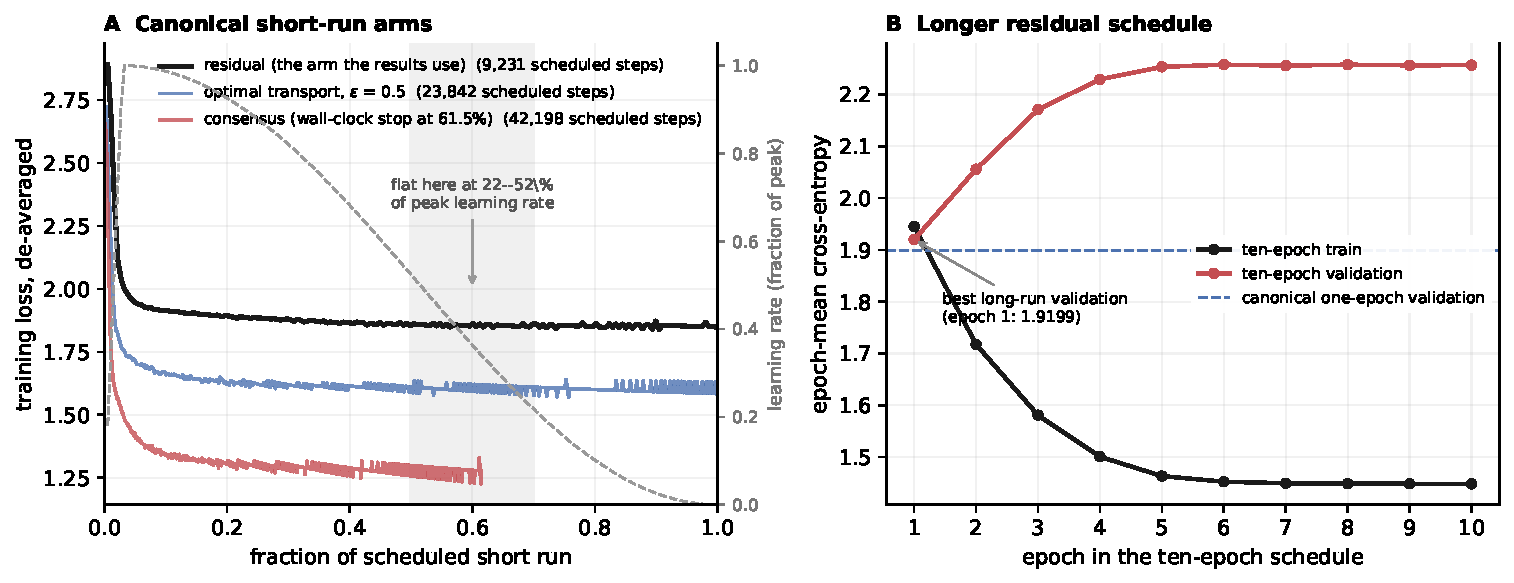
\includegraphics[width=\textwidth]{fig-training}
\caption[Training curves]{\textbf{The canonical short-run arms flatten, while a separate longer
residual schedule overfits on held-out cross-entropy.} \textbf{A}, de-averaged training loss against
fraction of the nominal one-epoch scheduler horizon for three target constructions. The residual
and optimal-transport arms complete their scheduled epoch; consensus was also scheduled for one
epoch but was terminated by the wall-clock at $61.5\%$. Three superseded residual builds are
omitted, as is the single-cell arm, whose training log was not retained. The dashed grey curve is
the canonical residual arm's learning rate relative to its post-warmup peak; the shaded band marks
$50$--$70\%$ of that horizon, where loss is already flat at $22$--$52\%$ of peak learning rate.
Absolute panel-A losses are not comparable between arms because their target strings differ.
\textbf{B}, epoch-mean losses for the separate ten-epoch residual schedule (nominal scheduler
horizon $92{,}318$; $92{,}310$ optimizer updates), with canonical one-epoch validation loss as a
dashed reference. No long-run checkpoint was scored with $\NIR$.}
\label{fig:training}
\end{figure}

\subsection{The identity test: failed designs and remaining guards}
\label{sec:app-identity}

The substitution test of Section~\ref{sec:res-mechanism} is the fourth design. The three that
failed are recorded here with their algebra, because each produced results this thesis previously
quoted as findings, and the constraints they teach are the surviving design.

\emph{Failed design one: mismatched geometry.} The first test overwrote drug A's code with drug
B's, inside a $\leq 10$-dimensional purified subspace, and compared the resulting KL against a
random vector of identical norm drawn in the \emph{full} $2048$-dimensional stream. Roughly
$99.5\%$ of the control's energy then lay in directions the intervention never touched, including
the cell-line directions measured at $\approx 0.6$ variance share. ``The swap moves the output less
than noise'' is exactly what that geometry predicts, whatever the readout does.

\emph{Failed design two: ablate-then-add.} The second drew the control inside the subspace, which
looked like a repair and was not. The hook ablates before adding, so what is delivered is (added
$-$ removed), and an uncentred class mean shares its global-mean component with the thing removed.
The substitution arm was then close to a restoration and the control arm a real displacement.
Simulated with no model present, the control delivers $5.3\times$ the perturbation in $100\%$ of
draws, with the predicted gap $2\langle \mu_B, u\rangle = 9.179$ against an observed $9.162$, where
$\mu_B$ is the injected class mean and $u$ the cell's own component in the slab. The retracted
result was geometry, not biology.

\emph{Failed design three: the normaliser.} The third injected the displacement and scored
$\Delta \log P(g_B)$ against a norm-matched random direction --- and was confounded the opposite
way. A random direction inside the slab does not follow the empirical class-mean geometry: it
inflates the logsumexp normaliser (measured $+2.75$ nats) where the observed class-mean displacement
does not, so every target is
depressed under the control arm whether or not it carries identity. With the scored target stripped
of all identity information, $36\%$ of the effect still stood. Norm-matched is not
disruption-matched. The same argument retires the simplest \emph{injection} test, ``how far did the
output move'': distance moved is exactly what norm-matching equalises, so that test has no power in
precisely the world where the readout does read the drug. It does not reach the behavioural
output-invariance instrument of Section~\ref{sec:methods-controls}, which perturbs the prompt rather
than the activations and matches no norms; that instrument's own limitation --- it registers whether
the output moves, not whether it moves correctly --- is stated where it is used.

Three further guards from the surviving design are engineering rather than inference and are
recorded here. A \emph{drug-proxy screen} refuses any context label that is a near-bijection with
drug --- it caught the metadata field \texttt{dose\_float} holding a sample identifier in the
residual builders, which, had it been orthogonalised against, would have deleted the drug axis by
construction. An \emph{injected-norm diagnostic} reports the displacement against the cell's
centred slab component ($0.69$--$1.40$: the injection is the size of the thing it displaces, so a
null cannot be blamed on a whisper). And a \emph{selftest with teeth} runs three planted worlds ---
drug inert, drug read, and drug inert behind a readout sensitive to displacement magnitude rather
than direction --- through the actual headline code path; it separates them ($-0.042$, $+1.520$,
$-0.010$), and it failed four times during development, each failure a real defect that the guard
list now covers. That third world is not a normaliser control: each planted response is a single
token, so nothing diverges, and the state-dependent part of the normaliser is precisely what the
selftest cannot exercise (Section~\ref{sec:res-mechanism}).

\subsection{Calibration self-test}
\label{sec:app-selftest}

The calibration framework of Section~\ref{sec:methods-metrics} is itself checked, since a metric
audit whose instrument is untested proves nothing. Beyond deterministic unit checks --- a perfect
prediction must reach the metric's maximum, a zero shift and a flat truth must return no score ---
the self-test asserts the exploit under a \emph{second, independent} zero-information baseline: a
leave-one-out mean scores $\DEdr = 1.000$ while $\NIR$ refuses to place it above chance. The
assertion in the code is exactly that --- $\NIR \leq 0.6$ --- and the value it records is $0.000$.
That $0.000$ is not the metric's chance value, which is $0.500$
(Section~\ref{sec:methods-metrics}) and is what the generic arm scores in
Tables~\ref{tab:lookup} and~\ref{tab:allarms}; nor is it the untied degeneracy that section
describes, since the self-test scores under the same half-tie convention as everything else here. It
is a property of this particular construction: the mean of the five other drugs resembles those five
more closely than it resembles the held-out one, so it loses every comparison. Two unrelated
constructions saturating the standard metric while neither is placed above chance by the
discrimination metric establishes the exploit as a property of the metric rather than of any one
baseline.

\end{document}
